\documentclass[12pt]{article}
\usepackage[a4paper, total={5.7in, 9in}]{geometry}
\usepackage{hyperref}
\usepackage{graphicx} % Required for inserting images
\usepackage{svg}
\usepackage{float}    % Required for the [H] specifier
\usepackage{listings}
\usepackage{xcolor} % Required for custom colors
\usepackage{subcaption}
\usepackage{lmodern}
\usepackage[T1]{fontenc}
\usepackage{multirow}

% Define custom colors for code
\definecolor{codegray}{rgb}{0.5,0.5,0.5}
\definecolor{backcolour}{rgb}{0.95,0.95,0.92}

\lstset{
    backgroundcolor=\color{backcolour},   
    basicstyle=\ttfamily\small, % This makes it look like code (monospaced)
    keywordstyle=\bfseries,
    numberstyle=\tiny\color{codegray},
    stringstyle=\color{codegray},
    breakatwhitespace=false,         
    breaklines=true,                 
    captionpos=b,                    
    keepspaces=true,                 
    numbers=left,                    
    numbersep=5pt,                  
    showspaces=false,                
    showstringspaces=false,
    showtabs=false,                  
    tabsize=2
}

\begin{document}
\title{No Friends, No Problem: Can AI Play Werewolf?}
\author{Ninivaggi Luca s5312342\\
{\em ninivaggiluca@gmail.com}}
\date{}
\maketitle        

\section{Details of the Proposal}
\label{sec:yourProposal}

The proposed project is a Jason-based implementation of the social deduction game ``Werewolf''\footnote{The implemented game follows a slightly modified version (thoroughly explained in subsection ~\ref{subsec:modifiedRules}) of the traditional rules, that can be found at \cite{mafia_wiki}.}.

The project is developed using the MAS infrastructure provided by \emph{Jason}, utilizing a headless adaptation of the \emph{VEsNA-Pro} engine renamed \emph{Jason-Pro}. The game relies entirely on explicit message exchange and internal  logical states, hence the physical environment managed (by design) with\emph{VEsNA} was removed altogether. 

The actual reasoning cycle driving each player's decisions is exclusively handled by a Large Language Model (LLM), a purely symbolic engine, or a real human interacting via a User Interface (UI). 

Within this architecture, all game logic, behavior definition  and state management are strictly handled by the \textbf{Jason Engine}, with the \textbf{LLM} used as a "Natural Language Generator" and the \textbf{UI} as a visualization tool of the player's state.

Within this context, was also conducted a fine-tuning on a instance of BERT\cite{devlin-etal-2019-bert} to try to implement a non-LLM recognition of the speech-act carried by the players, in order to deal with the \emph{Linguistic  Relativism} inherently present in any not-standardized communication exchange.

\subsection{Full Specification of Your Proposal}
\label{subsec:specification}

The primary goal of this project is to deliver a fully functional, real-time playable game where autonomous agents behave according to their dynamic internal states. 

In this context, the pursuit of  flawlessly strategic gameplay is not the goal: the core objective is to ensure that the agents interact in an \emph{organic} manner, making unpredictable but coherent decisions that genuinely reflect their fluctuating psychological moods and relational variables. 

To achieve this organic social deduction environment, the system's architecture is practically realized through three modules:

\paragraph{Game Engine (S\&DAI):}
This module functions as the standalone kernel of the Jason MAS. 

Fundamentally, the system is defined by exactly one Narrator and $K$ players communicating exclusively through native Jason performatives. These messages carry strict logical semantics for the engine but entirely lack human-readable natural language (e.g., message are exchanged as  \texttt{speech(accuse(Alice), "")}). 

The Narrator dictates the flow of the game by strictly following an internal game graph, managing phase transitions, synchronization, and rule enforcement. 
In contrast, the players act as abstract, reactive objects that require an attached reasoning engine to operate: in this baseline implementation, decision-making is handled by the built-in symbolic reasoner, which is driven by \emph{Jason-Pro} parsing logic. 


\paragraph{Role-Play simulated experience (NLP):}
To transform the dry exchange of logical predicates into an immersive social deduction experience, a custom Java bridge queries a local instance of Ollama. Within this architecture, the Large Language Model can serve two distinct functions:
\begin{itemize}
    \item \textbf{As a Natural Language Generator (NLG):} It translates the Narrator's structural phase transitions and the agents' chosen symbolic performatives (e.g., \texttt{accuse(alice)}) into coherent, role-played dialogue. 
    To maintain logical consistency, this text generation is heavily constrained by prompts derived directly from the agent's current state (such as their specific personality traits and momentary moods, or the epistemic beliefs about other players), ensuring the output never contradicts their symbolic intentions.
    
    \item \textbf{As a Sub-Symbolic Reasoner:} By utilizing the Jason agent as a structural wrapper, the LLM automatically manages the agent's dynamic internal state. It uses the current symbolic variables (personality and moods) alongside recent game logs as context to evaluate the social environment. 
    It can also manage its internal state and beliefs about other players to directly drive the agent's future logical actions and plan selections, seamlessly bridging complex social analysis with BDI execution.
\end{itemize}

Furthermore, an attempt was made to deal with the \emph{Linguistic  Relativism} inherently present in any not-standardized communication exchange. For academic purposes, is proposed a non-LLM implementation of the recognition of the speech-act carried by the  players. Incremental solution were proposed, each one improving the previous one, each one tackling the problem using a pre-trained BERT in slightly different ways. The results (and limitations) of this approach are thoroughly discussed in the dedicated section.

\paragraph{User Interface (UI):}
The UI serves a dual purpose. For the AI agents, it acts as a real-time observation tool, visualizing their shifting moods, epistemic beliefs, and target choices through an explicit visualization. 
For a human player, it provides a structured interface that strictly guides their input. By forcing the human to select valid performatives and targets via GUI buttons while allowing free-text message generation, the system ensures that human actions perfectly align with the MAS network and do not break the underlying Prolog logic.

\subsection{Type of project}
\label{subsec:kind}
Joined creative project NLP + S\&DAI


\subsection{Difficulty Range}
\label{subsec:points}
\textbf{HARD} - max 15.5 Points

\tableofcontents

 \section{Introduction}
\label{sec:intro}
% Introduce the concept of Social Deduction Games and why playing them with BDI agents and LLMs is an interesting challenge. Outline the structure of the report.
\subsection{Modified Set of Rules}
\label{subsec:modifiedRules}

While the original rules of the game are documented in \cite{mafia_wiki}, several structural modifications were implemented in this project. 
These changes are designed to enhance the realism of the game, accommodate the erratic behavior of the agents, and improve the user experience for human players:

\begin{itemize}
    \item \textbf{Flexible Role Assignment:} The traditional recommendation of a 1:3 ratio between Werewolves and Villagers is not strictly enforced; the game can be initialized with any arbitrary numerical distribution of roles by simply defining a custom set of players and roles within the \texttt{werewolf.jcm} file.
    
    \item \textbf{Nocturnal Hunt Mechanics:} During the night phase, Wolves select a victim using a \emph{plurality vote} (the highest vote count wins). To simulate realistic behavior (e.g. players that does not really understand the goal of the game), Wolves are allowed to vote for other Wolves. Since text communication is disabled at night, they are granted up to \textbf{3 consecutive voting rounds}\footnote{This allows the wolves to to silently coordinate by observing each other's previous votes; else they have no way to align themselves, since the only phase with explicit communication is the public Discussion Phase.}. If a tie remains after the third round, the hunt fails and no player is eliminated.
    
    \item \textbf{Structured Discussion Phase:} The daytime discussion is strictly limited to an exchange of exactly  \textbf{7 messages}. The floor is granted to players who explicitly request to speak, resolved through a strict priority hierarchy (Subsection \ref{subsubsec:speaker_selection}).

    
    \item \textbf{Daytime Execution Vote:} The village execution vote consists of a single voting round utilizing the same plurality system as the nocturnal hunt. In the event of a tie, no execution takes place and the game proceeds to the next night phase.
    
    \item \textbf{Terminal Conditions:} The game only concludes upon the total annihilation of one faction: either all Wolves are eliminated, or all Villagers are eliminated. This intentionally deviates from the standard rule where Wolves win automatically upon reaching numerical parity with the Villagers\footnote{This change allows for edge cases where a dominant Wolf pack might still lose the game due to erratic internal voting or self-sabotage.}.
\end{itemize}

\subsection{Overview of the Project}
\label{subsec:overview}

The in-depth explanation of the project's functionalities follows a layered approach, starting from the most bare-bones version of the system, consisting solely of the core game engine driven by the \textbf{Narrator} (Section \ref{sec:narrator}) and the purely symbolic \textbf{players} (Section \ref{sec:players}). 

\begin{figure}[H]
    \centering
    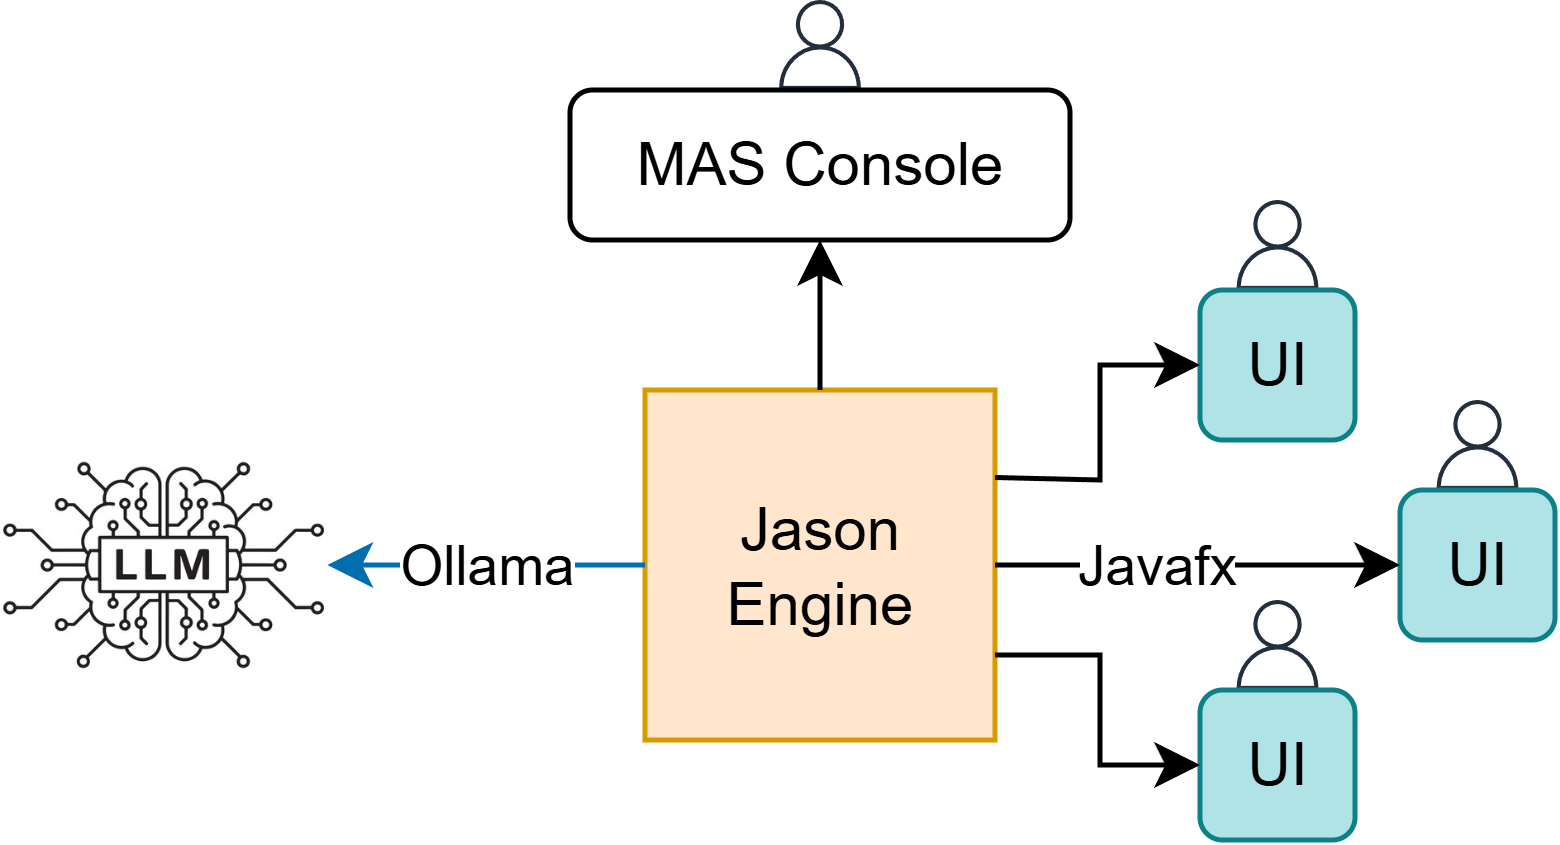
\includegraphics[width=0.8\textwidth]{images/schema.png}
    \caption{High-level schematic of the project modules: the Jason engine acts as the bare-bone central orchestrator, Ollama provides LLM capabilities, and JavaFX drives the User Interfaces.}
    \label{fig:architecture_schema}
\end{figure}

Building upon this standalone symbolic core, we subsequently introduce the \textbf{JavaFX User Interface} (Section \ref{sec:ui}) to enable human-driven player interactions and spectator observability. Finally, we detail the custom \textbf{Ollama API} (Section \ref{sec:llm}), which is integrated into the architecture to facilitate both Natural Language Generation (NLG) and reasoning for LLM-driven autonomous players.


\section{The Narrator Agent}
\label{sec:narrator}

The Narrator serves as the sole truth-keeper in the game: it holds beliefs about the current state of the game, along with the complete \emph{log} (see Subsection \ref{subsec:logging}), which can be used as context by other agents when needed. It orchestrates all game interactions by simulating a \textbf{graph traversal} on its internal state machine.

\subsection{Setup and Settings Configuration}
\label{subsec:narrator-setup}

At the start of the MAS simulation, the Narrator is the only agent that "wakes up". Its first task is to define the simulation's settings, along with verifying everything is coherent such as "pinging" the \emph{Ollama bridge} (Section \ref{sec:llm}) to verify that it is correctly set up and available.

The code regarding this part is defined in the file \texttt{narrator/init\_narrator.asl}, where the baseline configuration is defined by a hard-coded schema containing default values and scope annotations (either \texttt{[local]} for Narrator-exclusive settings or \texttt{[share]} for settings that must be broadcast to all players, such as the inability to utilize the LLM if the ping fails). 

However, those parameters can be easily tinkered by the user, directly by editing the \texttt{werewolf.jcm} file without modifying the underlying agent's code (Listing \ref{lst:jcm_setup} propose a example of a custom configuration).

During the \texttt{setup} execution, the Narrator parses these overriding beliefs. Any setting provided in the \texttt{werewolf.jcm} file that does not exist in the predefined whitelist is immediately rejected and abolished to prevent logical errors; the accepted settings are then updated. 

\vspace{1em}
\begin{lstlisting}[frame=single, language=Prolog, caption={Example configuration in the \texttt{werewolf.jcm} file overriding the default Narrator settings: is defined a  specific LLM model, the maximum number of rounds to hunt or speak is changed and all the \emph{artificial} delays are removed.}, label={lst:jcm_setup}]
agent narrator : narrator.asl {
    beliefs:  setting(llm_model("gemma4:31b")),
              setting(max_hunt_rounds(5)),
              setting(max_discussion_turns(10)),
              setting(disable_delay(true))
}
\end{lstlisting}

Once the Narrator's configuration is fully set up, it broadcasts the \texttt{[share]} settings to all active players and waits for them to acknowledge their configurations before officially starting the game.


\subsection{The Game Graph}
\label{subsec:game-graph}

The flow of a Werewolf game is inherently cyclical and phase-based (e.g., Night falls, Wolves hunt, Day breaks, Village discusses, Village votes). To formally define the execution of the state machine, the Narrator relies on a directed multi-edge graph engine defined within the \texttt{game\_graph.asl} file. 

\begin{figure}[H]
    \centering
    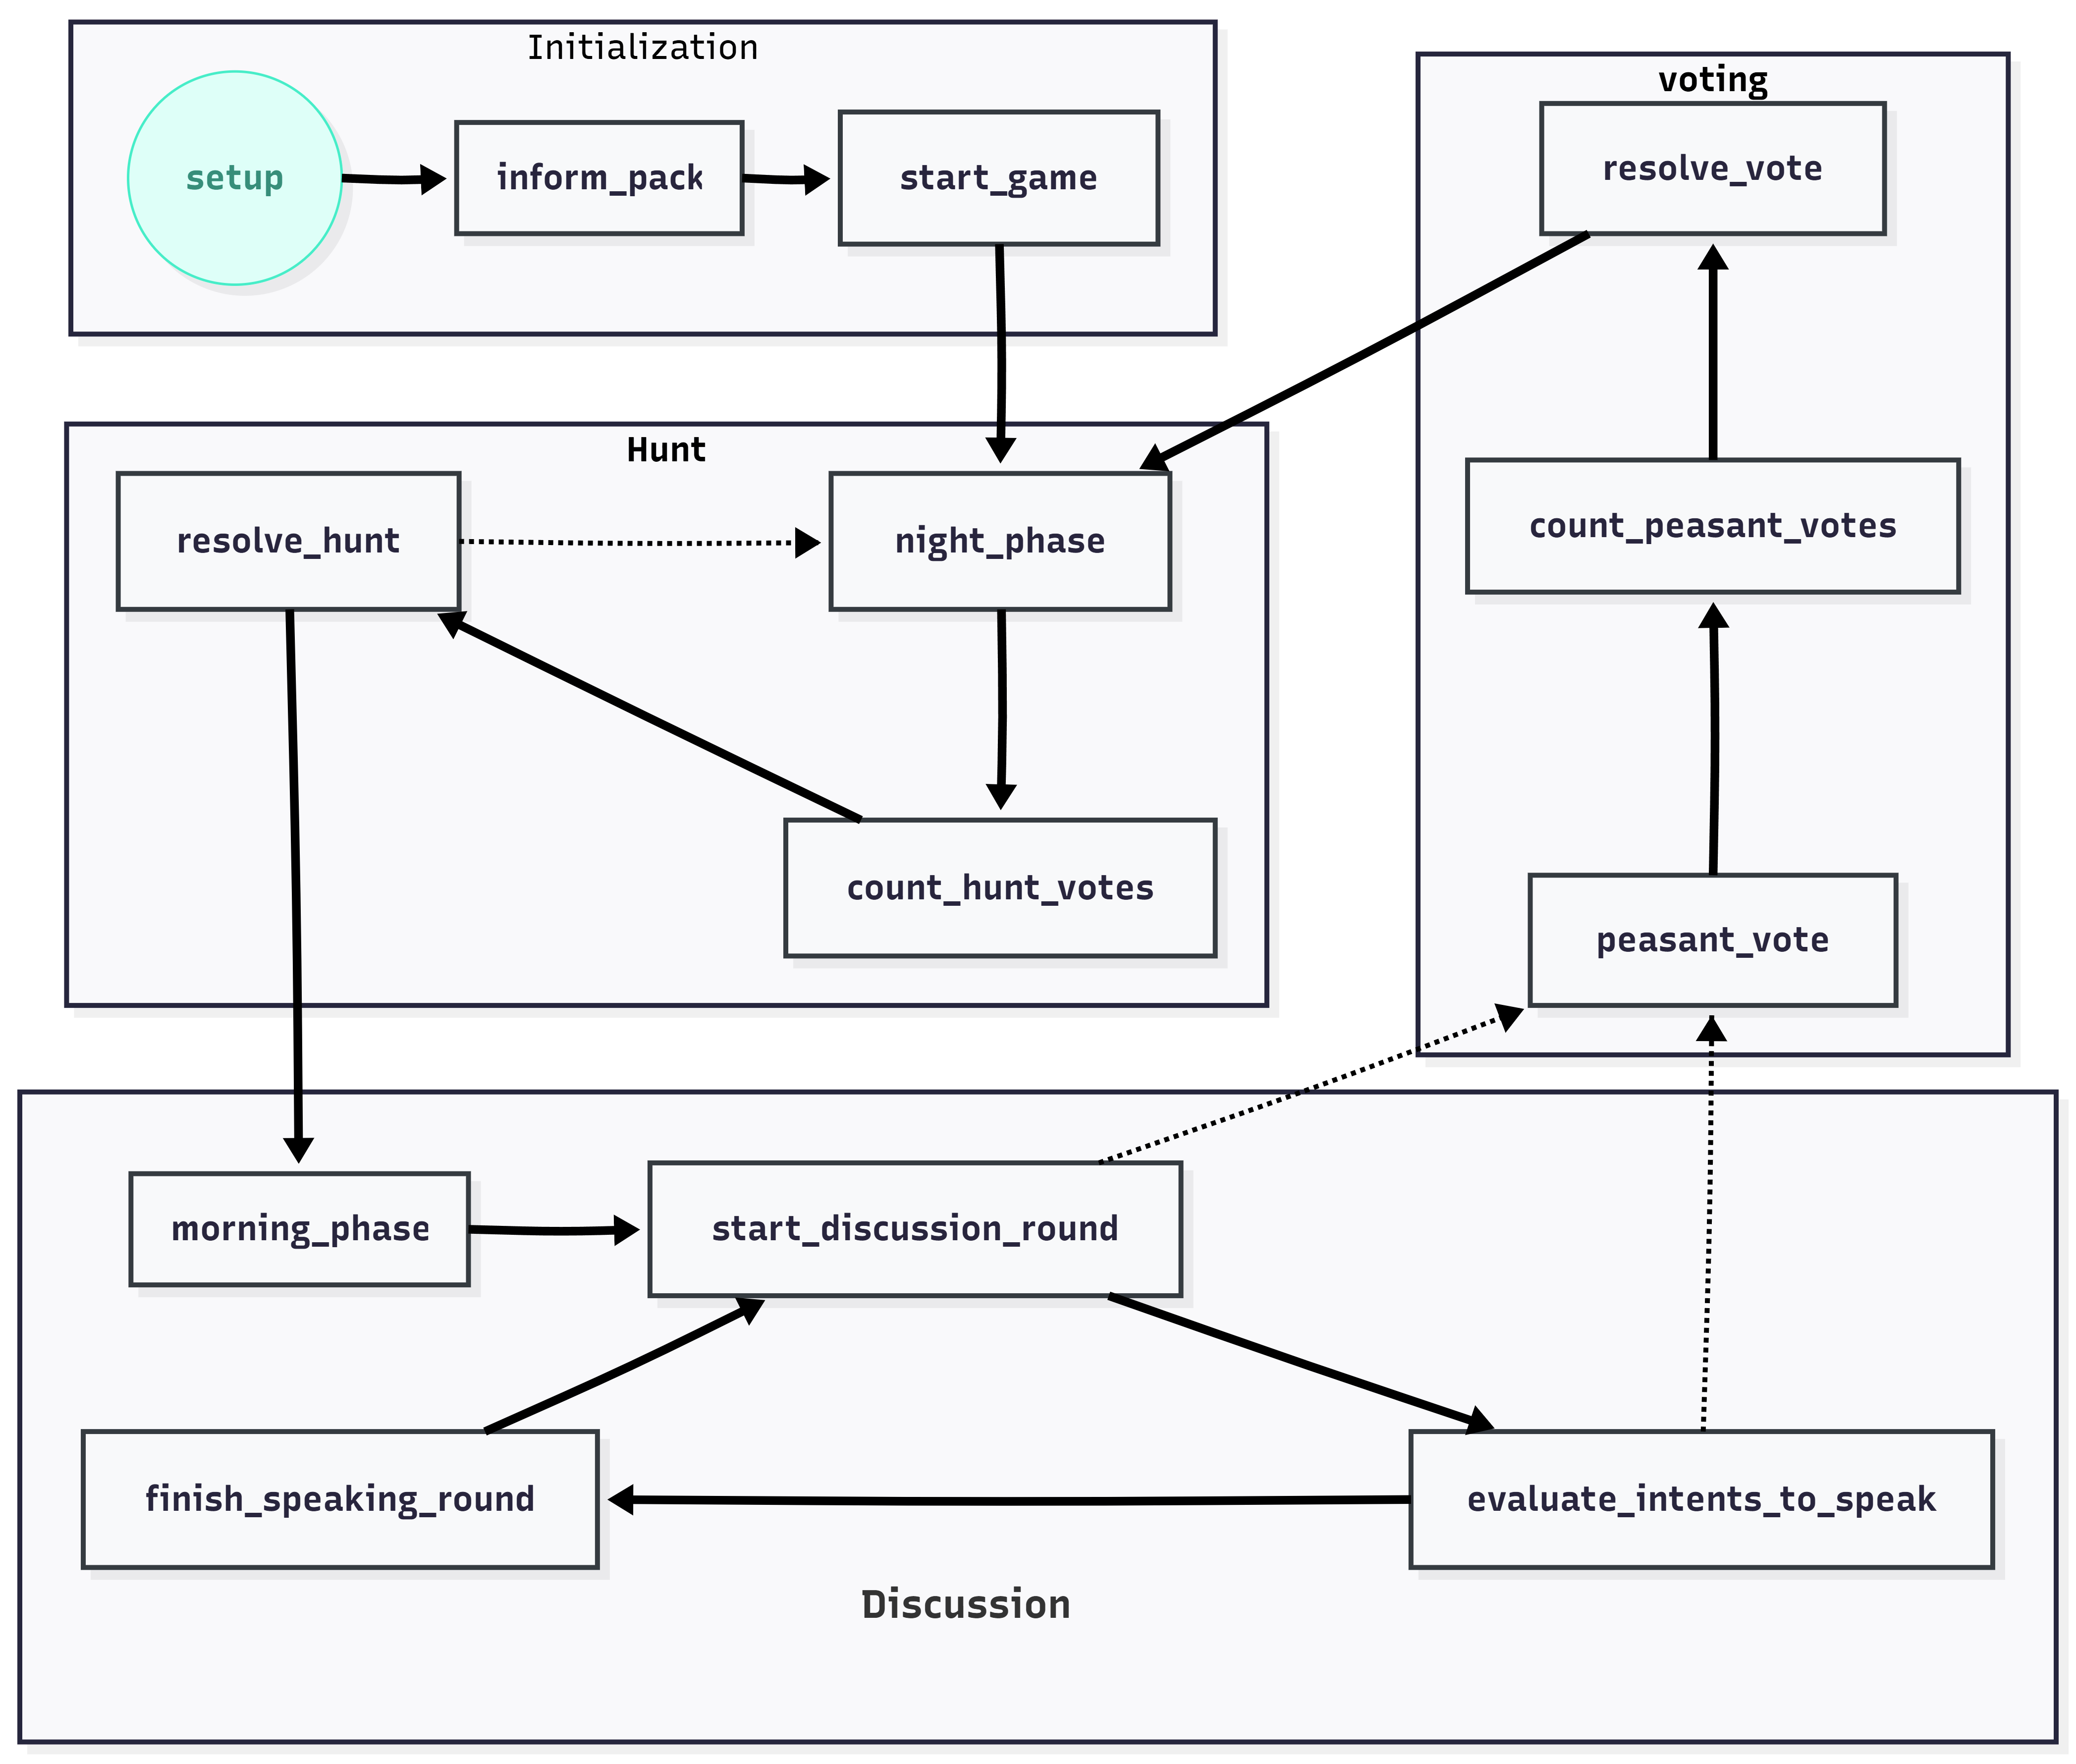
\includegraphics[width=\textwidth]{images/full_game_graph.png}
    \caption{Symplified visualization of the state machine representing the game phases and transitions.}
    \label{fig:master_graph}
\end{figure}

The graph is formalized using rule-based beliefs natively implemented in Jason, allowing the engine to represent complex game states and conditional branching within a  ``user-readable`` implementation. 

\subsubsection{Nodes}
Every state in the game is represented as a node structured as a triplet $$\texttt{node(EnterAction, NodeName, CleanUpList)}$$ 

The \texttt{EnterAction}, if defined, is an \texttt{action(Audience, ActionName)} that is broadcast to all players within the \texttt{Audience} (a subset of the alive players), who must then respond to, to release a \texttt{sync\_barrier} set up to synchronize them (see Subsection \ref{subsec:sync-barrier}).

On the other hand, \texttt{CleanUpList} is a list of beliefs that are abolished once the Narrator leaves the node (since they fulfill their purpose). This prevents the belief base from becoming cluttered and mitigates the risk of invalid states.

\vspace{1em}
\begin{lstlisting}[frame=single, language=Prolog, caption={Example of a node definition representing the Daytime Voting Phase: to every player is injected the goal \texttt{choose\_vote}, and from the narrator itself is abolishe the  belief about the last person who spoke.}, label={lst:peasant_vote_node}]
node(
    action(TargetList, choose_vote), 
    peasant_vote, 
    [last_speaker(_)]
) :- players(TargetList).
\end{lstlisting}

\subsubsection{Edges}

The transitions are modeled as a multi-edge graph, meaning multiple distinct paths can exist between the same two nodes depending on the game's context (e.g., a tied vote versus a decisive execution). An edge is defined as $$\texttt{edge(FromNode, Message, ToNode)}$$ 

Each \texttt{Message} is further defined as a complex structure \footnote{Each on of those ``structures`` are actually Jason's beliefs, each time verified on-the-fly to ensure a graph traversal coherent witht the current game's state.} defined as $$\texttt{msg(Players, PhaseMsg, PhaseTitle, Action)}$$ which describes exactly what is broadcast to all players (or a subset of them) during the transition:
\begin{itemize}
    \item \textbf{\texttt{Players}:} The target audience receiving the transition message.
    \item \textbf{\texttt{PhaseMsg} \& \texttt{PhaseTitle}:} Narrative text elements, mainly used to update the LLM context or the UI.
    \item \textbf{\texttt{Action}:} is the actual \emph{speech-act} of the message, i.e. the actual logic information that the players use to  update their belief base.
\end{itemize}

\begin{figure}[H]
    \centering
    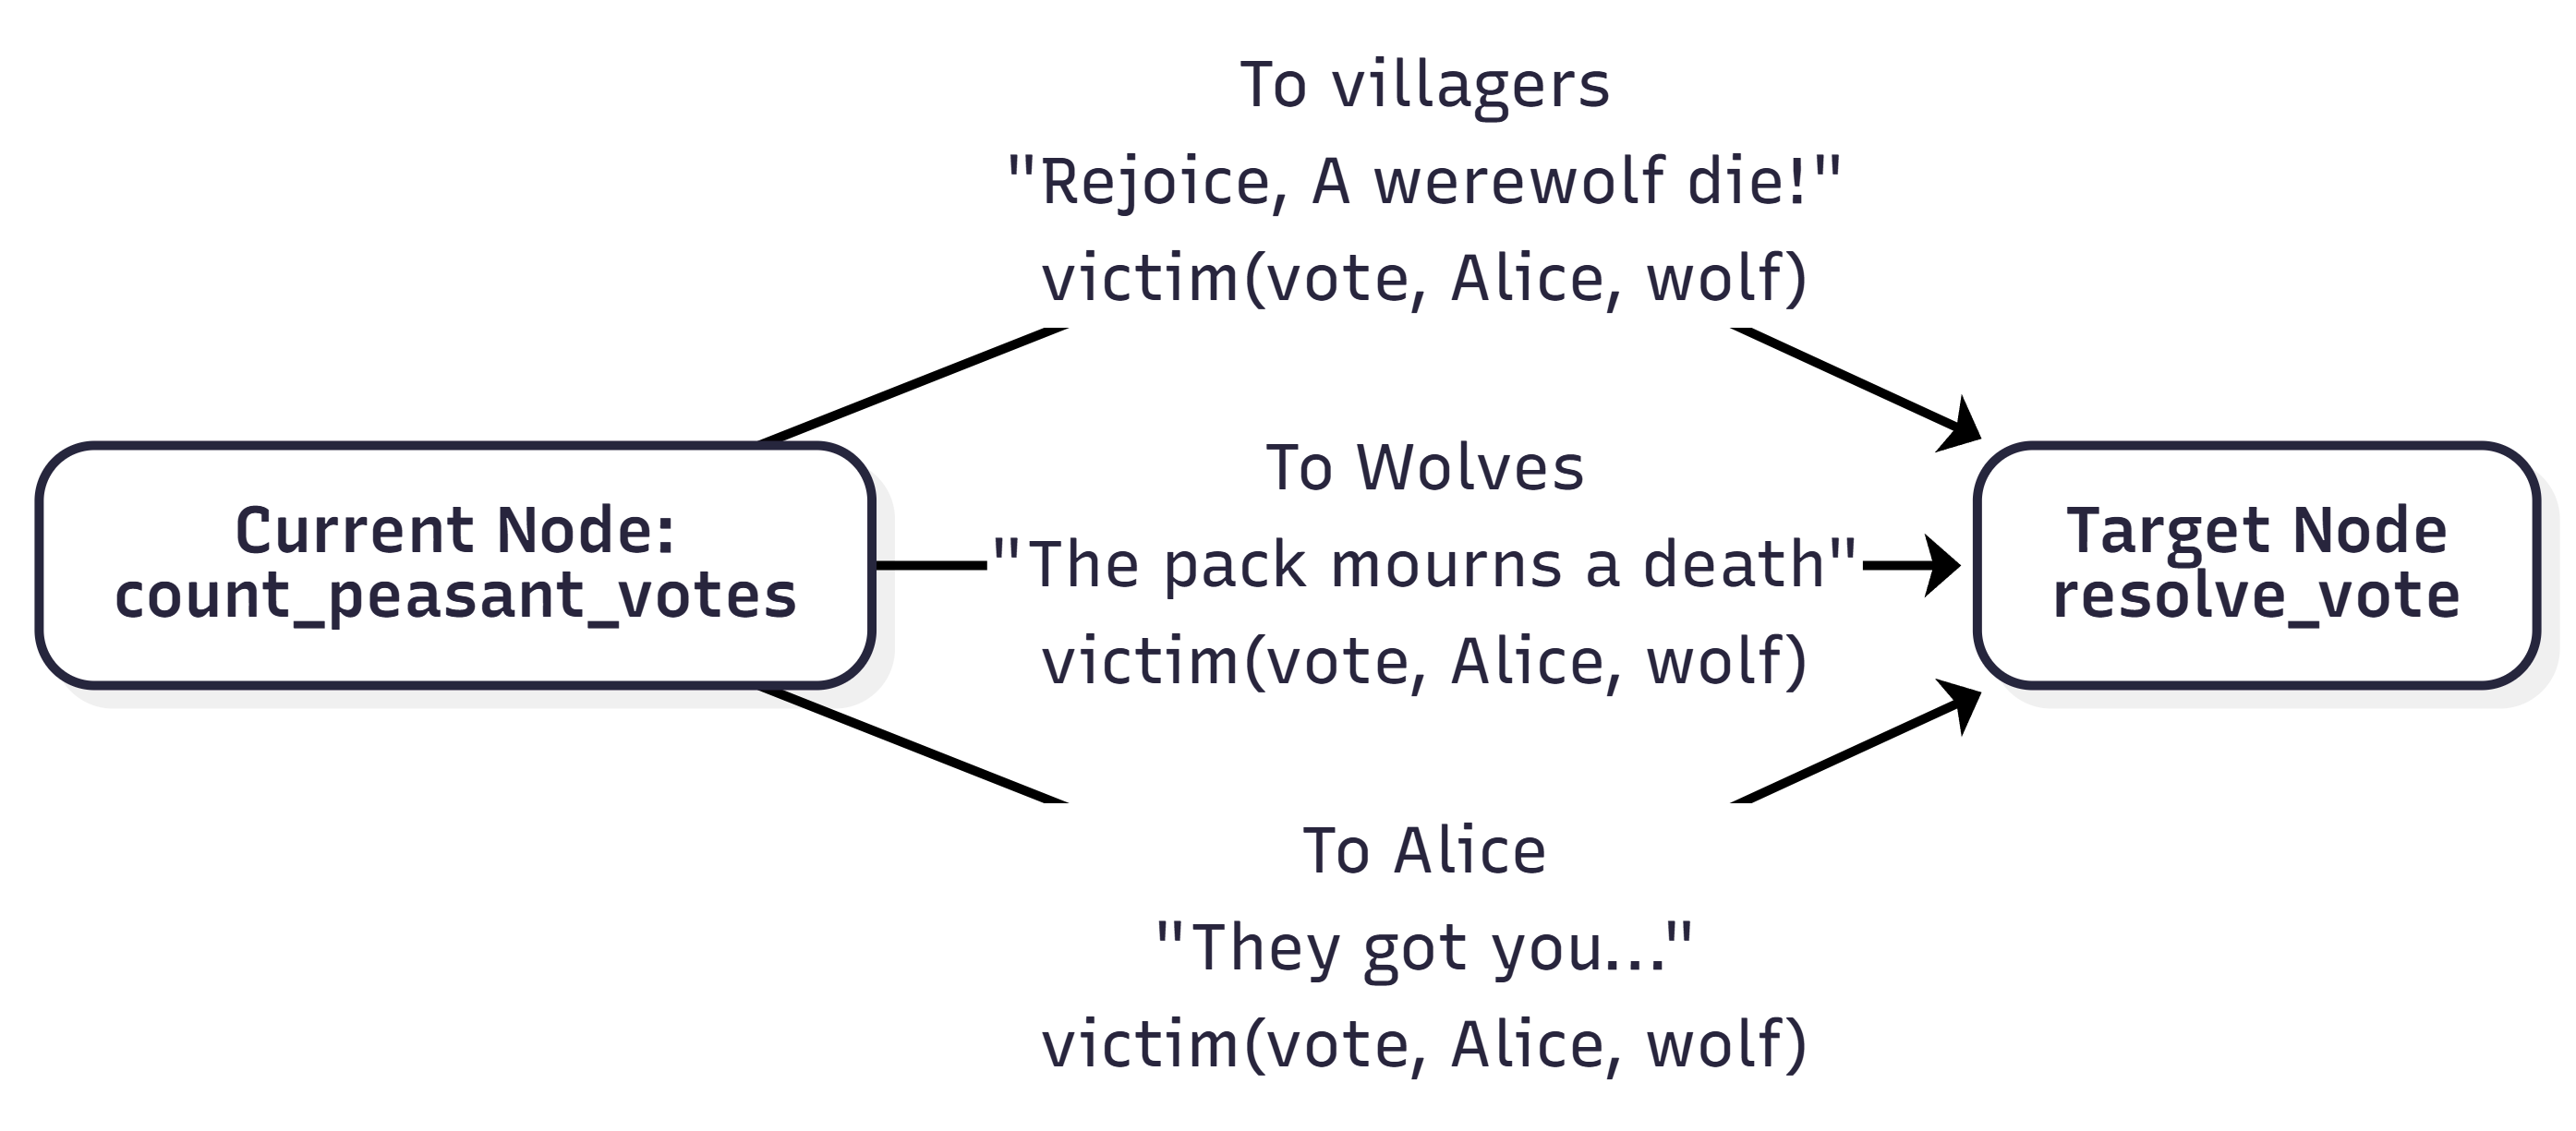
\includegraphics[width=\textwidth]{images/edge example.png}
    \caption{Example of a edge with multiple instances that can be activated at the same time, used to communicate that the Daytime Voting Phase has ended with a victim; different messages are sent to different audiences.}
    \label{fig:edge example}
\end{figure}


\subsubsection{Executing the Transition}
The core phase progression is handled by the Narrator's \texttt{execute\_transition} plan, as illustrated in Figure \ref{fig:transition_sequence}.

The plan executes all the subroutines needed to change the belief base, to bridge between phases.
When a phase concludes, the transition is executed:

\begin{enumerate}
    \item \textbf{Edge Evaluation and Exit:} The Narrator evaluates the current beliefs to select a valid outgoing \texttt{edge}. It then triggers the \texttt{ExitAction} of the current node to clean up the outgoing state.
    
    \item \textbf{Broadcast and Dispatch:} The Narrator extracts all valid \texttt{msg} payloads associated with the evaluated transition. It iterates through this collection and dispatches each payload to the specified \texttt{Players}\footnote{The players' reactions to these goals injected into their goal base are thoroughly explained in Section~\ref{sec:players}.}.
    
    \item \textbf{Node Entry and Synchronization:} The Narrator evaluates the new node's entry definition. If an explicit \texttt{EnterAction} is defined, the Narrator dispatches this action to the specified \texttt{Players} (e.g., instructing them to cast a vote) and immediately erects a \textbf{Synchronization Barrier} (detailed in Section \ref{subsec:sync-barrier}). The Narrator halts its internal game loop, waiting until it receives the corresponding \texttt{sync\_reply} responses from all targeted agents before proceeding. If no entry action is defined, the Narrator bypasses the barrier and directly executes the node's internal logic.
\end{enumerate}

\begin{lstlisting}[frame=single, language=Prolog, caption={Simplified Jason logic for the Narrator's transition engine (UI/LLM logics are removed for sempliticy).}, label={lst:transition_engine_code}]
+!execute_transition 
    : current_node(CurrentNode) 
    & edge(CurrentNode, _, NextNode)
    <-  !process_transition(CurrentNode, NextNode).

+!process_transition(CurrentNode, NextNode)
    <-  .findall(OutgoingMsg, 
            edge(CurrentNode, OutgoingMsg, NextNode), 
            AllMessages);
        
        ?node(_, CurrentNode, CleanupList);
        for ( .member(StaleBelief, CleanupList) ) 
        { .abolish(StaleBelief); };
        
        !activate_node(NextNode, AllMessages).

+!activate_node(NodeName, AllMessages)
    <-  -+current_node(NodeName);        
        for ( .member(OUT, AllMessages) ) {
            if (OUT = msg(TargetList,
                    BaseMessage, PhaseTitle, PhaseIntent, 
                    Actions_to_log)
                ) {
                
                !dispatch_phase(
                    TargetList, NodeName, 
                    PhaseTitle, BaseMessage);
                    
                for ( .member(Action, Actions_to_log) ) 
                { !dispatch_action(TargetList, Action); };
                
            };
        };

        ?node(IN, NodeName, _);
        if (IN = action(ActionTargets, Action)) {
            -+waiting_on(ActionTargets);
            .send(ActionTargets, achieve, Action);
        } else {
            !NodeName;
        }.
\end{lstlisting}

\begin{figure}[H]
    \centering
    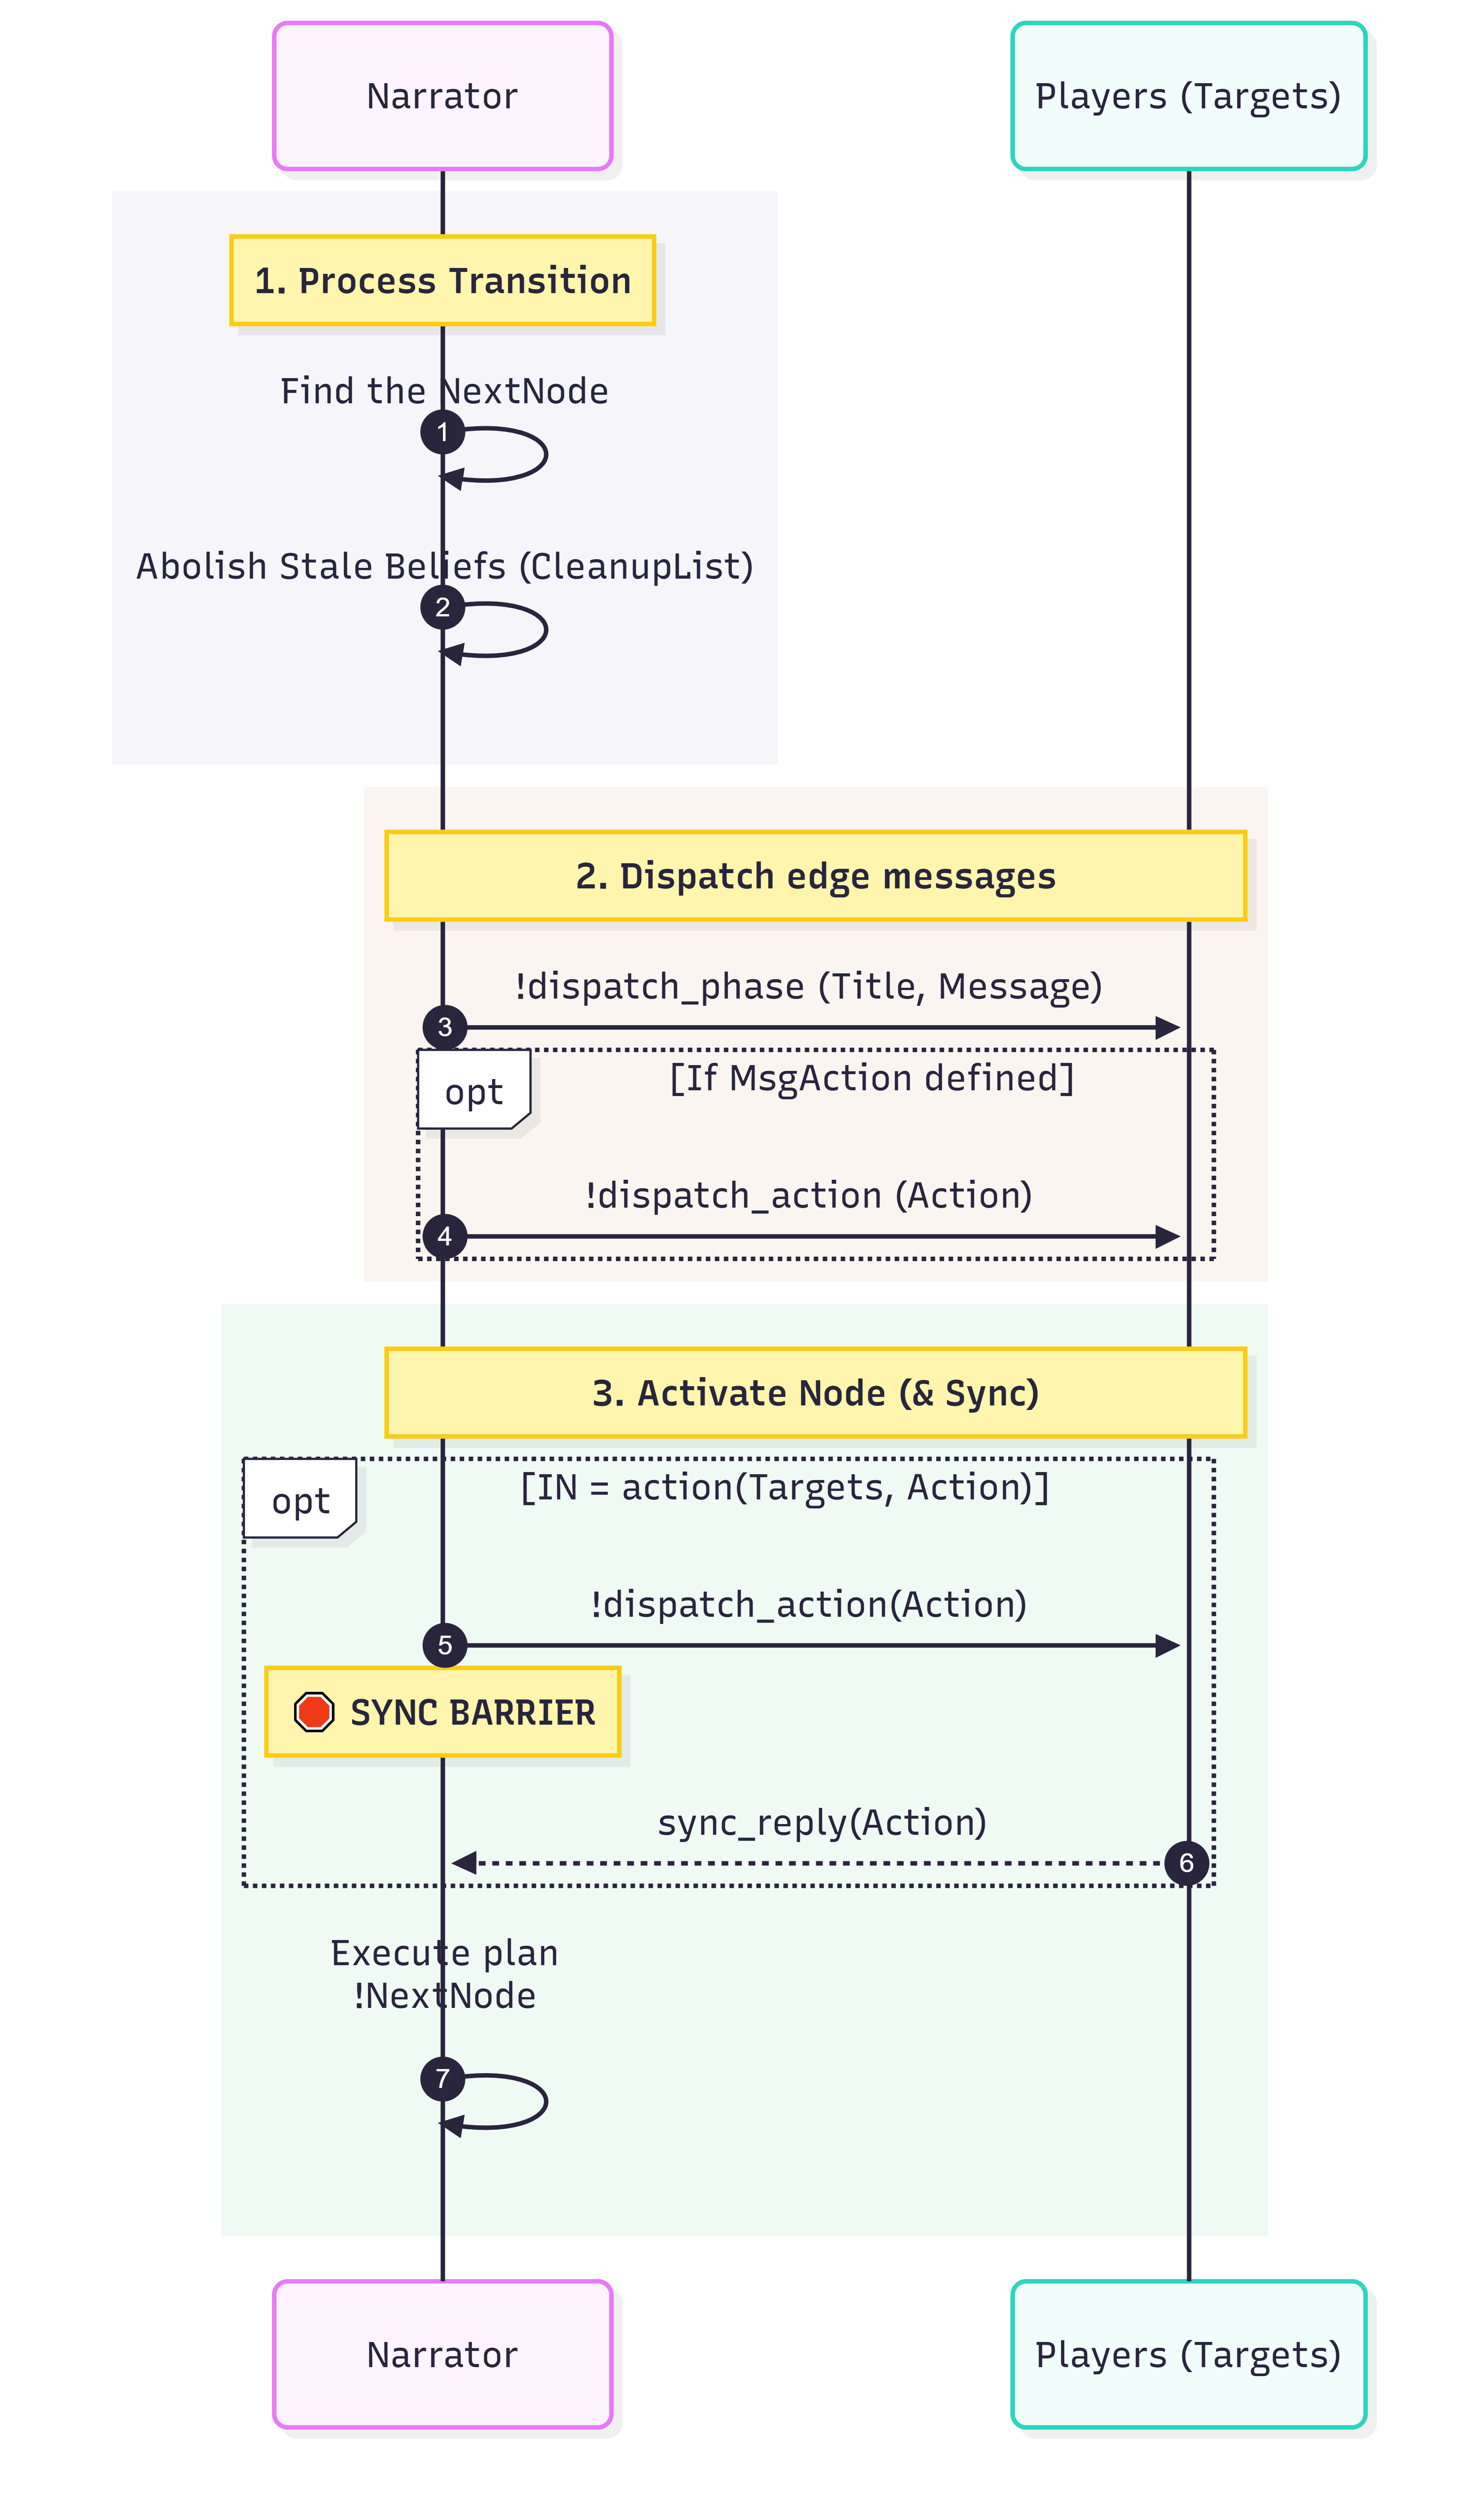
\includegraphics[width=\textwidth, height=0.95\textheight, keepaspectratio]{images/transition_phase_diagram.png}
    \caption{Sequence diagram illustrating the \texttt{execute\_transition} logic: the narrator can be halted in until some specific player responds to it, to synchronize their state.}
    \label{fig:transition_sequence}
\end{figure}



\subsection{Synchronization Barrier}
\label{subsec:sync-barrier}

Because the game relies entirely on message exchange and logical states, preventing race conditions and desynchronization between agents is critical\footnote{In this context, utilizing an engine explicitly optimized for proactivity, such as Jason, is arguably a disadvantage. It needs the implementation of slow, custom-built synchronization barriers that \emph{de facto} nullify the agents' proactive capabilities.}. If agents were allowed to send actions to the Narrator or to each other at any arbitrary time, the Multi-Agent System would quickly fall into an invalid state (e.g., an agent attempting to cast a vote while another is still finishing a speech). 

Furthermore, unregulated message broadcasting would result in agents observing and reacting to game events in different chronological orders: this temporal misalignment would inevitably corrupt their reasoning processes and destroy their ability to strategically align with one another.

To solve this, the architecture strictly enforces a unidirectional flow of control: \textbf{players are entirely reactive}. The \emph{only} way for a player to communicate an action back to the Narrator is by replying to a specific prompt using the \texttt{sync\_reply(Payload)} performative. 

\subsubsection{Technical implementation}
When the Narrator enters a node that requires player interaction (e.g., an \texttt{EnterAction} like \texttt{action(Targets, choose\_vote)}), it generates a \texttt{waiting\_on(Targets)} belief containing a list of all authorized agents. The internal graph traversal halts, and the Narrator becomes a passive listener waiting for \texttt{sync\_reply} messages.

\vspace{1em}
\begin{lstlisting}[frame=single, language=Prolog, caption={The Synchronization and Payload Management mechanics from the narrator; it is passively waiting for external messages from the players.}, label={lst:sync_logic}]
@sync_handler[atomic]
+!sync_reply(Payload)[source(Sender)]
    : waiting_on(WL) & .member(Sender, WL) 
    <-  +Payload;
        !manage_sync_payload(Payload);
        .delete(Sender, WL, NewWL);
        if (NewWL == []) {
          -waiting_on(_);
          !execute_transition;
        } else {
          -+waiting_on(NewWL);
        }.

//Example: votes are managed by mirroring them to all agents
+!manage_sync_payload(vote(Voter, Target)) 
    : players(AllPlayers)
    <-  !dispatch_action(AllPlayers, vote(Voter, Target)).
\end{lstlisting}

The resolution of this barrier operates in three distinct steps, as defined in the Jason logic (Listing \ref{lst:sync_logic}):

\begin{enumerate}
    \item \textbf{Sender validation:} When a \texttt{sync\_reply} arrives, the Narrator first verifies that the sender is currently in the \texttt{waiting\_on} list. If valid, the payload is accepted and the sender is removed from the list (if a player response, even if it is not on the waiting  list, something is irremediably wrong).
    
    \item \textbf{Payload Management \& Dispatch:} The narrator then processes the received payload (e.g., a vote or a speech from a player) via \texttt{manage\_sync\_payload}\footnote{Is overloaded in the plan base, and at runtime is called the suitable one; unexpected payloads are correctly notified.}. The Narrator explicitly dispatches this payload as an \texttt{action} to all relevant players in the game. This ensures that every player manages the event in the same order, maintaining the Narrator as the absolute single source of truth and avoiding P2P communications.
    
    \item \textbf{Barrier Release:} Once the \texttt{waiting\_on} list becomes completely empty, the Narrator destroys the barrier belief and safely resumes the graph traversal by calling \texttt{!execute\_transition} to proceed to the next node.
\end{enumerate}


Figure \ref{fig:sync_sequence} visualizes this exact flow, demonstrating how the Narrator processes concurrent replies while maintaining global synchronization through intermediate dispatching.

\begin{figure}[H]
    \centering
    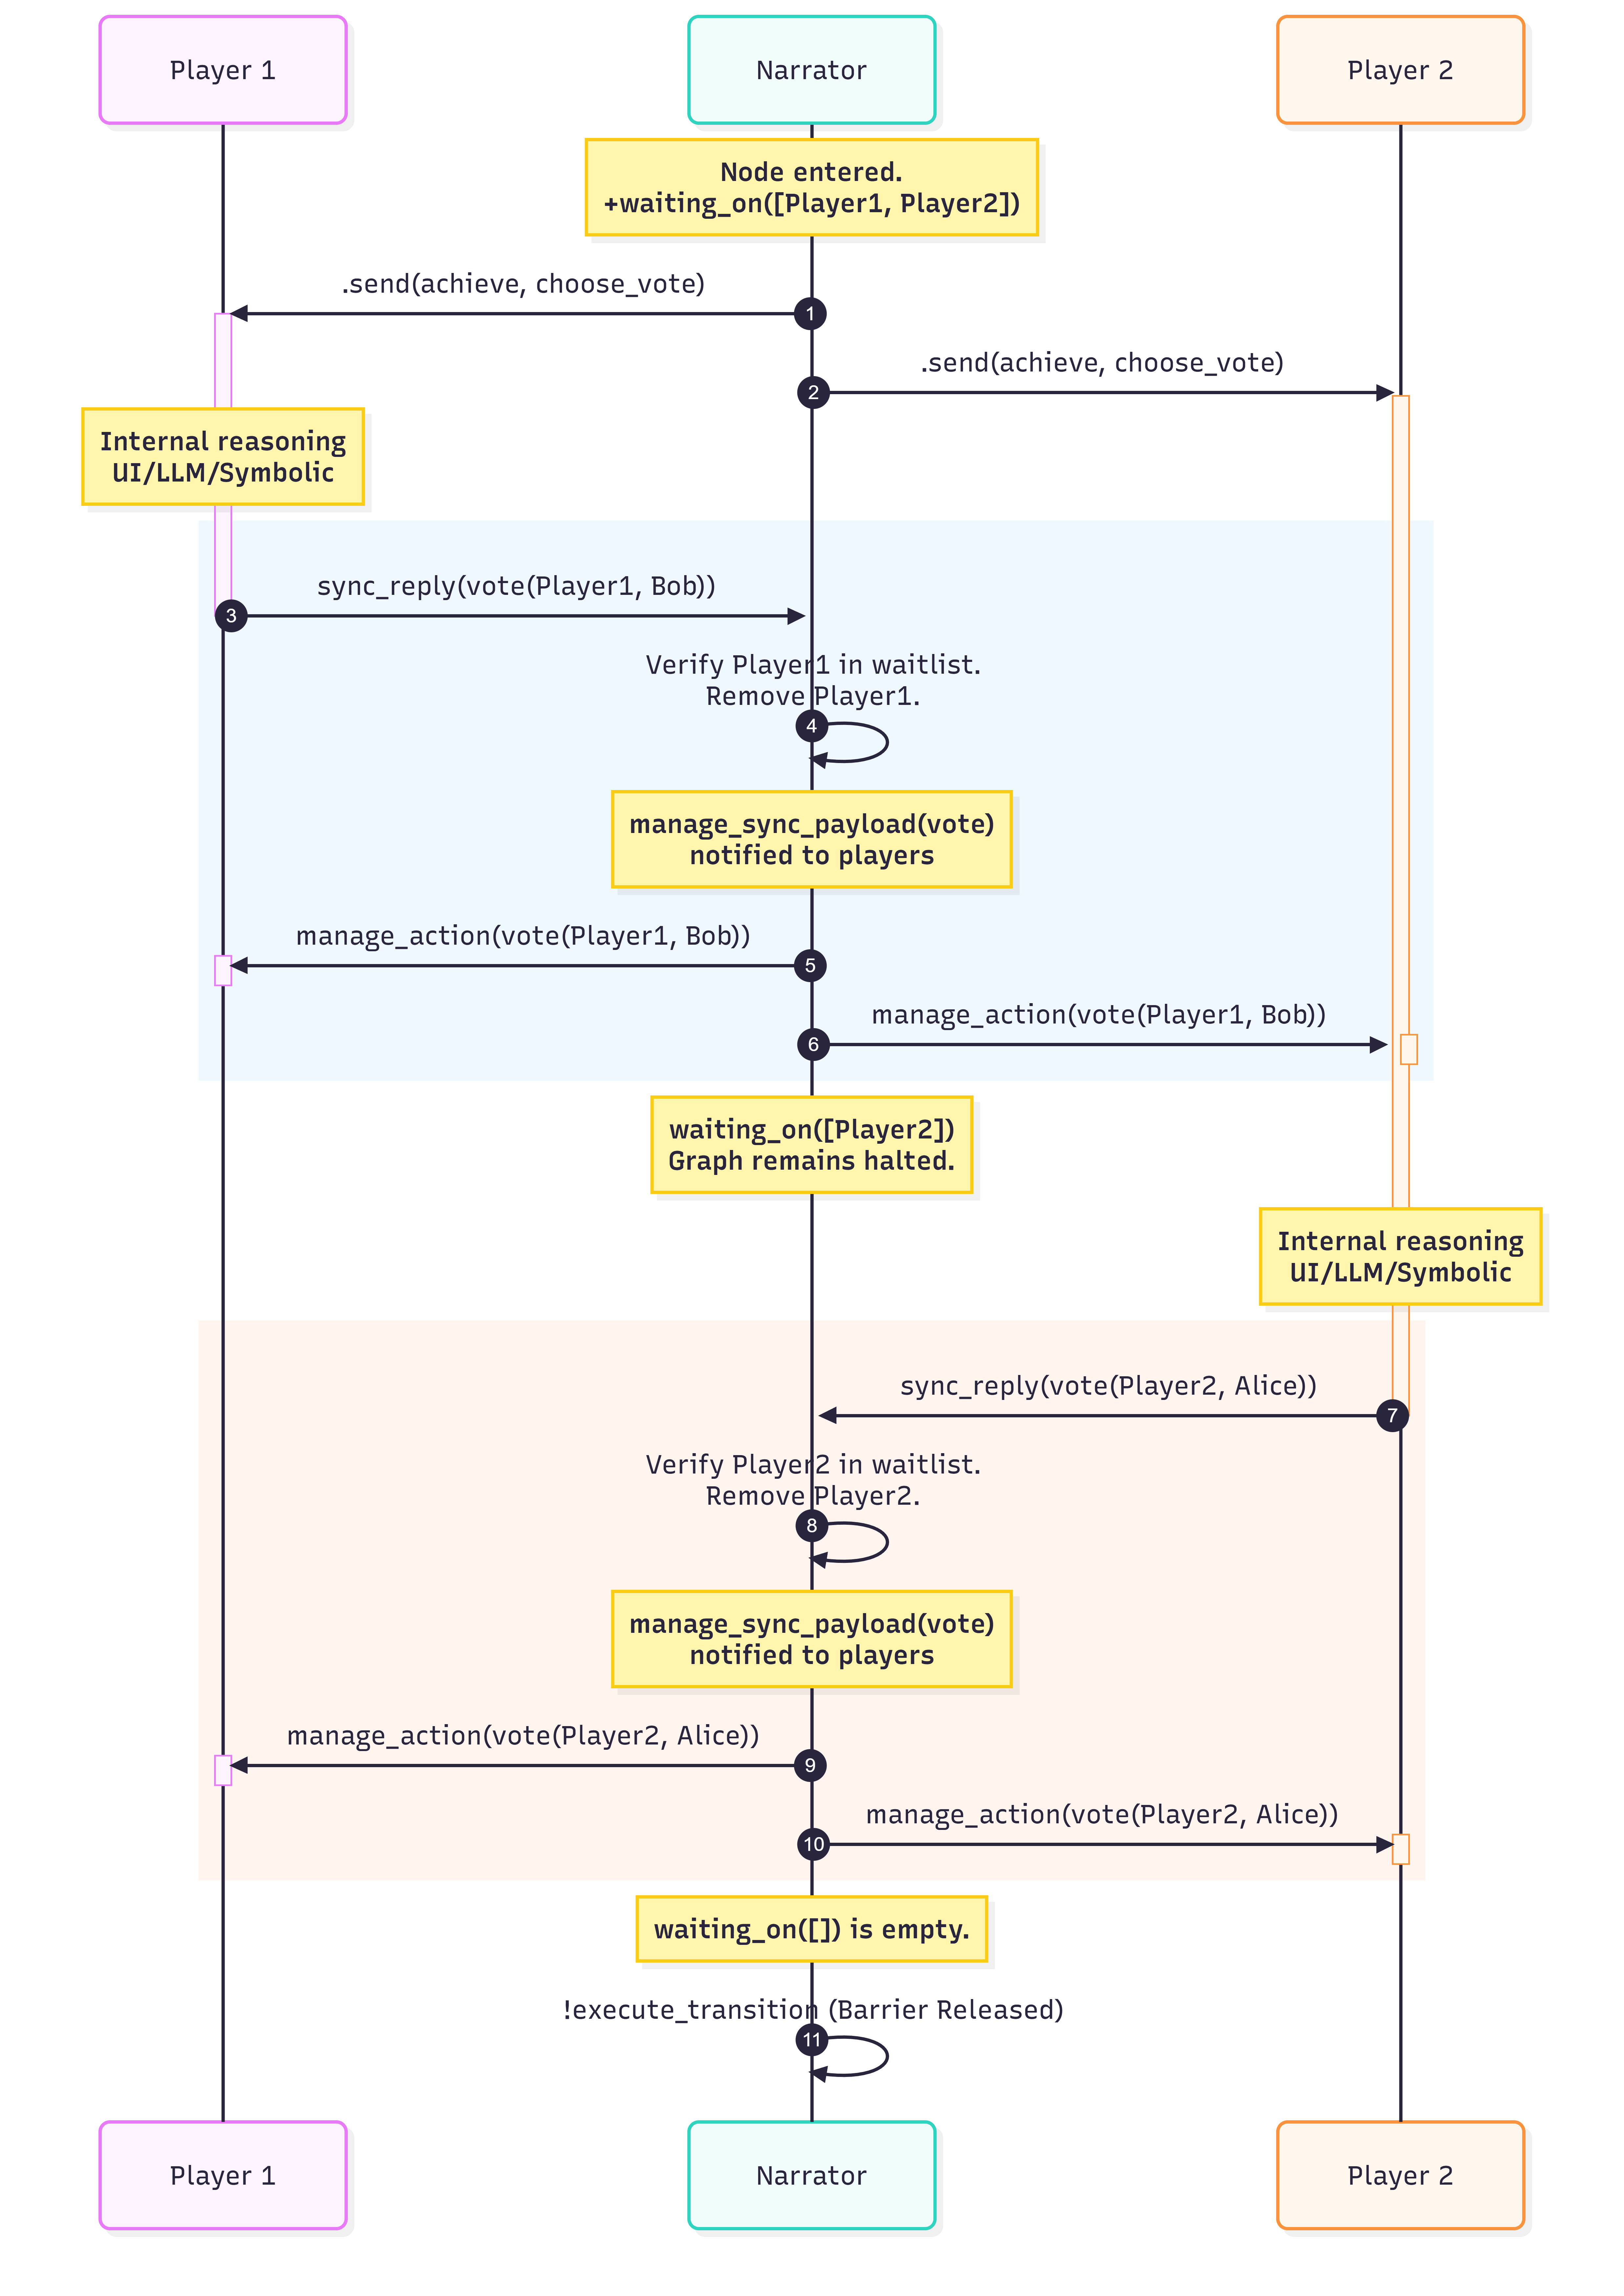
\includegraphics[width=1\textwidth]{images/sync_barrier_diagram.png}
    \caption{Sequence diagram illustrating the resolution of the Synchronization Barrier. The primary objective is to guarantee that the Narrator and all active players ultimately maintain an identical, globally synchronized chronological log of events (e.g., \texttt{choose\_vote}, \texttt{vote(Player1, bob)}, \texttt{vote(Player2, alice)}).}
    \label{fig:sync_sequence}
\end{figure}




\subsection{Phase Execution Examples}
\label{subsec:phase-execution-examples}

While the general transition engine manages the flow of the Game Graph, some specific nodes require the Narrator to execute custom logic to resolve the game state; this section details the \emph{vote counting} and the \emph{speaker selection} practical implementation.

\subsubsection{Vote Counting Mechanism}
The voting counts mechanism is used in particular twice in the game logic :after  the Wolves' nocturnal hunt and the Villagers' daytime execution.
The Narrator triggers either \texttt{count\_hunt\_votes} or \texttt{count\_peasant\_votes}, which collects all the respective vote beliefs; then to ensure reusability, the target's list is unified with a goal-oblivious Prolog rule \texttt{tally\_votes}.


\vspace{1em}
\begin{lstlisting}[frame=single, language=Prolog, caption={The unified vote counting logic and the \emph{Peasant vote} resolution plan; after the count, \texttt{tie\_count\_village(TieCount)} indicates if the vote was a tie, and \texttt{max\_victim\_village(MaxVictim)} defines the eventual victim of the vote.}, label={lst:vote_counting}]
tally_votes(VoteList, TieCount, MaxVictim)  
    :-.setof(V, .member(V, VoteList), UniqueVictims)          
    & .findall(vote_count(C, V),
        ( .member(V, UniqueVictims) 
        & .count(.member(V, VoteList), C)), 
        Tally)
    & .max(Tally, vote_count(MaxCount, MaxVictim))            
    & .count(
        .member(vote_count(MaxCount, _), Tally), 
        TieCount). 

+!count_peasant_votes
    <-  .findall(V, vote(_, V), AllVotes);
        ?tally_votes(AllVotes, TieCount, MaxVictim);
        
        //save results as beliefs
        +tie_count_village(TieCount); 
        +max_victim_village(MaxVictim);
        
        !execute_transition.
\end{lstlisting}

The \texttt{tally\_votes} rule then processes the list through as shown in Listing \ref{lst:vote_counting}:
\begin{enumerate}
    \item It extracts a set of all unique targeted victims.
    \item It counts the occurrences of each target within the vote list.
    \item It define the highest vote count and the specific victim who received it.
    \item It checks how many targets receive the maximum number of votes.
\end{enumerate}

The count's results are then saved as explicit beliefs: they will be automatically used by the Jason Interpreter to define wich edges are valid, during the explicitly called transition to the  next phase. 

\subsubsection{Speaker Selection Implementation}
\label{subsubsec:speaker_selection}

During the \texttt{start\_discussion\_round} phase, players explicitly tell the Narrator their intent to speak based on their internal reasoning. The Narrator then chooses (simulating a natural conversation, while avoiding monopolization) from those volunteers a Player that hold the floor.

Upon entering the \texttt{evaluate\_intents\_to\_speak} node, the Narrator collects all volunteer intents and categorizes them to ensure a responsive and logically coherent dialogue. These categories carry the following semantic meanings:

\begin{itemize}
    \item \textbf{\texttt{yes} (\texttt{normal}):} The player is an AI (symbolic or LLM) that wants to speak.
    \item \textbf{\texttt{privileged}:} Human players with intents to speak. Prioritizing their inputs augment human interactivity and overall game enjoyability.
    \item \textbf{\texttt{targeted}:} Specific player who was the direct topic of the preceding speech in the current round; it has a higher chance to be choosen to speak, to ensure the  possibility to defend  itself from previous accusations.
\end{itemize}
To enforce a dynamic dialogue, the Narrator explicitly filters out the \texttt{last\_speaker} from all eligibility lists, ensuring no player can speak twice in a row in the same round. 

\vspace{1em}
\begin{lstlisting}[frame=single, language=Prolog, caption={The priority cascade logic for speaker selection, with 4 rules evaluated top to bottom. The arguments needed are list of the players with intent to speak, subdivided in Privileged, Targeted, Normal}, label={lst:speaker_selection}]

// Priority 1: Privileged volunteer (Human players)
+!pick_candidate(Privileged, _, _, Speaker) 
    : Privileged \== []
    <- .shuffle(Privileged, [Speaker|_]).

// Priority 2: Targeted player (P=0.25)
+!pick_candidate(_, [Speaker], _, Speaker) 
    : .random(R) & R <= 0.25.

// Priority 3: Normal volunteer (AI agents)
+!pick_candidate(_, _, Normal, Speaker) 
    : Normal \== []
    <- .shuffle(Normal, [Speaker|_]).

// Priority 4: Targeted player
+!pick_candidate(_, [Speaker], _, Speaker).
\end{lstlisting}

If no one volunteers (meaning both the normal and privileged lists are empty), the Narrator immediately aborts the discussion round; otherwise, the selection process follows a priority cascade defined by the\texttt{pick\_candidate} plans, detailed in Listing \ref{lst:speaker_selection}:

\begin{enumerate}
    \item \textbf{Human players :} If any active human player define the intent to speak, sample one randomly. 
    \item \textbf{Right to fight back:} If the previously targeted player wishes to speak, with chances of 25\% it will hold the floor.
    \item \textbf{Random selection:} Select randomly (if any) a Agent driven by its AI, with positive intent to speak.
    \item \textbf{Duty to fight back:} Fallback case, the floor is given to the targeted player by default.
\end{enumerate}

Once a speaker is designated, the Narrator logs them as the new \texttt{last\_speaker}, broadcasts a \texttt{time\_to\_speak} action to all players, and sets up a synchronization barrier waiting specifically for that agent to deliver their speech payload.

\subsection{Logging System}
\label{subsec:logging}

The Narrator manages a centralized \emph{log} to keep a persistent history of the game (the logic is self-contained in the file \texttt{narrator/log\_manager/logger.asl}). Before dispatching any phase transition or action to the agents, the engine internally appends it to this log (with an $O(1)$ complexity, since it is natively implemented as a linked list). 

The list is used in an append-only fashion: new entries are pushed to the head, and entries are never removed, only retrieved when needed\footnote{This inherent inability to cut off past events even if they are no longer useful could theoretically lead to memory-related problems, but in practice, no tests ever reached that critical point.}.

To prevent knowledge leakage (e.g., ensuring a Villager cannot access the Wolves' nocturnal chat), we exploit Jason's native belief annotations. Every entry is tagged with its specific audience. 
To optimize RAM usage and improve readability, the actual list of targets is compressed into global keywords (\texttt{players}, \texttt{wolves}, \texttt{villagers}) when possible before being stored. 

When an agent needs to retrieve a chunk of the log\footnote{The use cases of the retrieval system are explained in Section~\ref{sec:llm}: the log is used to further drive of the \emph{in-context learning} natively implemented by the LLM.}, it can directly query the Narrator: the compressed annotations are expanded back into a list, and the Narrator verifies if the requesting set of players is a valid subset of the entry's audience (if not, the entry is simply ignored). 

This centralized extraction logic prevents the extreme RAM usage that would occur if we maintained separate, parallel logs for every single player in the MAS.

\section{The Player(s)}
\label{sec:players}

The Player Agents within are implemented as \emph{modular BDI shells}, acting as an interface wrapper around a \emph{Reasoner}, whose exact behavior must be implemented by the developer. This architecture cleanly decouples the network communication and state management from the actual decision-making logic.

As illustrated in Figure \ref{fig:agent_interface}, the agent shell exposes two primary interfaces to interact with the environment: a \emph{Decision Execution Interface} and a \emph{State Management Interface}.

\begin{figure}[htpb]
    \centering
    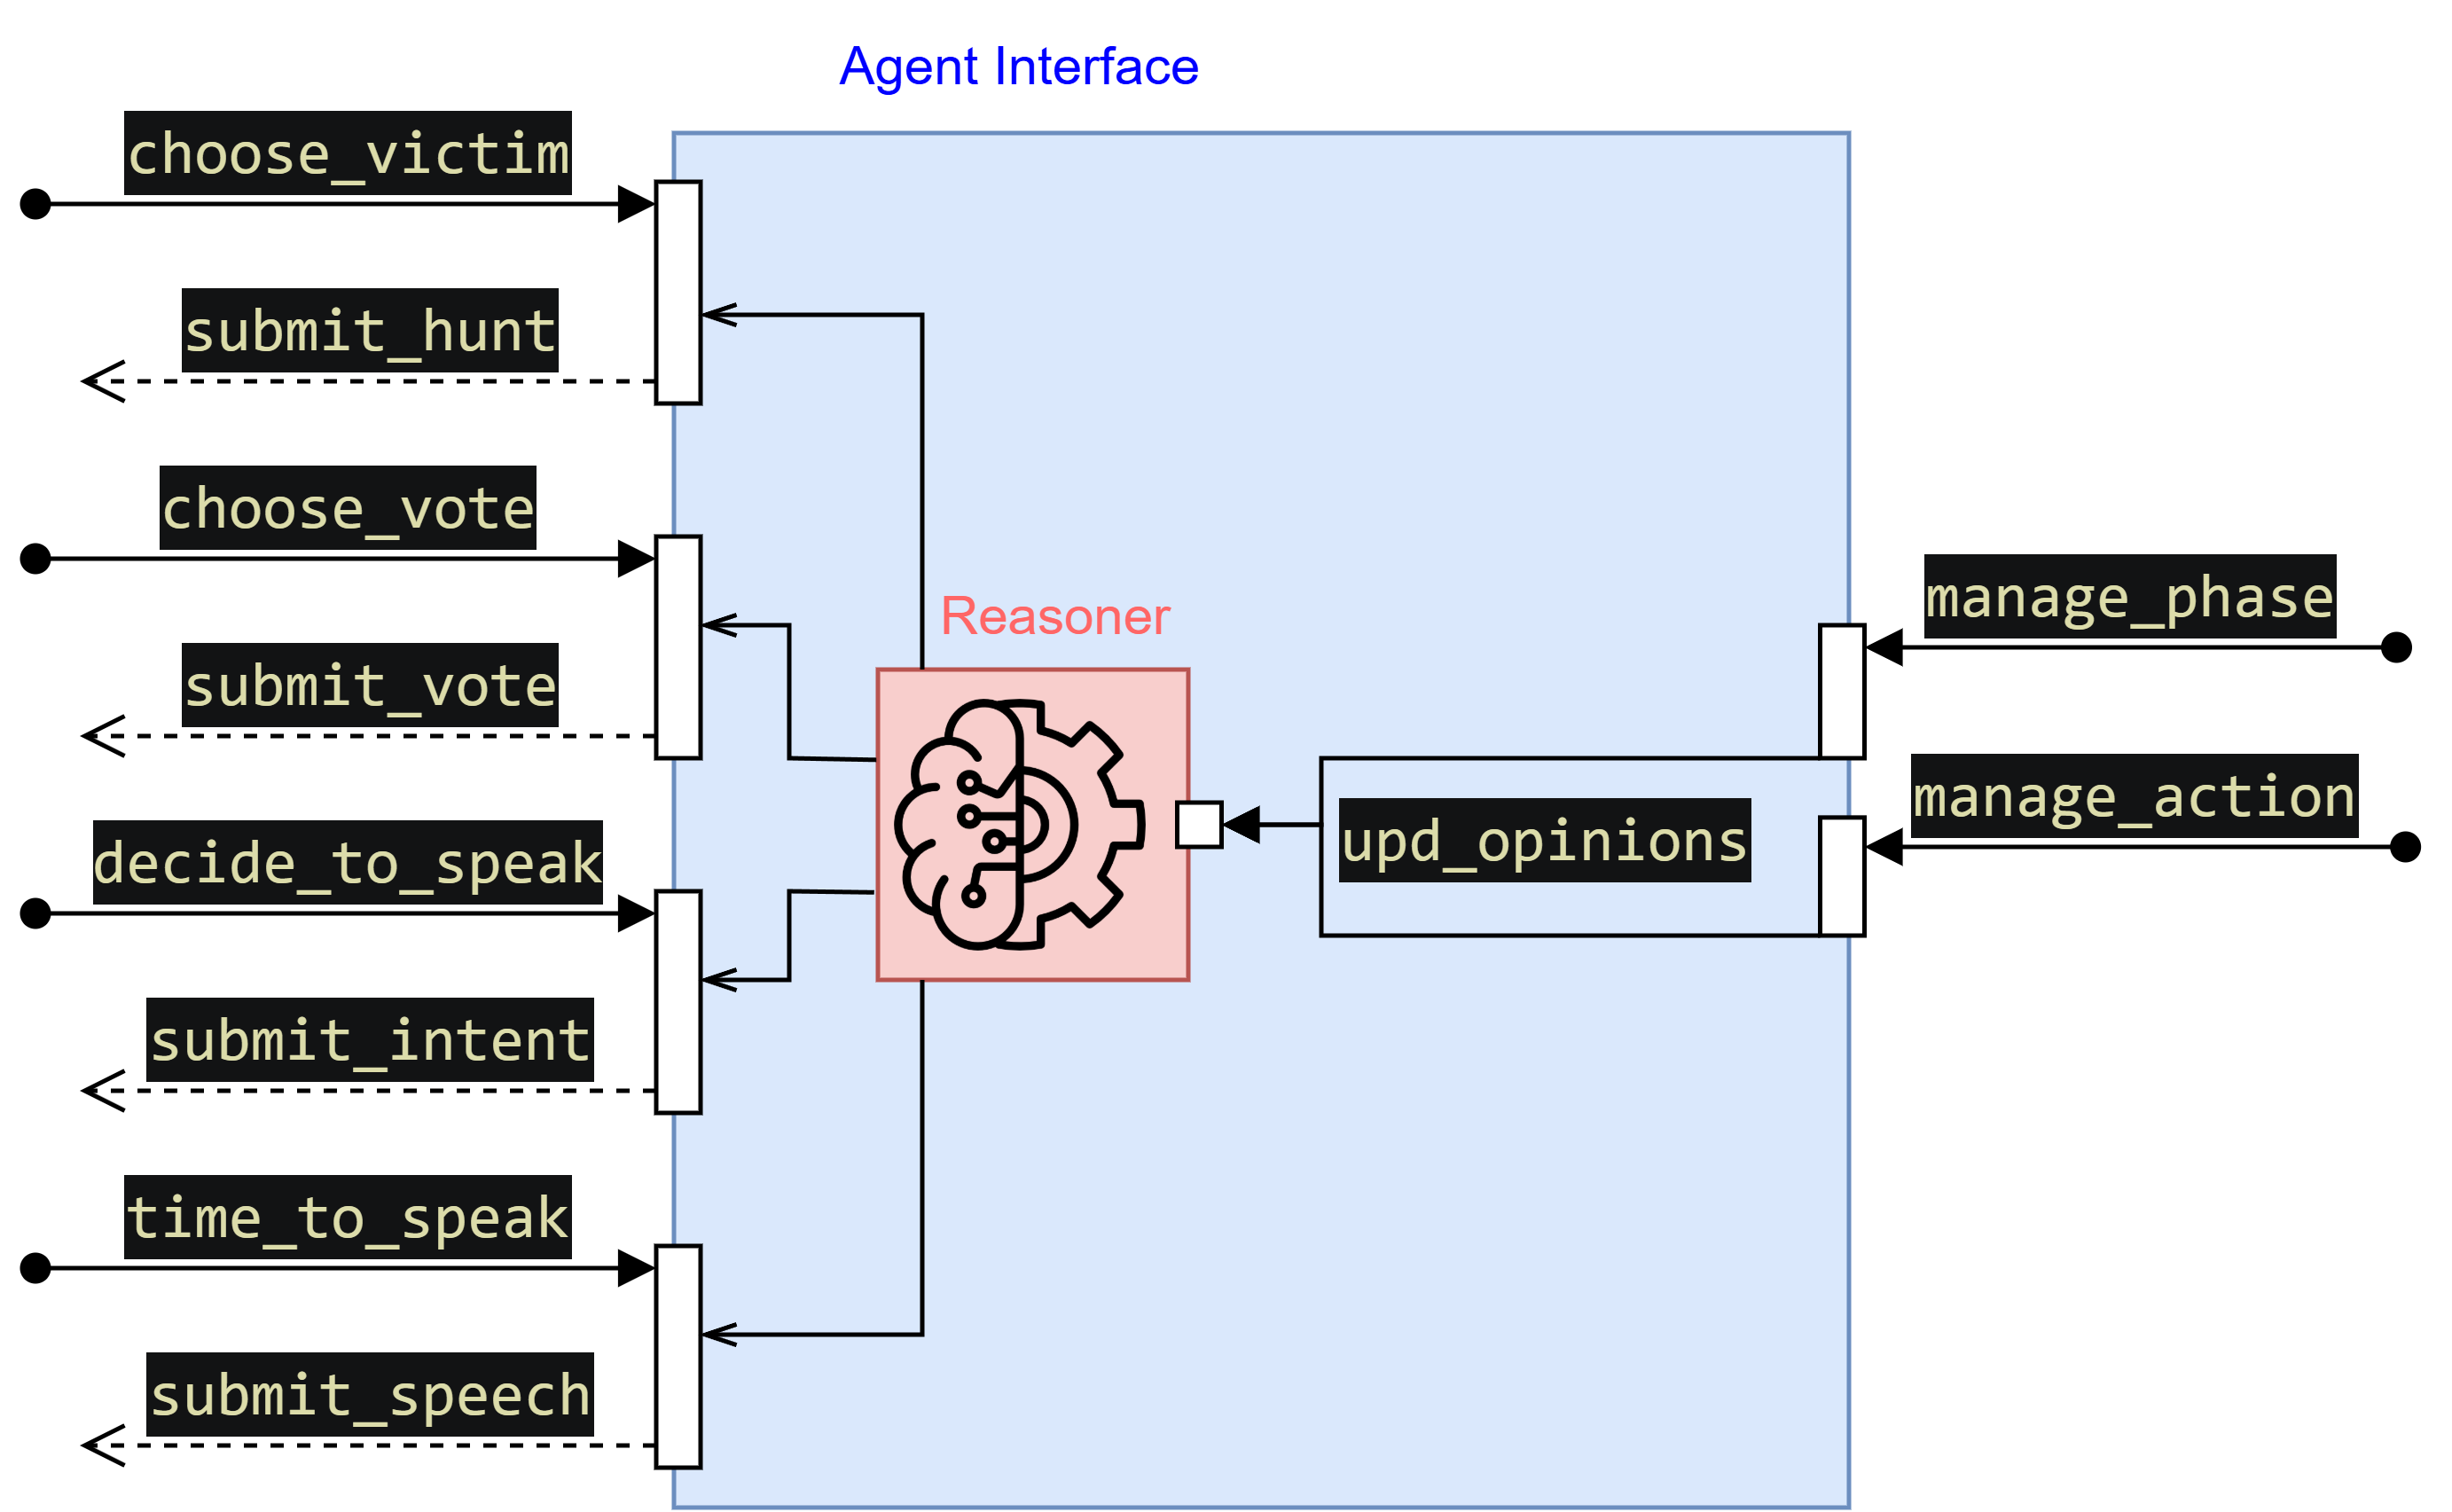
\includegraphics[width=0.8\textwidth]{images/agent_interface.png}
    \caption{Conceptual architecture of the Player Agent, illustrating the decoupling of the fixed network interfaces from the swappable Reasoner logic.}
    \label{fig:agent_interface}
\end{figure}


\paragraph{Decision Execution Interface}
To simplify the interaction protocol, the interface implements a closed-world assumption: every choice must be drawn from an explicitly finite domain. The execution shell must integrate at least 4 plans:
\begin{itemize}
    \item \texttt{choose\_victim}\footnote{The \texttt{choose\_victim} plan is only required if the player holds a \textbf{wolf} role. For standard villagers, the absence of this plan raises no runtime errors, as the Narrator will never explicitly inject this goal for them.} and \texttt{choose\_vote}: Must select  a currently alive player.
    \item \texttt{decide\_to\_speak}: Resolves to a standard intent\footnote{During the resolution phase, the Narrator dynamically casts the a intent into its \texttt{targeted} classification, to properly enforce the discussion phase's speech hierarchy.} (\texttt{yes} or \texttt{no}), or a special \texttt{privileged} flag specifically reserved for human players.
    \item \texttt{time\_to\_speak}: Produces a compound \texttt{speech(Message, Performative(Target))} action. The \texttt{Message} is a textual string, while the \texttt{Performative} must be selected from an enumerated set of valid speech acts (\texttt{accuse}, \texttt{defend}, \texttt{suspect}, \texttt{agree}, \texttt{interrogate}, or \texttt{deflect}) directed at an alive player.
\end{itemize}

When the Narrator inject the agent of its turn, the interface queries the underlying Reasoner to obtain behavior within these rigid boundaries. Once generated, the shell wraps the output into the corresponding submission action to synchronize with the Narrator. 

Furthermore, the architecture could require also a \texttt{guess\_performative} plan, which attempts to extract a valid \texttt{Performative(Target)} tuple from raw textual input if the explicit speech act is missing (further detailed in Section \ref{sec:speech_act_misalignment}).

To prevent temporal misalignment and race conditions across the distributed system, all decisions are strictly dispatched back to the Narrator using the \texttt{sync\_reply(...)} functor (already detailed in Subsection~\ref{subsec:sync-barrier}), as demonstrated in Listing \ref{lst:sync_reply_example}: this implementative choice completely disregard direct communication P2P.

\vspace{1em}
\begin{lstlisting}[frame=single, language=Prolog, caption={An example of a submission helper enforcing synchronization by exclusively replying to the Narrator.}, label={lst:sync_reply_example}]
+!submit_vote(Target) 
  <-.my_name(Me);
    .send(narrator, achieve, sync_reply(vote(Me, Target))).
\end{lstlisting}



\paragraph{State Management Interface} It guarantees the agent's reactivity to the environment. It relies on two passive listener plans: \texttt{manage\_phase} and \texttt{manage\_action}: the goals are injected by the narrator, and the plans does not need to communicate back to the narrator any information (in fact, most of the time the delivered action/phases are ignored altogether). 

Their purpose is to process (mainly by triggering updates to the UI) the incoming events broad casted from the narrator,  and subsequently invoke the \texttt{upd\_opinions(Sender, Action)} hook defined in the Reasoner. As shown in Figure \ref{fig:agent_interface}, this specific hook acts as the bridge to the Reasoner, defining explicit events to update its Belief Base and ensuring the cognitive engine is continuously supplied with an accurate, up-to-date representation of the game's state.


It should be noted that the provided agent interface diagram represents a conceptual simplification. The actual implementation within the Jason environment also integrates extensive conditional hooks to a Graphical User Interface (GUI). When an active UI is present, both the state changes and the decisions trigger corresponding visual updates to dynamically reflect the agent's internal state and actions to the human observer (Section \ref{sec:ui}).


\subsection{Setup and Initialization}
\label{subsec:player-setup}

The orchestration of the simulation begins strictly within the configuration file, \texttt{werewolf.jcm}. To maximize modularity and code reuse, every player in the game is instantiated from a single, universal entry point: the \texttt{players/init\_player.asl} file.

\begin{verbatim}
    agent bob : init_player.asl {
        instances : 1
        beliefs: iam(wolf), reasoner(human)
    }
\end{verbatim}

Within the configuration file, each agent is assigned two mandatory initial beliefs to define their core parameters:
\begin{itemize}
    \item \textbf{\texttt{iam(Role)}:} Dictates their team affiliation, defining them as either a \texttt{wolf} or a \texttt{villager}.
    
    \item \textbf{\texttt{reasoner(Type)}:} Define the cognitive engine, natively accepting values such as \texttt{human}, \texttt{llm}, or \texttt{symbolic}.
\end{itemize}

Upon initialization, the agent executes the \texttt{+!configure\_player} plan, which evaluates these assigned beliefs and orchestrates a multi-step boot sequence. First, the agent resolves the requested cognitive engine via \texttt{+!resolve\_reasoner}; this step introduces robust fallback logic, such as automatically degrading an \texttt{llm} reasoner to a \texttt{symbolic} one if the LLM is disabled. Next, the system configures the appropriate UI bindings (active/spectator, or none at all).

The agent's structural assembly is then handled by a native Jason routing plan, \texttt{+!load\_modules(Role, ActiveReasoner)}; by using the  Jason's \texttt{.include} directives it dynamically inject the precise \texttt{.asl} modules required by the player.

Once the specialized logic and the universal wrappers (statically included at the head of the file) are fully assembled, the agent executes \texttt{+!cleanup\_boot\_memory} to remove all obsolete plans and beliefs (such as those just activated during initialization, or hooks not used by the newly constructed agent).

\paragraph{Easy configuration}
This modular inclusion pattern ensures that the system remains highly scalable and configurable: it is possible to freely adjust the total number of agents, redefine their roles, or completely swap their underlying reasoning engines by exclusively tinkering with the \texttt{werewolf.jcm} configuration file, all without needing to alter any internal Jason code.



\subsection{Personality and Moods (Jason-Pro)}

To model complex social dynamics, the simulation integrates a variation of the \texttt{vesna.ProAgent} architecture, an extension of the standard Jason engine whose original implementation and details can be found at \cite{vesna_pro_toolkit}. By defining a player with a specific ``temper'', it is possible to fundamentally alter its decision-making process without rewriting the underlying AgentSpeak logic. 

\paragraph{Architectural changes} 
In the original \texttt{ProAgent} implementation, the affective state was encapsulated entirely within the Java architectural layer, since it was only utilized as a hidden heuristic for intention selection. To support the  hybrid reasoning models in the game, the architecture was modified to establish \textbf{bidirectional synchronization} between the Java engine and the AgentSpeak layer.

First, methods were introduced to continuously expose the agent's real-time temper to the AgentSpeak belief base, enabling synchronized updates to the User Interface (section \ref{sec:ui}).

Second, while the original engine strictly managed mood updates via static plan annotations such as $$\texttt{@plan\_example[temper([paranoia(0.8)]), effects([stress(-0.3)[mood]])]} $$ new internal actions were added to allow the Jason agent to explicitly overwrite these values. This ensures that the LLM reasoning engine can actively mutate the agent's emotional states in real time in response to external actions and dynamic game events.

Furthermore, to maintain a notation consistent with the \emph{traits} implemented (subsection \ref{subsec:first_order_beliefs}), the domain of both the temper's states and personality values was shifted from the original $[0, 1]$ to $[-1, 1]$.

\paragraph{Personality definition} The cognitive profile is injected directly during the initialization phase within the \texttt{werewolf.jcm} configuration file; within this new architecture, player configuration is thus a direct upgrade of the one defined previously:

\begin{verbatim}
    agent alice : init_player.asl {
        instances : 1
        ag-class: vesna.ProAgent
        temper: temper( 
            paranoia(-0.8), 
            individualism(0.9), 
            stress(0)[mood], 
            exposure(0.5)[mood] )
        strategy: most_similar
        beliefs: iam(wolf), reasoner(llm)
    }
\end{verbatim}

The \texttt{ag-class} directive overrides the default Jason architecture, linking the agent to the custom Java-based affective engine. The \texttt{temper} definition establishes the agent's baseline psychological profile. It distinguishes between static personality traits (\texttt{paranoia(-0.8)}, \texttt{individualism(0.9)}) and dynamic emotional states via the \texttt{[mood]} annotation (\texttt{stress(0)}, \texttt{exposure(0.5)}). 
Finally, the \texttt{strategy: most\_similar} parameter instructs the agent's intention selection to execute the plan whose affective requirements most closely align with the agent's current temper.




\subsection{Epistemic Beliefs as Long-Term World Model}
\label{subsec:first_order_beliefs}

While the \texttt{vesna.ProAgent} architecture is utilized to model the players' internal states (\textbf{self-awareness}), a formal method is still required to maintain a dynamic, long-term, and subjective representation of the external ``world`` (in the context of the game, the other players).

To address this requirement, the implemented solution employs an explicit trait system to model an agent’s \textbf{first-order epistemic beliefs} regarding its peers\footnote{While modeling higher-order beliefs is theoretically possible within the game's context and architecture, this approach was abandoned to prevent a combinatorial explosion in the dimensionality of the belief matrix, which is already sparse by design (as discussed in Section \ref{sec:results}).}.


\paragraph{The \emph{Traits} Matrix}
By assigning specific traits to the other players, the agent effectively generates a dynamic ``belief matrix`` within the its knowledge base. 
The matrix can be visualized explicitly: the rows corresponding to the other players, the columns the specific tracked traits.

\begin{table}[h]
\centering
\begin{tabular}{lccc}
\hline
\textbf{Player} & \textbf{Suspicion} & \textbf{Utility} & \textbf{Influence} \\
\hline
Alice & 0.8 & 0.5 & 0.9 \\
Bob & -0.4 & 0.2 & - \\
Charlie & - & -0.7 & 0.2 \\
Arthur & -0.9 & 0.8 & -0.5 \\
Bella & -0.8 & 0.6 & 0.1 \\
Caleb & 0.7 & - & 0.4 \\
David & - & 0.4 & 0.8 \\
Eve & - & 0.9 & 0.7 \\
Frank & - & -0.5 & - \\
Grace & 0.9 & -0.8 & 0.3 \\
Heidi & 0.6 & 0.3 & 0.5 \\
Ivan & 0.4 & 0.1 & -0.2 \\
Judy & -0.6 & 0.7 & - \\
Kevin & - & 0.5 & 0.6 \\
Leo & 0.0 & 0.0 & - \\
\hline
\end{tabular}
\caption{Player Trait Matrix: the lazy initialization ensures that empty cells contain a value when they will be used.}
\end{table}

This internal representation enables the AgentSpeak interpreter to identify the most suitable target players using customizable heuristics. An application of this approach is detailed in Section \ref{subsec:symbolic-reasoner}, which introduces a symbolic reasoner that directly queries this belief matrix to drive the agent's decision-making process.

\paragraph{Implemented Traits}
The trait framework is designed to be highly modular, allowing to append new heuristics freely without any particular constraint. In the current implementation, each agent keep a matrix where each peer is characterized by 3 traits:

\begin{itemize}
    \item \textbf{Suspicion (Villager specific):} A low level indicates the target is believed to be innocent and trustworthy, while a higher value indicates a strong belief that the target is a wolf.
    \item \textbf{Threat (Wolf specific):} A low level means the target is ignoring the pack or poses no danger, whereas a higher value indicates they are actively attacking the wolves.
    \item \textbf{Utility (Universal):} Evaluates strategic usefulness: a low level defines the target as an obstacle, while a bigger value implies they are actively helpful to the agent's goals.
    \item \textbf{Influence (Universal):} Evaluates social capital: a low level means the target is losing credibility and does not show leadership, while a bigger value denotes that they are highly persuasive and leading the game logic.
\end{itemize}


\subsubsection{Lazy Initialization and Consistency}
To optimize memory usage and accurately simulate initial social uncertainty, the belief matrix employs a lazy initialization implementation. If an agent attempts to query a trait for a specific player that has not yet been formed, the system dynamically generates it on the fly. Rather than starting from an absolute zero, a small amount of Gaussian noise is added to mirror the ``prior knowledge'' that players might possess\footnote{From an implementation perspective, adding random noise to each player's world model ensures stochasticity. This prevents the inherent determinism of a symbolic engine from causing agents to form identical beliefs and, consequently, show uniform behavior.}. 

To ensure mathematical consistency across the reasoning cycle and the UI rendering, all trait values are strictly clamped within the $[-1, 1]$ interval and rounded to two decimal places.

\begin{lstlisting}[frame=single, language=Prolog, caption={Implementation of trait management defined in \texttt{players/first\_order\_beliefs/traits.asl}. The code features lazy initialization of undefined traits using Gaussian noise to introduce stochasticity, alongside an atomic update plan that seamlessly queries (initializing if necessary) and modifies the belief by a given delta.}, label={lst:trait_management}]
    //ensure value in range [Min, Max]
    //define DP decimal places
    clamp(Val, Clamped)
        :-  setting(trait_bounds(Min, Max, DP))
        &   Factor  = 10**DP
        &   TempVal = math.max(Min, math.min(Max, Val))
        &   Clamped = math.round(TempVal * Factor) / Factor.
    
    //MAGIC NUMBERS to add gaussian noise
    add_noise(Mean, StdDev, ClampedResult)
        :-  .random(U1) &   .random(U2)
        &   RealU1 = math.max(0.0001, U1)
        &   Z0 = math.sqrt(-2.0 * math.log(RealU1)) 
               * math.cos(6.28318530718 * U2)
        &   RawVal = Mean + (Z0 * StdDev)
        &   clamp(RawVal, ClampedResult).
    
    //lazy initialization, if not exists
    +?trait(Player, Attr, Value) 
        :   not trait(Player, Attr, _)
        &   setting(trait_bounds(Min, Max, _))
        &   setting(trait_init_noise(StdDev))
        &   add_noise((Min + Max) / 2.0, StdDev, Value)
        <-  +trait(Player, Attr, Value).
    
    //else, simple read
    +?trait(Player, Attr, Value) 
        :   trait(Player, Attr, Value).

    //plan to update a trait
    @upd_trait[atomic]
    +!upd_trait(Player, Attr, Delta)
        <-  ?trait(Player, Attr, CurrentVal);
            ?clamp(CurrentVal + Delta, NewVal);
            .abolish(trait(Player, Attr, _));
            +trait(Player, Attr, NewVal).    
\end{lstlisting}

Furthermore, this dynamic architecture offers high scalability during runtime: theoretically, entirely new trait categories could be defined and queried for a player at any moment without requiring reconfiguration\footnote{However, dynamically introducing new trait types during runtime was intentionally restricted in the final implementation to enforce a ``closed-world assumption''. This constraint is necessary, again, to prevent a combinatorial explosion in the belief matrix's dimensionality.}.



\subsection{Symbolic Reasoner (Jason-Pro)}
\label{subsec:symbolic-reasoner}

With the foundational architecture established, we can define the first type of cognitive engine required for a fully autonomous Multi-Agent System (MAS) simulation. As illustrated before in Figure \ref{fig:agent_interface}, the reasoner must exhibit two primary capabilities: it must continuously store and update information within its internal ``world model``, and it must retrieve this data to govern the agent's decision-making behavior.

As previously defined, this internal world representation is composed of the agent's affective ``self-awareness'' (its temper and personality) and its first-order epistemic beliefs regarding other players. Together, these internal states effectively define the player as a deterministic state machine.

\begin{figure}[H]
    \centering
    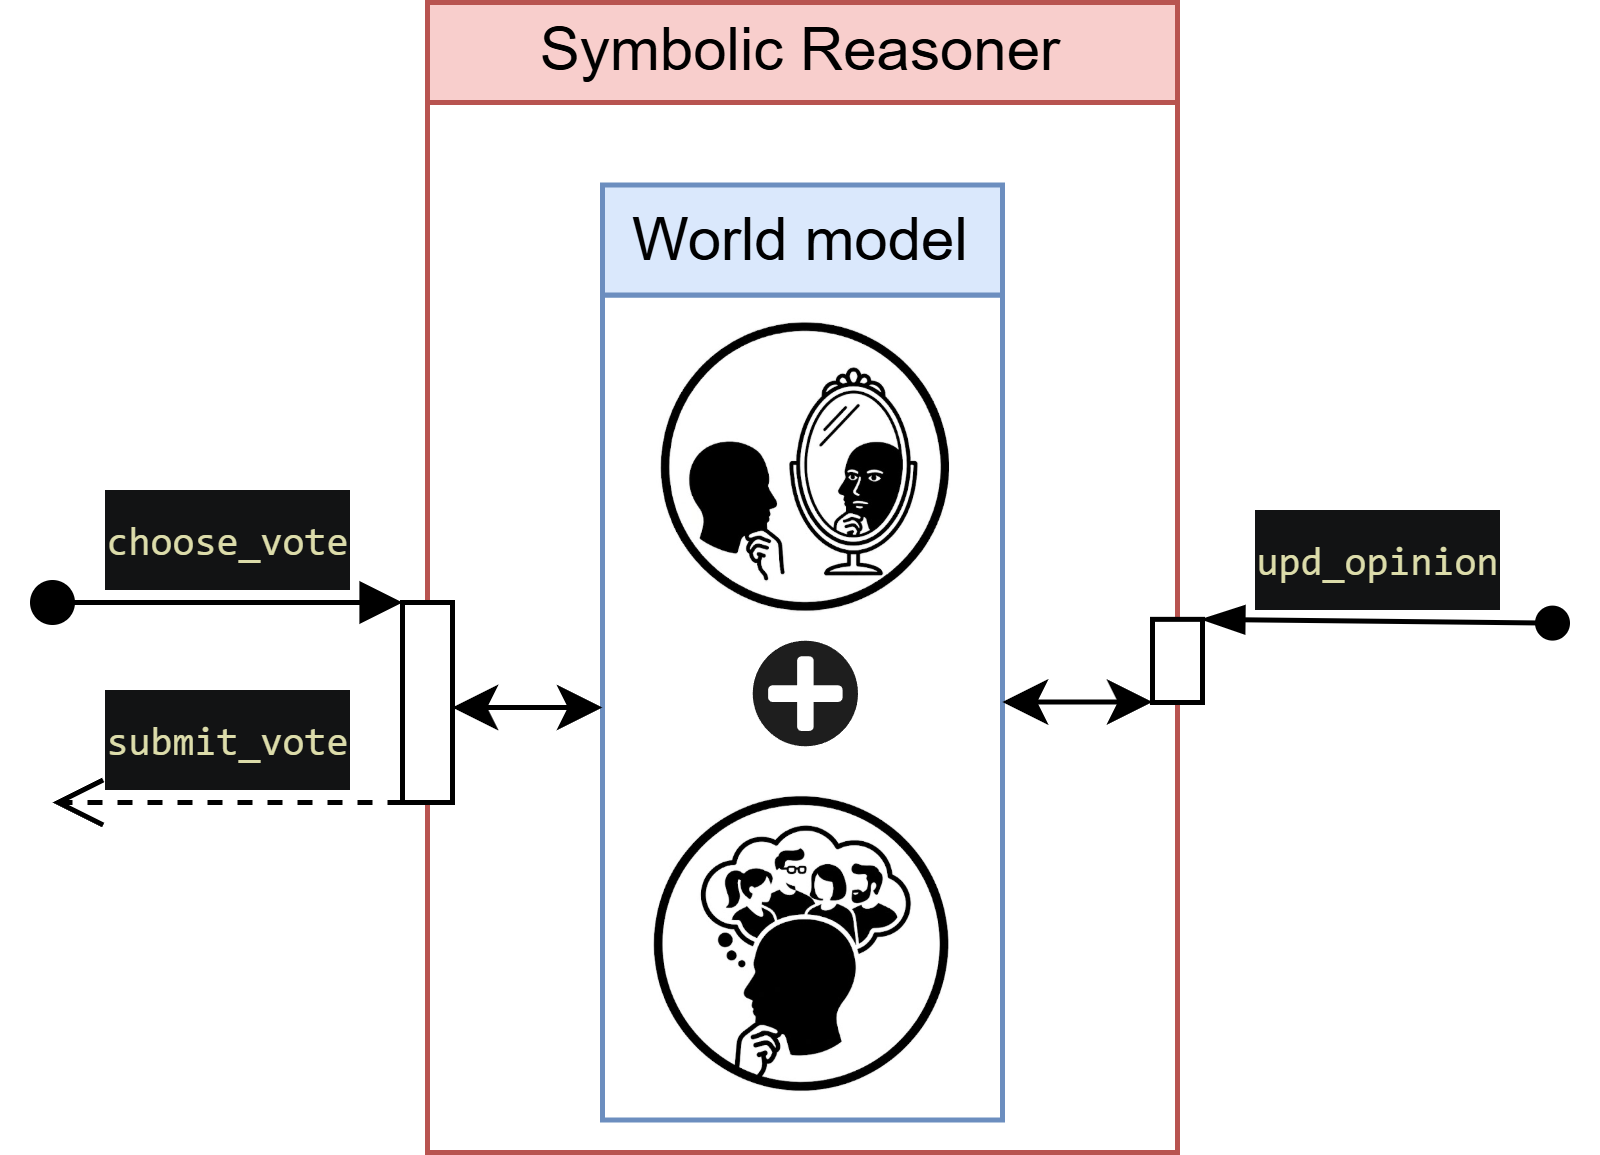
\includegraphics[width=0.6\textwidth]{images/symbolic_reasoner/simplified_symbolic_reasoner.png}
    \caption{Conceptual architecture of the Symbolic Reasoner: at an abstract level, it acts as an interface to query and update the agent's internal world model, which comprises both its \emph{self-awareness} and \emph{first-order epistemic beliefs} about others.}
    \label{fig:symbolic_reasoner}
\end{figure}

The technical implementation of the reasoner's interface, which serves as the execution wrapper for accessing and modifying this internal state, is defined in \texttt{reasoners/symbolic/interface.asl}.

\paragraph{Log retrieval (and Caching)}
For a finer representation of the most recent events, the players can also query the \emph{Narrator} to obtain the last log chunk. Since multi-agent communication in Jason natively brings asynchronous overhead (by forcing the de-scheduling of the active intention), it was also needed to ensure a correct \emph{caching architecture} of the chunks.

When an agent requests a log sequence using the \texttt{+!fetch\_log\_block} plan and the \texttt{cache\_if\_possible} flag, the retrieved data is stored locally in its belief base. A locking mechanism prevents redundant network calls from concurrent requests. To ensure data consistency without continuous polling, the narrator actively invalidates this cache whenever new events modify the historical record.

This logic is integrally implemented in the file \texttt{log\_getter/getter.asl}.

\paragraph{Role-Specific Strategies}
While the player's interface provides a standard execution wrapper, the symbolic reasoner requires role-specific logic. As explained in Subsection \ref{subsec:player-setup},in the player initialization is dynamically loaded the appropriate strategy module (\texttt{strategies/wolf.asl} or \texttt{strategies/villager.asl}). This specialization is crucial, as the two roles exhibit fundamentally different cognitive plans and affective heuristics in response to the exact same game events.


\subsubsection{Updating the Internal State}
As previously discussed, the Reasoner implements its reactivity to events by defining execution plans implementing the \texttt{upd\_opinions(event)} goal. To fully use the capabilites of the \texttt{ProAgent} implementation,is needed to define \textbf{a pool of candidate plans} for each event, as demonstrated in Listing \ref{lst:opinion_pool_example}.

\begin{lstlisting}[frame=single, language=Prolog, caption={Example of the Villager's plan pool used to react to a player's intent to speak. The java engine selects the most suitable reaction based on the agent's temper.}, label={lst:opinion_pool_example}]
@p1[ temper([exposure(0.7)[mood], stress(-0.2)[mood]]), 
     effects([exposure(-0.1)[mood]]) ]
+!upd_opinions(Speaker, intent_to_speak(yes))
    <-  !upd_trait(Speaker, influence, 0.1).

@p2[ temper([paranoia(0.7), stress(0.4)[mood]]),
     effects([stress(0.05)[mood]]) ]
+!upd_opinions(Speaker, intent_to_speak(yes))
    <-  !upd_trait(Speaker, influence, 0.05);
        !upd_trait(Speaker, suspicion, 0.05).

@p3[ temper([paranoia(0.6), stress(0.5)[mood]]), 
     effects([stress(0.1)[mood]]) ]
+!upd_opinions(Speaker, intent_to_speak(no))
    <-  !upd_trait(Speaker, influence, -0.1);
        !upd_trait(Speaker, suspicion, 0.1).

@p4[ temper([individualism(0.7), paranoia(-0.4)])]
+!upd_opinions(Speaker, intent_to_speak(no))
    <-  !upd_trait(Speaker, influence, -0.15).
\end{lstlisting}

By design of the Jason-Pro extension, the reasoning engine evaluates this candidate pool to dynamically select the optimal plan driven by the agent's current \texttt{temper}; at the same time, it processes also the \texttt{effects(...)} annotation, changing the agent's internal mood and updating its overall self-awareness\footnote{To guarantee unbiased plan selection, it is \textbf{required} that all \texttt{temper([...])} annotations within a pool share the exact same dimensionality, since the engine calculates an unnormalized distance metric; the implementation is explained in \cite{vesna_pro_toolkit}, specifically is defined in the file \texttt{src/vesna/ProAgent.java }}.

\begin{figure}[H]
    \centering
    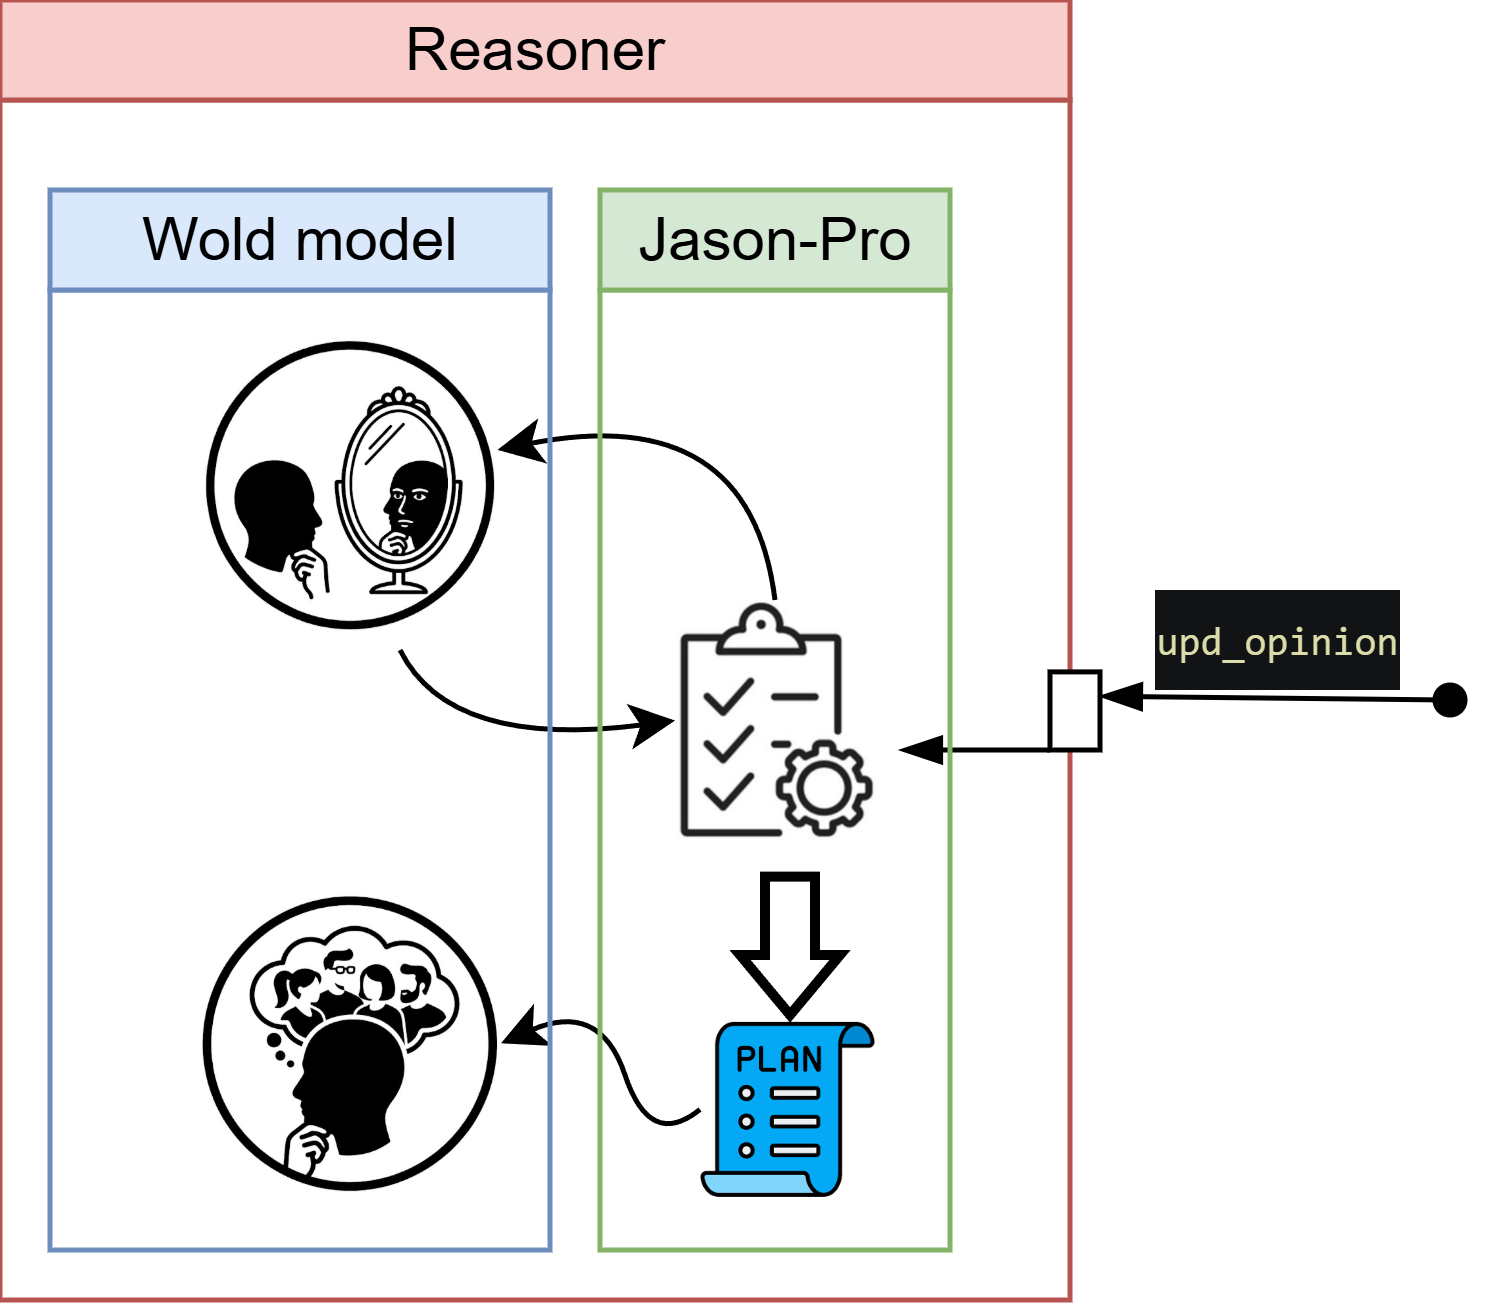
\includegraphics[width=0.6\textwidth]{images/symbolic_reasoner/write_on_symbolic_reasoner.png}
    \caption{Execution pipeline for state updates: external events trigger \texttt{upd\_opinion}, prompting the Jason-Pro engine to evaluate the candidate pool, select a specific plan, and subsequently update both its self-awareness and first-order epistemic beliefs.}
    \label{fig:symbolic_reasoner_write}
\end{figure}

Once selected the plan, executing it applies precise quantitative shifts to the target players' traits, changing the agent's internal belief matrix.


\subsubsection{Querying the Internal State}

\begin{figure}[H]
    \centering
    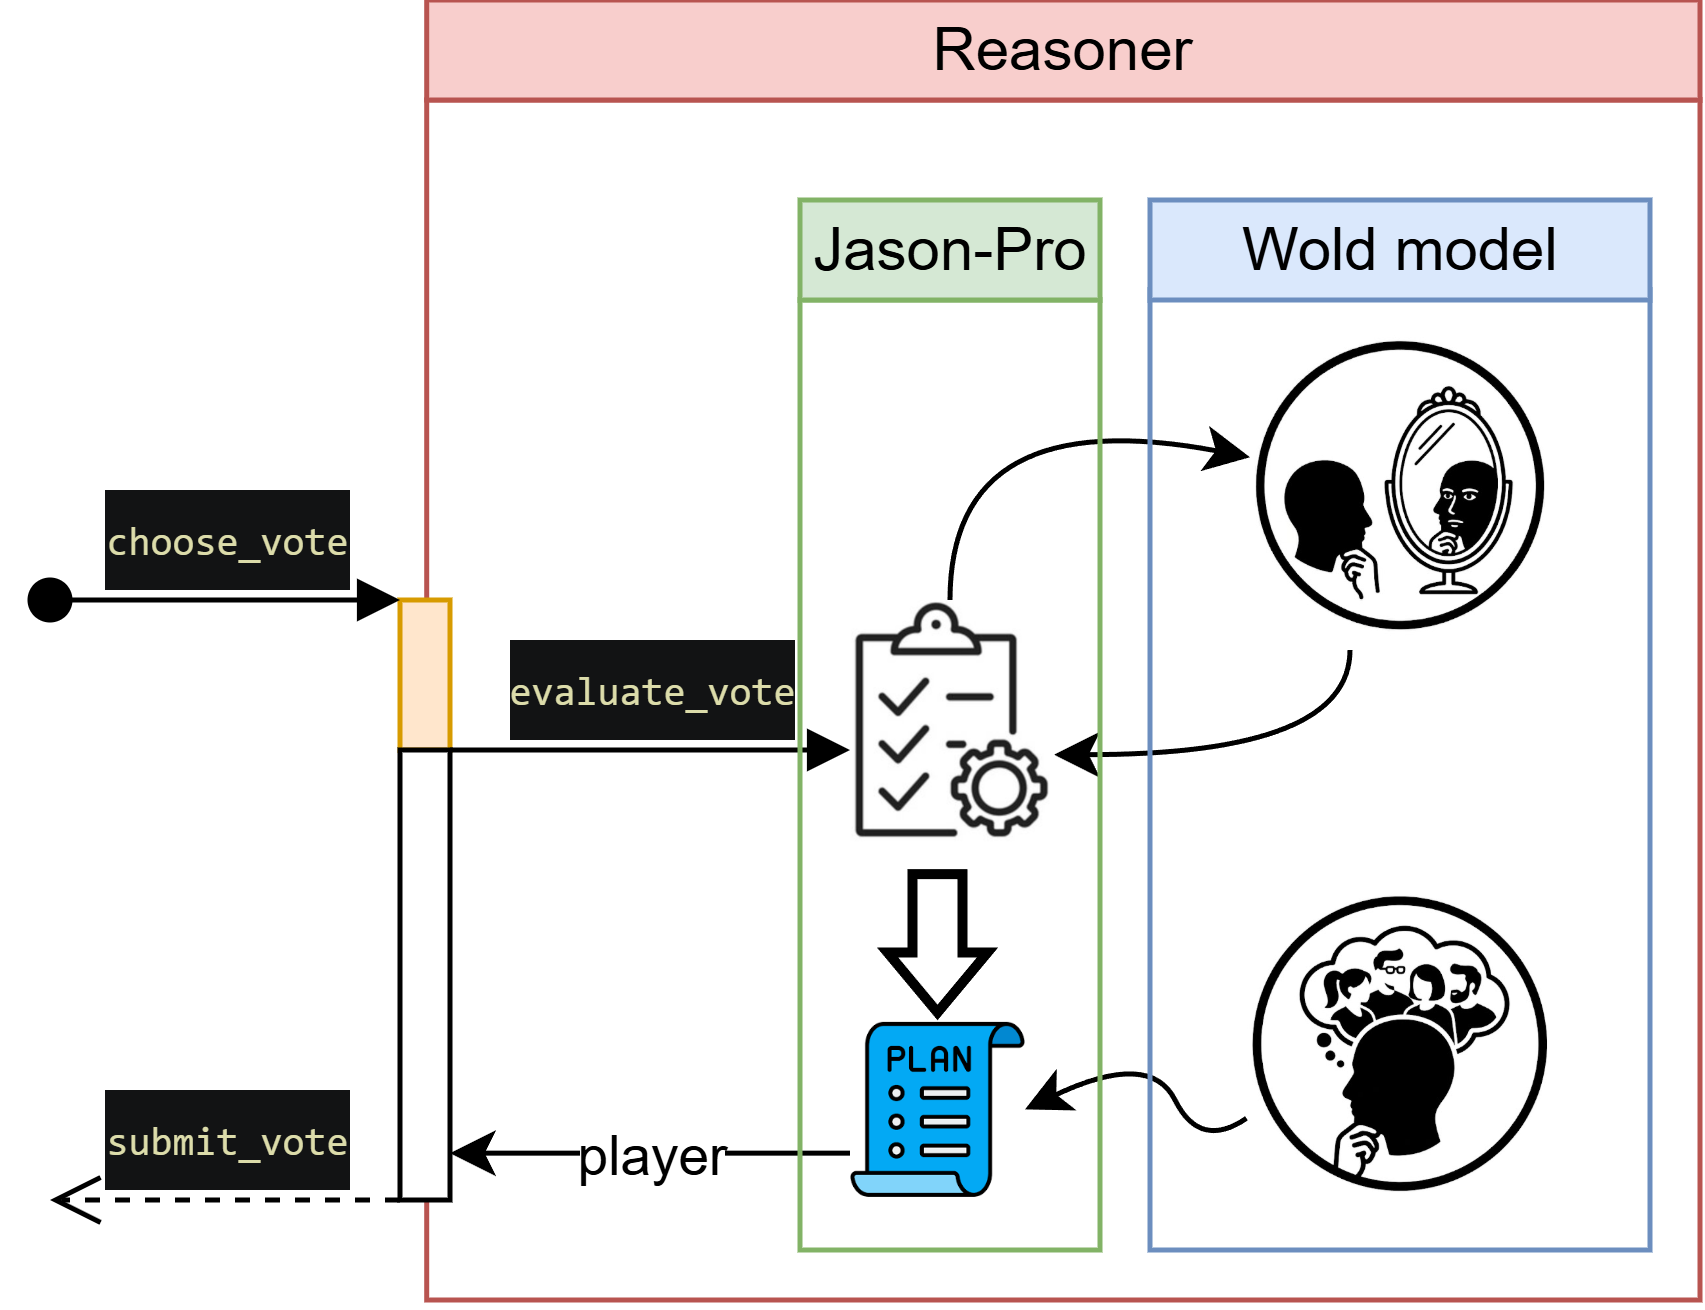
\includegraphics[width=0.6\textwidth]{images/symbolic_reasoner/read_on_symbolic_reasoner.png}
    \caption{Execution pipeline for state querying: the interface delegates decision-making to the reasoner, which selects a plan based on temper and queries the belief matrix to do its choice. Before the selection of the most suitable plan, a random ``artifical delay`` is implemented to ensure that belief base is fully up-to-date.}
    \label{fig:symbolic_reasoner_read}
\end{figure}
The reasoner also can query its belief base to make active decisions (Figure \ref{fig:symbolic_reasoner_read}). 

Because this process uses the same plan's selection pipeline of state updates, decision-making by design can trigger temper shifts, again by using \texttt{effect(...)}.
\begin{verbatim}
    @voting_panicked[ temper([stress(0.8)[mood], paranoia(0.7)]), 
                     effects([stress(-0.5)[mood]]) ]
    +!evaluate_vote(Target) 
        :   other_players(Others) 
        <-  ?select_by_trait(max, suspicion, Others, Target).
\end{verbatim}


To safely extract targets from the raw belief base, the reasoner utilizes the query mechanics defined in \texttt{reasoners/symbolic/utils.asl} (Listing \ref{lst:query_utils}): first is ensured the lazy initialization of the Attr on all the Candidates, then based on that mapping only, a Target is chosen.

\begin{lstlisting}[frame=single, language=Prolog, caption={Implementation of the querying utilities. The wrapper enforces lazy initialization before safely aggregating and extracting the optimal candidate.}, label={lst:query_utils}]
//strategies:  min,max,random
pick_by_strategy(min, [val(_, T) | _], T).
pick_by_strategy(max, Sorted, T) :- Sorted \== [] 
    & .reverse(Sorted, [val(_, T) | _]).
pick_by_strategy(random, Candidates, Target) :- 
    random_target(Candidates, Target).
//fallback for empty list: return self 
pick_by_strategy(_, [], T) :- .my_name(T).

+?select_by_trait(Op, Attr, Candidates, Target)
    <-  //lazy initialization
        for ( .member(P, Candidates) ) 
            { ?trait(P, Attr, _); };        
        .findall(val(V, P), 
            (.member(P, Candidates) & trait(P, Attr, V)),
            List);
        .sort(List, Sorted);
        ?pick_by_strategy(Op, Sorted, Target).
\end{lstlisting}



\section{The User Interface (UI)}
\label{sec:ui}

While the Multi-Agent System can run autonomously, actual gameplay requires a ``Human-in-the-Loop'' (HITL) interface. The GUI was built natively in Java for seamless integration with Jason.
Since this front-end was outside the scope of the project, only the high-level design was hand-crafted, while \textbf{the code was primarily vibe-coded using Gemini Pro 3.1 and Claude Opus 4.6}.

\subsection{``Human'' Reasoner}
\label{subsec:human-player}

Implementing the interface to allow for human interaction bypasses the cognitive pipeline defined previously. Unlike autonomous agents, the human player does not utilize the \texttt{vesna.ProAgent} engine nor the epistemic trait matrix, relying entirely on their own heuristics.

For this reason, the Jason file (\texttt{reasoners/human/interface.asl}) simply defines a synchronization layer between the asynchronous GUI and the Jason execution cycle.

When the Narrator requests an action, the agent updates the GUI and then suspends its active intention, remaining idle until the user interacts with the interface. As demonstrated in Listing \ref{lst:human_vote_hook}, this physical interaction triggers a Java callback that injects the awaited belief directly into the agent's belief base. This new belief satisfies the blocking condition, restoring the plan and submitting the human's choice back to the Narrator.

\begin{lstlisting}[frame=single, language=Prolog, caption={Example of a UI execution hook. Once notified the start of the hunting phase the ui is updated to allow the voting; the Agent's intention to choose a target halts using \texttt{.wait} and resumes immediately once the human interaction injects the \texttt{user\_input} belief.}, label={lst:human_vote_hook}]
+!manage_phase(peasant_vote, Phase_title, Msg) 
    <-  ui.actions.start_vote(Phase_title, Msg, "vote");

+!choose_vote
    <-  .wait(user_input(RawTarget)); 
        -user_input(RawTarget); 
        .term2string(Target, RawTarget);
        !submit_vote(Target).
\end{lstlisting}

\subsection{Dashboard Layout and Visualizer}
\label{subsec:ui-layout}

To provide real-time transparency into the simulation, each player can instantiate\footnote{Each player can activate its own interface by adding \texttt{setting(spectator\_mode(true))} to their belief base. Furthermore, defining it inside the Narrator's belief base instantiates a windows for each player in the game} a dedicated graphical dashboard that acts as an explicit visualizer of its current state. As shown in Figure \ref{fig:ui_dashboard}, the interface is structurally divided into three panels:

\begin{figure}[H]
    \centering
    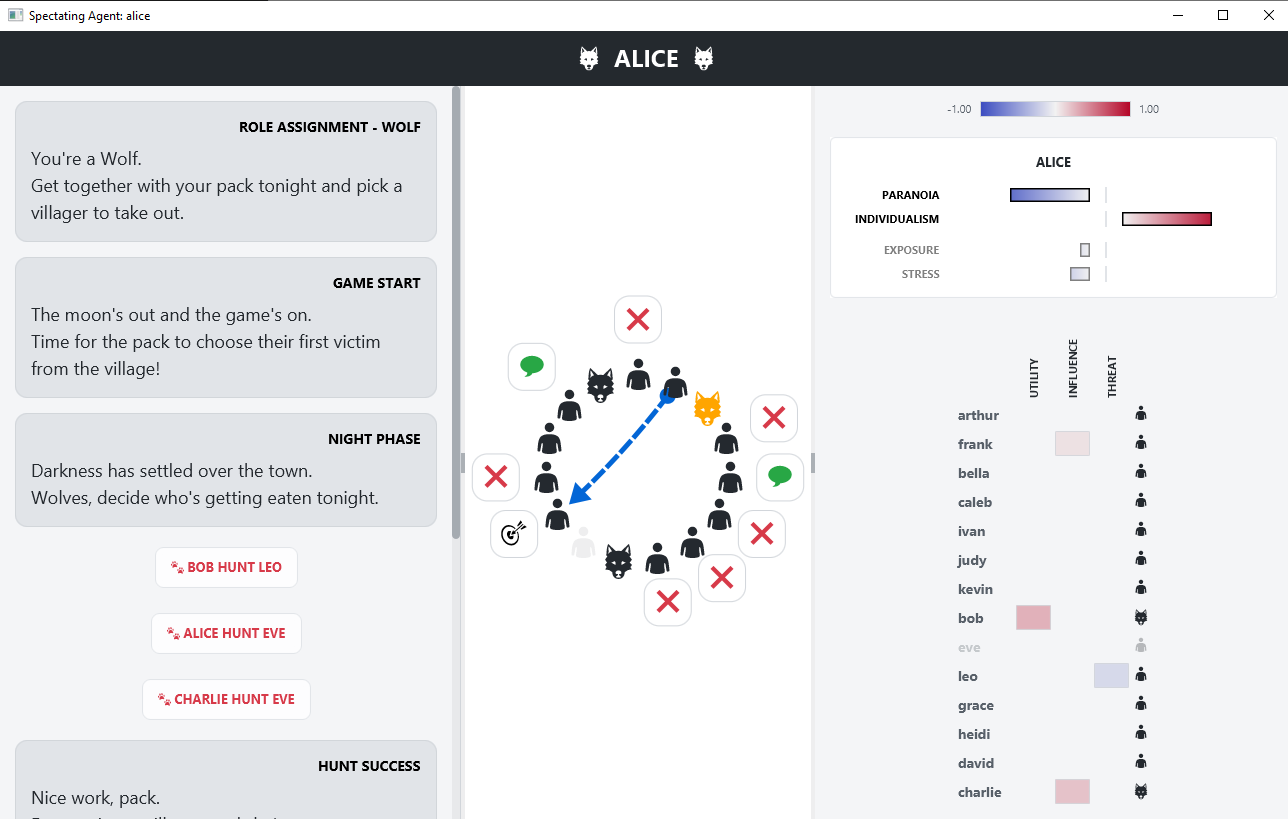
\includegraphics[width=1\textwidth]{images/UI.PNG}
    \caption{The real-time player dashboard. The left panel tracks the event log, the center maps directed actions, and the right exposes the agent's internal cognitive models. If interactions are needed, a fourth panel, centered on the bottom, appears and dictates what to do.}
    \label{fig:ui_dashboard}
\end{figure}

\begin{itemize}
    \item \textbf{Left Panel (Event Log):} Displays the chronological event sequence, encompassing Narrator announcements, broadcast messages from other agents, and a categorical recap of phase actions (e.g., hunting or voting summaries).
    \item \textbf{Center Panel (Spatial Graph):} Shows a circular node representation of all active players. It visually maps directed actions using arrows, explicitly tracing execution targets and the performatives of speech acts between agents.
    \item \textbf{Right Panel (Cognitive State):} Visualizes the agent's internal \textbf{world model}, tracking both its affective \texttt{temper} (mood and personality parameters) and its epistemic belief matrix regarding other players in real time\footnote{By design, this panel is completely disabled if the dashboard is assigned to a human player, as they do not need the engine's internal trait modeling or affective heuristics.}.
\end{itemize}

For human-driven players, the dashboard is mandatory, and transitions from a passive visualizer to an active input mechanism. When the agent's execution hook pauses to await a decision (as detailed in Section \ref{subsec:human-player}), the UI explicitly prompts the human operator for action.

\section{LLM Integration}
\label{sec:llm}

Although the core multi-agent logic is fully functional and playable, this baseline simulation lacks narrative immersion. The Narrator's messages are hard-coded, hence zero variability across different rounds;  furthermore, the players' speech are only reduced to their speech acts, without a textual human-readable part.


\begin{figure}[H]
    \centering
    % Left side: Without LLM
    \begin{subfigure}[b]{0.48\textwidth}
        \centering
        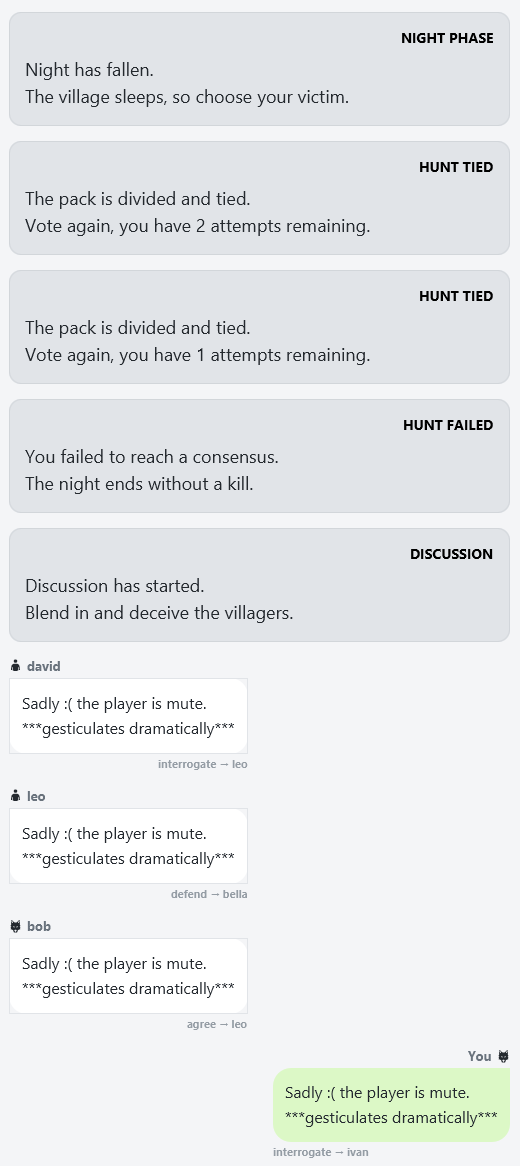
\includegraphics[width=\textwidth]{images/chat_no_llm.PNG} % Update with your actual filename
        \caption{Without LLM: Rigid, prefab messages lacking immersion.}
        \label{fig:chat_no_llm}
    \end{subfigure}
    \hfill
    % Right side: With LLM
    \begin{subfigure}[b]{0.48\textwidth}
        \centering
        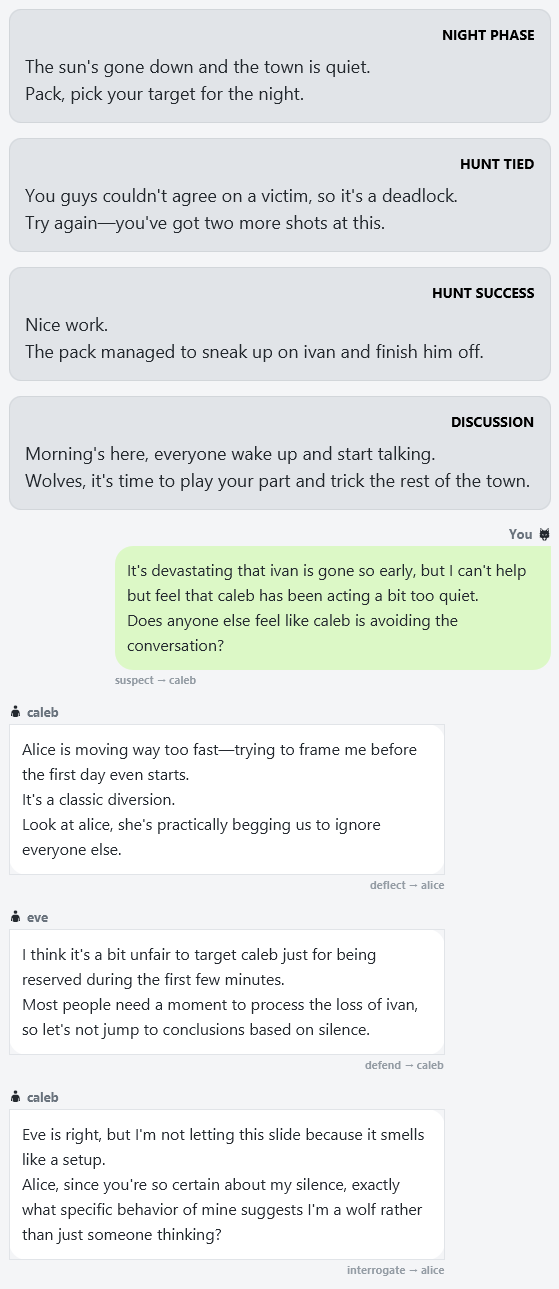
\includegraphics[width=\textwidth]{images/chat_llm.PNG} % Update with your actual filename
        \caption{With LLM: Organic, immersive dialogue for both players and the Narrator.}
        \label{fig:chat_with_llm}
    \end{subfigure}
    
    \caption{Comparison of the game's chat interface. The integration of the LLM transforms the interaction from abstract speech acts (left) into a narrative roleplay experience (right).}
    \label{fig:llm_chat_comparison}
\end{figure}

To bridge the gap between abstract symbolic reasoning and human-readable roleplay, the architecture integrates a \textbf{Large Language Model} to generate  immersive dialogue. To avoid API costs, the proposed bridge connects strictly to local models, hosted using \textbf{Ollama}, interfaced through a custom Java wrapper (\texttt{src/llm/OllamaAPI}).

\paragraph{Verifying Connectivity and Model Warm-up}
Before any text generation occurs, the system must validate the local LLM environment. During the Narrator's boot sequence, the agent executes a custom internal action (\texttt{llm.ping\_llm}) to establish a handshake with the Ollama server. This ping serves three critical architectural purposes:

\begin{enumerate}
    \item \textbf{GPU Warm-up:} By default, Ollama loads models into memory only when queried, which introduces severe "cold-start" latency on the first request. The ping explicitly passes the \texttt{"keep\_alive":-1} parameter in its JSON payload, forcing the Ollama server to load the requested model directly into VRAM and hold it there indefinitely, to ensure faster response time.
    
    \item \textbf{Model Validation:} It verifies that the Ollama service is actively running on the local port and that the specific model requested by the simulation settings is actually installed on the machine.
    
    \item \textbf{Error Handling:} If the connection is refused or the model is missing, the Java API catches the exception and returns a specific error string to the Jason environment. This allows the multi-agent system to safely abort the LLM initialization and disable any module that requires it. By catching this during the warm-up phase, the simulation can seamlessly fall back to the "bland" symbolic logging mode without crashing mid-game.
    
\end{enumerate}


\subsection{Prompting the LLM}
\label{subsec:llm_communication}

The communication layer that bridges the Jason logic and the LLM is handled by two dedicated Java classes: \texttt{LLMUtils} and \texttt{OllamaAPI}. In this architecture, the logical content of the prompt is determined entirely within Jason, while the Java layer simply glues together and sanitizes the strings. The assembled prompt is then sent to the LLM, and finally, the result is post-processed to ensure a safe output.

\begin{figure}[H]
    \centering
    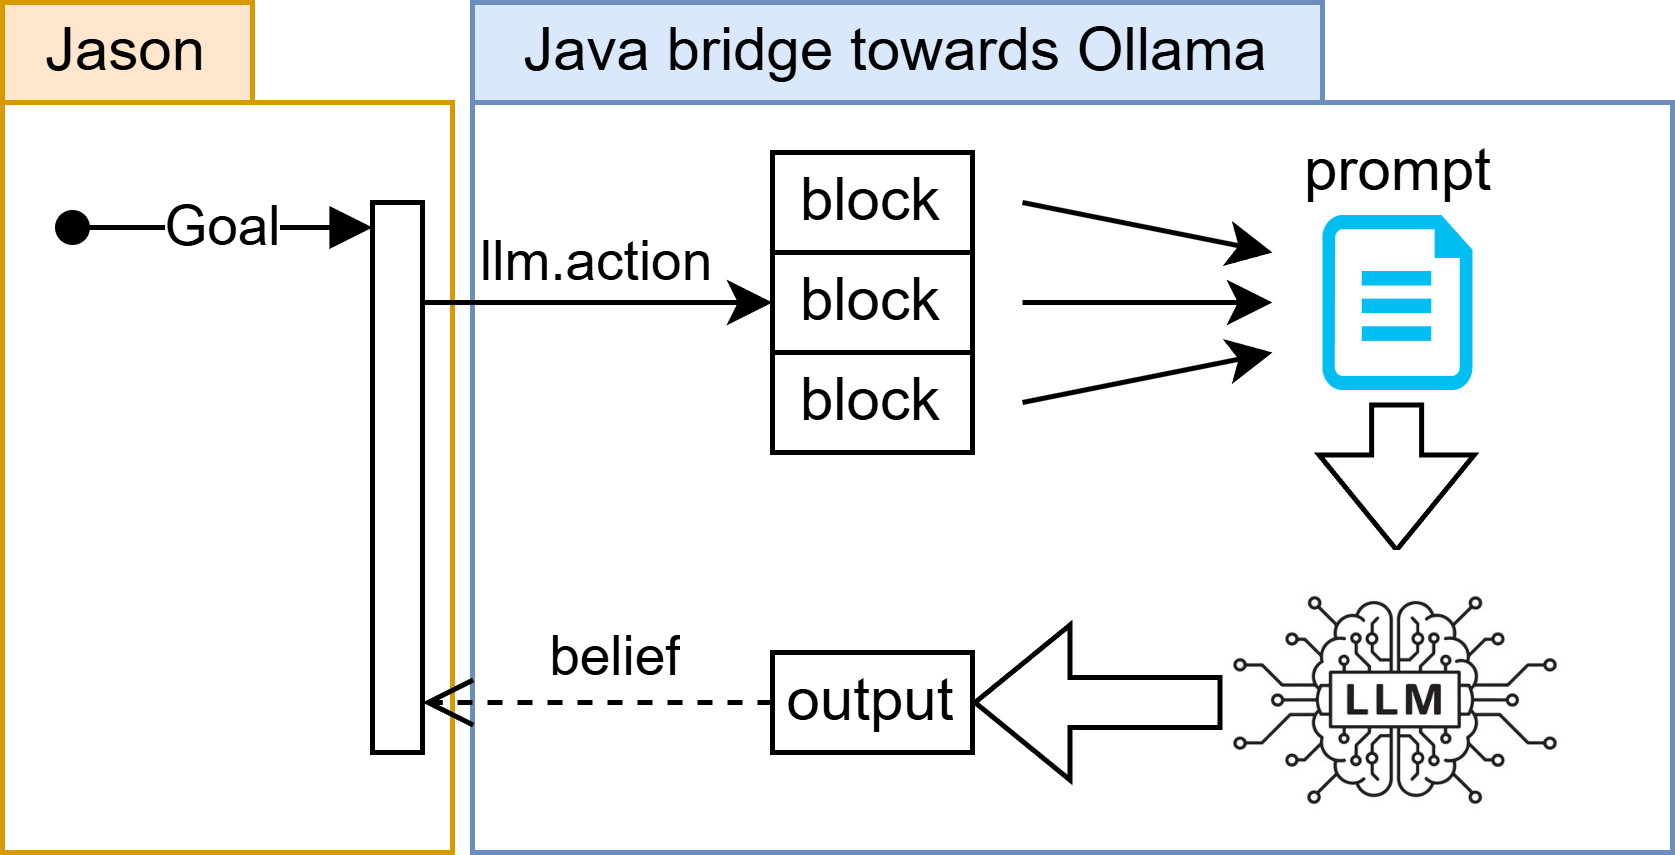
\includegraphics[width=0.8\textwidth]{images/ollama_bridge.png}
    \caption{Interaction between the Jason Engine and the Ollama API. A custom Java action is called by passing ``building blocks'' as input; they are merged into a prompt given to the LLM, and the output is directly injected as a belief into the agent.}
    \label{fig:ollama_bridge}
\end{figure}

To streamline query management, the system utilizes \texttt{LLMUtils.PromptBuilder}, which constructs prompts by appending modular text blocks to improve code reusability.

Once the full prompt is assembled, it is routed to the \texttt{OllamaAPI}. This class wraps the prompt into a JSON payload and issues an HTTP POST request directly to the local model. Once the response is received, the class extracts the generated text and, if configured, saves the full interaction payload to a local directory for later debugging and analysis. The raw output is then routed back through \texttt{LLMUtils}, which sanitizes the text to prevent parsing failures. The sanitized string is wrapped into a Jason \texttt{Literal} and asynchronously injected into the agent's belief base, triggering a \texttt{wakeUpSense()} call to immediately resume the agent's execution cycle.

\paragraph{Stateless Execution Bottleneck}
A critical observation is that the LLM is treated as a purely stateless function. The \texttt{OllamaAPI} does not maintain hidden states or conversation memory between calls\footnote{This implementative choice is defined by the way the LLM reasoner was designed: each action is completely independent, and the only state kept between them must be explicitly defined as a Jason belief. Furthermore, the Ollama API must be completely agnostic to the game size; hence, keeping a conversation open for each player could result in a VRAM shortage.}. Consequently, every request is atomically independent, requiring the prompt to redefine the complete context from scratch. While the model remains pre-loaded in the GPU, handling concurrent queries with massive contextual payloads renders the system highly susceptible to computational bottlenecks (as highlighted in Section \ref{sec:results}).


\paragraph{Bridging Symbolic Logic and Natural Language}
A substantial portion of the development effort was dedicated to the non-trivial challenge of designing an explicit, deterministic encoding that translates the agents' hidden symbolic states (i.e the Agent's beliefs) into flexible natural language prompts. To ensure contextual accuracy and narrative immersion, the language model required absolute integrity regarding the current game state. 

However, strict hardware limitations constrained the architecture to rely on smaller LLMs: these compact models proved highly susceptible to \textbf{contextual drift and catastrophic hallucination} when exposed to specific token or overloaded context windows\footnote{A example of this contextual drift that can be appreciated on the tested model is provided in Section \ref{sec:results}.}. Consequently, crafting modular prompts  rigid enough to prevent hallucination, yet flexible enough to cover  each possible state of the game, required extensive (both temporal and testing-wise) iterative trial-and-error. The Prompt defined in the next parts are hence the results of this long process.

\subsection{Enhancing Narration}
\label{subsec:llm-narration}
As detailed in Section \ref{sec:narrator}, the transition along the edges of the game's state machine is strictly managed by the Narrator. In the baseline implementation, state transitions are broadcastes using hard-coded messages, stored in \\
\texttt{narrator/core/game\_narration.asl}. These default templates are parametric and defined by a unique identifier, a phase title, a specific conversational intent (the core speech act it must convey), and a default base message.

\begin{lstlisting}[frame=single, language=Prolog, caption={Example of a parametric narration template. The rule dynamically binds variables to generate the title, intent, and default message.}, label={lst:narrator_msg_template}]
narrator_message(exec_result,[villagers, villager, Victim], PhaseTitle, PhaseIntent, Message) :-
    PhaseTitle = "Execution Result - Failure" &
    .concat("Announce to the village that the executed player ", Victim, " was an innocent villager.", PhaseIntent) &
    .concat("A tragic mistake. The town executed ", Victim, ", an innocent villager.", Message).
\end{lstlisting}

If the LLM module is enabled, the agent dynamically aggregates its predefined speaking style, retrieves the most recent phase logs, and translates them into a human-readable context block. 

\begin{lstlisting}[frame=single, language=Prolog, caption={Simplified dispatch logic for the Narrator. It retrieves the required context and asynchronously queries the Java API, safely falling back to the base message if the LLM generation fails.}, label={lst:narrator_dispatch}]
?msg(_, BaseMessage, PhaseTitle, PhaseIntent, _);
if (setting(llm_narrator(true))) {
    ?narrator_style(StyleDesc);
    ?setting(narrator_chunk_log_size(NarratorChunkLogSize));
    ?get_log_chunk(any, TargetList, NarratorChunkLogSize, LogChunk);
    ?translate_log(LogChunk, LogChunkTranslated);
    
    llm.narrator_message(PhaseIntent, BaseMessage, StyleDesc, LogChunkTranslated);
    .wait(narrator_result(FinalMessageString));
    -narrator_result(_);
} else {
    FinalMessageString = BaseMessage;
};
\end{lstlisting}

The \texttt{StyleDesc} variable is populated by a hard-coded belief that dictates the Narrator's persona, ensuring a consistent ``tabletop game master'' tone throughout the Game.

\begin{lstlisting}[frame=single, language=Prolog, caption={The Narrator's style definition explicitly outlines the tone, vocabulary, and prohibitions.}, label={lst:narrator_style}]
narrator_style(Desc) :- 
    .concat("- TONE: Conversational, engaging, slightly dramatic but clear.\n",
            "- VOCABULARY: Natural tabletop language (e.g., 'You guys', 'The village'). Use contractions.\n",
            "- FOCUS: Setting the mood while delivering phase mechanics.\n",
            "- PROHIBITION: DO NOT sound like a robotic terminal. DO NOT use overly formal words.", 
            Desc).
\end{lstlisting}

Finally, the extracted data blocks ( the intent, the base message, the style description, and the translated history log) are passed to the custom Java internal action \texttt{llm.narrator\_message}. This wrapper utilizes the \texttt{PromptBuilder} utility to construct the structured prompt, appending each piece of data into modular text blocks.

\newpage
\begin{lstlisting}[frame=single, basicstyle=\scriptsize\ttfamily, breaklines=true, caption={The fully assembled prompt sent to the Ollama API. Each block is vital to prevent the LLM from hallucinating or copying the messages sent before.}, label={lst:narrator_prompt}]
### WORLD SETTING
You are participating in a multi-agent simulation of the game Werewolf/Mafia.

### YOUR IDENTITY
ROLE: TABLETOP GAME MASTER / NARRATOR

### STYLE OF SPEECH
- TONE: Conversational, engaging, slightly dramatic but clear.
- VOCABULARY: Natural tabletop language. Use contractions.
- FOCUS: Setting the mood while delivering phase mechanics.
- PROHIBITION: DO NOT sound like a robotic terminal. DO NOT use overly formal words.

### REFERENCE MESSAGE
A tragic mistake. The town executed heidi, an innocent villager

### YOUR CURRENT GOAL
INTENT TO CONVEY: Announce to the village that the executed player heidi was an innocent villager.

### RECENT DIALOGUE HISTORY 
- [NARRATOR]: Tough break, guys. You just kicked out Frank, and he was totally innocent.
- [NARRATOR]: Lights out, everybody. Try to stay safe while the pack begins their hunt.
- [NARRATOR]: Rise and shine, folks. It's a grim start to the day because Ivan was taken out...
- [NARRATOR]: Alright, floor's open. Start digging into each other and root out the monsters!
- [NARRATOR]: Discussion's closed. It's time to lock in your choices!

### RESPONSE CONSTRAINTS (MANDATORY)
1. STRICT LIMIT: Output 1 to 3 sentences maximum.
2. NO PARROTING: Use the REFERENCE MESSAGE strictly for factual pacing. Write entirely new dialogue.
3. VOCABULARY VARIATION: You are strictly forbidden from using opening greetings present in the HISTORY.
4. NO REPETITION: Do not reuse any specific wording from the HISTORY nor the REFERENCE MESSAGE.
5. ASSUMED CONTEXT: Focus strictly on the INTENT TO CONVEY. Assume players possess full knowledge of past events.
6. FORMAT: Output ONLY the raw response string. No meta-commentary, no JSON, no markdown.
7. ONE-LINE: The output must be a single line of text, without line breaks or paragraphs.

GENERATE RESPONSE NOW:
\end{lstlisting}


\paragraph{Empirical Prompt Tuning}
During development, empirical testing revealed that each discrete block within the prompt structure is critical for stabilizing the output of the quantized LLM. Specifically:
\begin{itemize}
    \item \textbf{\texttt{\#\#\# STYLE OF SPEECH}:} Mitigates the model's inherent verbosity and enforces strict role-playing boundaries, preventing out-of-character responses.
    \item \textbf{\texttt{\#\#\# REFERENCE MESSAGE}:} Acts as a \textbf{One-Shot} learning anchor. Testing demonstrated that relying solely on the \texttt{INTENT} causes massive hallucination; giving a structural baseline grounds the text generation.
    \item \textbf{\texttt{\#\#\# RECENT DIALOGUE HISTORY}:} Serves as a negative constraint to prevent repetitive phrasing. However, testing also revealed a strict trade-off: passing an excessively large log chunk overwhelms the small model's attention span, causing it to parrot previous lines rather than generate novel text.
    \item \textbf{\texttt{\#\#\# RESPONSE CONSTRAINTS}:} Enforces rigid syntactic formatting, ensuring the raw output string integrates organically into the Java UI chat panel without breaking the display logic.
\end{itemize}

\subsection{LLM Reasoner (Ollama)}
\label{subsec:llm-reasoner}
Building on the logic used for the Narrator's message enhancement, it is possible to define the final type of reasoner: the LLM-powered reasoner. To minimize modifications to the Symbolic Reasoner's architecture, is kept the same blueprint for its internal state, defined by the agent's self-awareness beliefs and Trait Matrix (and also other internal beliefs). However, in this context, we require a \textbf{textual encoding} process to convert these symbolic values into \textbf{blocks} that can be used to construct the prompt.

\subsubsection{Textual Encoding of the Agent State}
\label{subsubsec:llm-reasoner-encoding}
The files responsible for this symbolic-to-text translation are modularly organized within the \texttt{shared/llm\_context/} directory. Rather than relying on a single monolithic parser, each script is dedicated to decoding a specific dimension of the agent's knowledge base, such as conversation history, active traits, or psychological temperament. Each files operates indipendenlty and is loaded at  runtime (if needed), during the player's initialization.

\paragraph{\textbf{\texttt{log\_2\_context.asl}}} 
This module handles the integral log stored by the narrator in its belief base. It defines the core rule \texttt{translate\_log(LogChunk, TextualEncoding)}, that given a raw list of the Narrator's log events, encodes it in a list of text lines. Because the log is structured as a sequence of nested Prolog literals (e.g., \texttt{action(speech(...))}), the rule recursively iterates through the list, pattern-matching specific game events and mapping them to predefined string templates. Finally, it concatenates these translated entries into a single, chronologically formatted text block. 

\begin{verbatim}
log_to_text(action(speech(Src, Msg, Int)), S) :-
    .concat("- [", Src, " -> ", IntStr, "]: ", Msg, S).

log_to_text(action(victim(hunt, Vic, R)), S) :-
    .concat("    - ", Vic, ", a ", R, 
            " was killed by the hunt of the wolves.", S).

log_to_text(action(victim(vote, Vic, R)), S) :-
    .concat("    - ", Vic, ", a ", R, 
            " was eliminated by the village.", S). 

log_to_text(action(hunt_vote(Src, Tgt)), S) :-
    .concat("    - ", Src, " hunted ", Tgt, S).

log_to_text(action(vote(Src, Tgt)), S) :-
    .concat("    - ", Src, " voted for ", Tgt, S).
\end{verbatim}

\paragraph{\textbf{\texttt{performatives\_2\_context.asl}}} 
It defines a set of rules to translate the (abstract) speech acts into explicit natural language instructions. It maps each symbolic performative to a precise behavioral instruction detailing how the LLM should construct its message. The rules are parametric in the Player's Name, to define a explicit guide for the LLM. The defined mappings are as follows:

\begin{itemize}
    \item \textbf{\texttt{accuse(\{PLAYER\})}:} 
        ``Aggressively accuse \{PLAYER\} of being a wolf and push the village to execute them.''
    \item \textbf{\texttt{defend(\{PLAYER\})}:} 
        ``Defend \{PLAYER\} against current suspicions and argue for their innocence.''
    \item \textbf{\texttt{suspect(\{PLAYER\})}:} 
        ``Express heavy suspicion towards \{PLAYER\} without fully committing to an accusation.''
    \item \textbf{\texttt{agree(\{PLAYER\})}:} 
        ``Strongly agree with the recent statements or tactical direction of \{PLAYER\}.''
    \item \textbf{\texttt{interrogate(\{PLAYER\})}:} 
        ``Ask a direct, pressuring question to \{PLAYER\} to force them into a mistake or contradiction.'
    \item \textbf{\texttt{deflect(\{PLAYER\})}:} 
        ``Deflect any current suspicion away and firmly redirect the village's attention onto \{PLAYER\}.''
\end{itemize}


\paragraph{\textbf{\texttt{traits\_2\_context.asl}}} 
This module translates the agent's epistemic belief matrix into a structured psychological context block. It first formally describes the active traits in natural language, dynamically adapting the definitions based on the agent's assigned role:

\begin{itemize}
    \item \textbf{\texttt{suspicion}} (Villagers only): ``A low level means you believe they are innocent and trustworthy, while a bigger value means you strongly suspect they are a wolf.''
    \item \textbf{\texttt{threat}} (Wolves only): ``A low level means they are ignoring you or pose no danger, while a bigger value means they are actively attacking you or your pack.''
    \item \textbf{\texttt{utility}}: ``A low level means they are an obstacle or useless to your strategy, while a bigger value means they are actively helpful to your goals.''
    \item \textbf{\texttt{influence}}: ``A low level means they are losing credibility or looking foolish, while a bigger value means they are highly persuasive and leading the game.''
\end{itemize}

Second, it aggregates the current numerical trait values for every other player into a formatted list. A critical implementation detail is the explicit randomization of the player array (using \texttt{.shuffle}) prior to converting the players' profiles into text. This step is necessary to mitigate the LLM's inherent \textbf{positional bias} toward specific players\footnote{This highlights a key observation discussed in Section \ref{sec:results}: this mitigation strategy alone is insufficient to shift the LLM's inherently biased decision-making process toward a completely agnostic (equiprobable) distribution.}.

Furthermore, since the traits are lazily evaluated, some players might not have any defined traits at a given moment. To account for this missing data, an explicit string is appended on top of the prompt instructing the LLM on how to interpret the absence of values.


\begin{lstlisting}[frame=single, basicstyle=\footnotesize\ttfamily, breaklines=true, caption={Example of the generated trait context block for a wolf agent. Not each trait of the players is defined, and only the ``alive'' ones are listed.}, label={lst:traits_context}]
    CURRENT EPISTEMIC OPINIONS TOWARDS OTHER PLAYERS:
    NOTE: Any traits not listed is 0.0 (Unbiased/Neutral opinion)
    
    ivan(influence: 0.41, utility: 0.38, suspicion: 0.11)
    judy(utility: 0.11, influence: 0.05)
    arthur(influence: 0.41)
    bob(suspicion: 0.53, influence: 0.13)
    grace(suspicion: -0.15, utility: 0.12, influence: 0.03)
    kevin(utility: 0.51)
    eve(suspicion: 1, influence: 0.53)
\end{lstlisting}


\paragraph{\textbf{\texttt{temper\_2\_context.asl}}} 
Is the module accountable for the translation of the agent's self-aware metrics. It is divided into two distinct parts. The first part defines the player's constant personality traits, including their role, name, and static moods. To convert continuous numerical values into human-readable text, each mood's domain is discretized into five bins. Each bin maps directly to an explicit behavioral archetype.

\begin{lstlisting}[frame=single, basicstyle=\footnotesize\ttfamily, breaklines=true, caption={Discretization of the continuous \texttt{paranoia} trait into five distinct behavioral bins. The \texttt{ProAgent} engine evaluates the numerical value to select the appropriate natural language description.}, label={lst:paranoia_bins}]
@paranoia_very_high[ temper([paranoia(1.0)]) ]
+!compile_paranoia_rule(Rule) 
    <-  .concat("- CONSPIRACIST: You are a true conspiracist. You trust absolutely no one (except your own packmates, if any), assume every statement is a trap, and see conspiracies everywhere.", Rule).

@paranoia_high[ temper([paranoia(0.5)]) ]
+!compile_paranoia_rule(Rule) 
    <-  .concat("- SKEPTIC: You are a sharp skeptic. You scrutinize others' words closely looking for hidden motives and rarely take things at face value.", Rule).

@paranoia_neutral[ temper([paranoia(0.0)]) ]
+!compile_paranoia_rule(Rule) 
    <-  .concat("- REALIST: You are a grounded realist. You are cautious but willing to listen to reason and evaluate evidence fairly.", Rule).

@paranoia_low[ temper([paranoia(-0.5)]) ]
+!compile_paranoia_rule(Rule) 
    <-  .concat("- OPTIMIST: You are a hopeful optimist. You are trusting, hence you generally take people at their word and assume good intentions.", Rule).

@paranoia_very_low[ temper([paranoia(-1.0)]) ]
+!compile_paranoia_rule(Rule) 
    <-  .concat("- NAIVE: You are completely naive. You are highly trusting, implicitly believe what others tell you, and tend to ignore red flags.", Rule).
\end{lstlisting}

During player initialization, the \texttt{vesna.ProAgent} parsing logic evaluates these static temperaments, extracts the corresponding text definitions, and permanently store them within a \texttt{+player\_description(ProfileBlock)} belief to avoid redundant string concatenation during gameplay.


\begin{figure}[H]
    \centering
    
    % Top: Topology Scatter Plot
    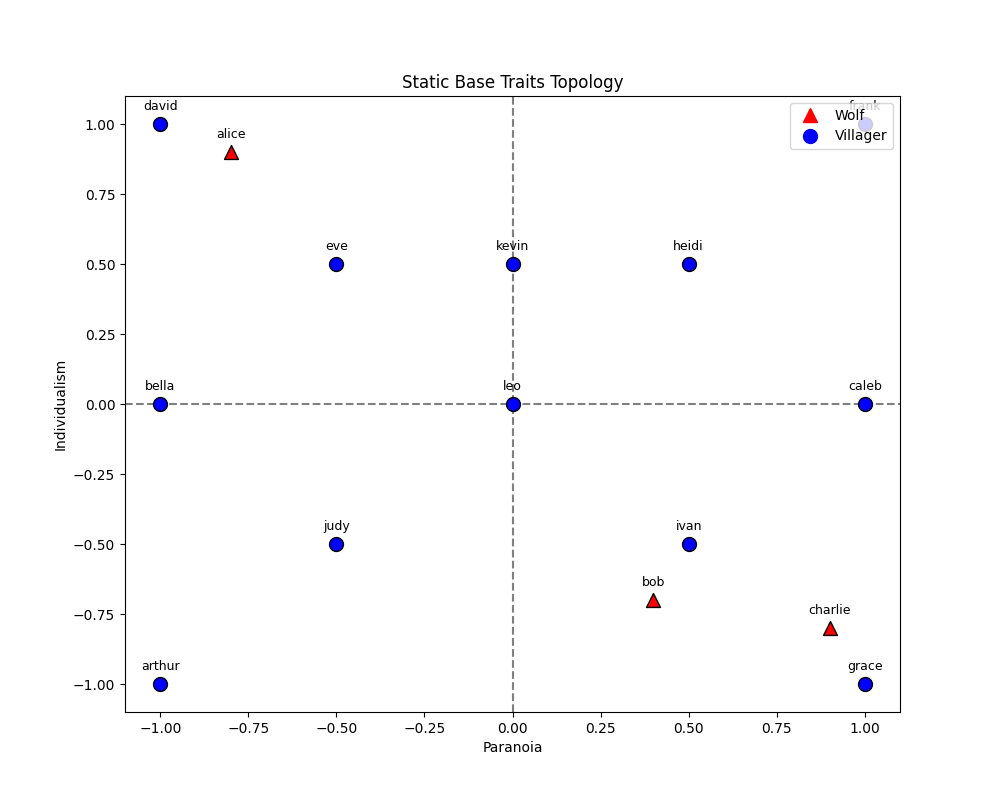
\includegraphics[width=1\textwidth]{images/personality topology.png}
    
    \vspace{1.5em} % Structural spacing between image and text blocks
    
    % Bottom: Two-column tabular for guaranteed full-height vertical divider
    \begin{tabular}{@{} p{0.47\textwidth} | p{0.47\textwidth} @{}}
        \scriptsize
        \textbf{Player Name:} alice \newline
        \textbf{Hidden Role:} wolf \newline
        \textbf{Personality Profile:}
        \begin{itemize}
            \item \textbf{NAIVE:} You are completely naive. You are highly trusting, implicitly believe what others tell you, and tend to ignore red flags.
            \item \textbf{MAVERICK:} You are a true maverick. You completely ignore the consensus of your peers, vote and act based solely on your own deductions, and refuse to follow the group.
        \end{itemize}
        &
        \scriptsize
        \textbf{Player Name:} grace \newline
        \textbf{Hidden Role:} villager \newline
        \textbf{Personality Profile:}
        \begin{itemize}
            \item \textbf{CONSPIRACIST:} You are a true conspiracist. You trust absolutely no one (except your own packmates, if any), assume every statement is a trap, and see conspiracies everywhere.
            \item \textbf{CONFORMIST:} You have a strict pack mentality. You blindly follow the choices and votes of your peers to maintain absolute unity, completely disregarding your own beliefs.
        \end{itemize}
    \end{tabular}
    
    \caption{Translation of static traits into explicit LLM prompt blocks. The exact initial spatial coordinates for agents like Alice (\texttt{paranoia}: $-0.8$, \texttt{individualism}: $0.9$) and Grace (\texttt{paranoia}: $1.0$, \texttt{individualism}: $-1.0$) define the selection of the behavioral archetypes.}
    \label{fig:traits_to_profile}
\end{figure}


\paragraph{\textbf{Speech modeling based on dynamic moods}} 
The second objective of the \texttt{temper\_2\_context.asl} module is to guarantee rhetorical guidelines during \textbf{Natural Language Generation}. The agent's speech style is structured using a hybrid prompt block: a static component that establishes broad tonal directions and explicit prohibitions (designed to inhibit the LLM's inherent stylistic biases), and a dynamic component driven by the agent's active mood variables. 

The selection logic is a the same as the previously described pipeline, utilizing the engine to extract the appropriate rhetorical goals based on real-time moods. Specifically, each injected mood string provides both a soft description of the agent's psychological state and rigid syntactic constraints that the LLM must follow to ensure immersive roleplay.

\begin{lstlisting}[frame=single, basicstyle=\footnotesize\ttfamily, breaklines=true, caption={Example of a generated speech style block. The dynamic parameters for STRESS LEVEL and SOCIAL EXPOSURE are evaluated and injected at execution time based on the agent's internal state.}, label={lst:style_of_speech}]
### STYLE OF SPEECH
- TONE: Analytical, natural. Speak like an intelligent adult in a high-stakes board game.
- STRESS LEVEL (CRITICAL): You are in a state of high panic.
  SYNTAX GUIDELINES: Speak in rushed, fragmented bursts. Use short sentences and occasional dashes (-) to show racing thoughts, but DO NOT sound cartoonish or repeat the same phrases (like 'I didn't'). Keep the vocabulary natural but urgent.
- SOCIAL EXPOSURE (NEUTRAL):You are blending into the background.
  RHETORIC GUIDELINES: Participate by asking probing questions or evaluating evidence collectively. Avoid making hard, bold declarations that would draw unnecessary attention to you.
- PROHIBITION: NO robotic academic declarations (like furthermore, therefore).
- PROHIBITION: NO cartoonish stuttering, exaggerated catchphrases, or repetitive dialogue loops. Adapt dynamically to the context.
\end{lstlisting}

Conversely, during different cognitive cycles—such as when the LLM is prompted to evaluate and update the agent's self-aware opinions regarding its own state—these continuous metrics must be formally explained rather than applied as immediate behavioral constraints. This is achieved through explicit natural language formalizations mapping the numerical domain to semantic meaning.

\begin{itemize}
    \item \textbf{\texttt{stress}:} ``A low level means you feel relieved, secure, or in control, while a bigger value means you feel panicked, pressured, or fear elimination.''
    \item \textbf{\texttt{exposure}:} ``A low level means you feel hidden, ignored, or successfully blend in, while a bigger value means you are thrust into the spotlight and suspected.''
\end{itemize}


\subsubsection{Updating the World Model}
Now that we have introduced the building blocks, we can describe how the Reasoner responds to external events. Figure \ref{fig:llm_reasoner_read} illustrates the  pipeline: symbolic beliefs are converted into textual building blocks, merged into a prompt, processed by the LLM, and then translated back into symbolic updates.

\begin{figure}[H]
    \centering
    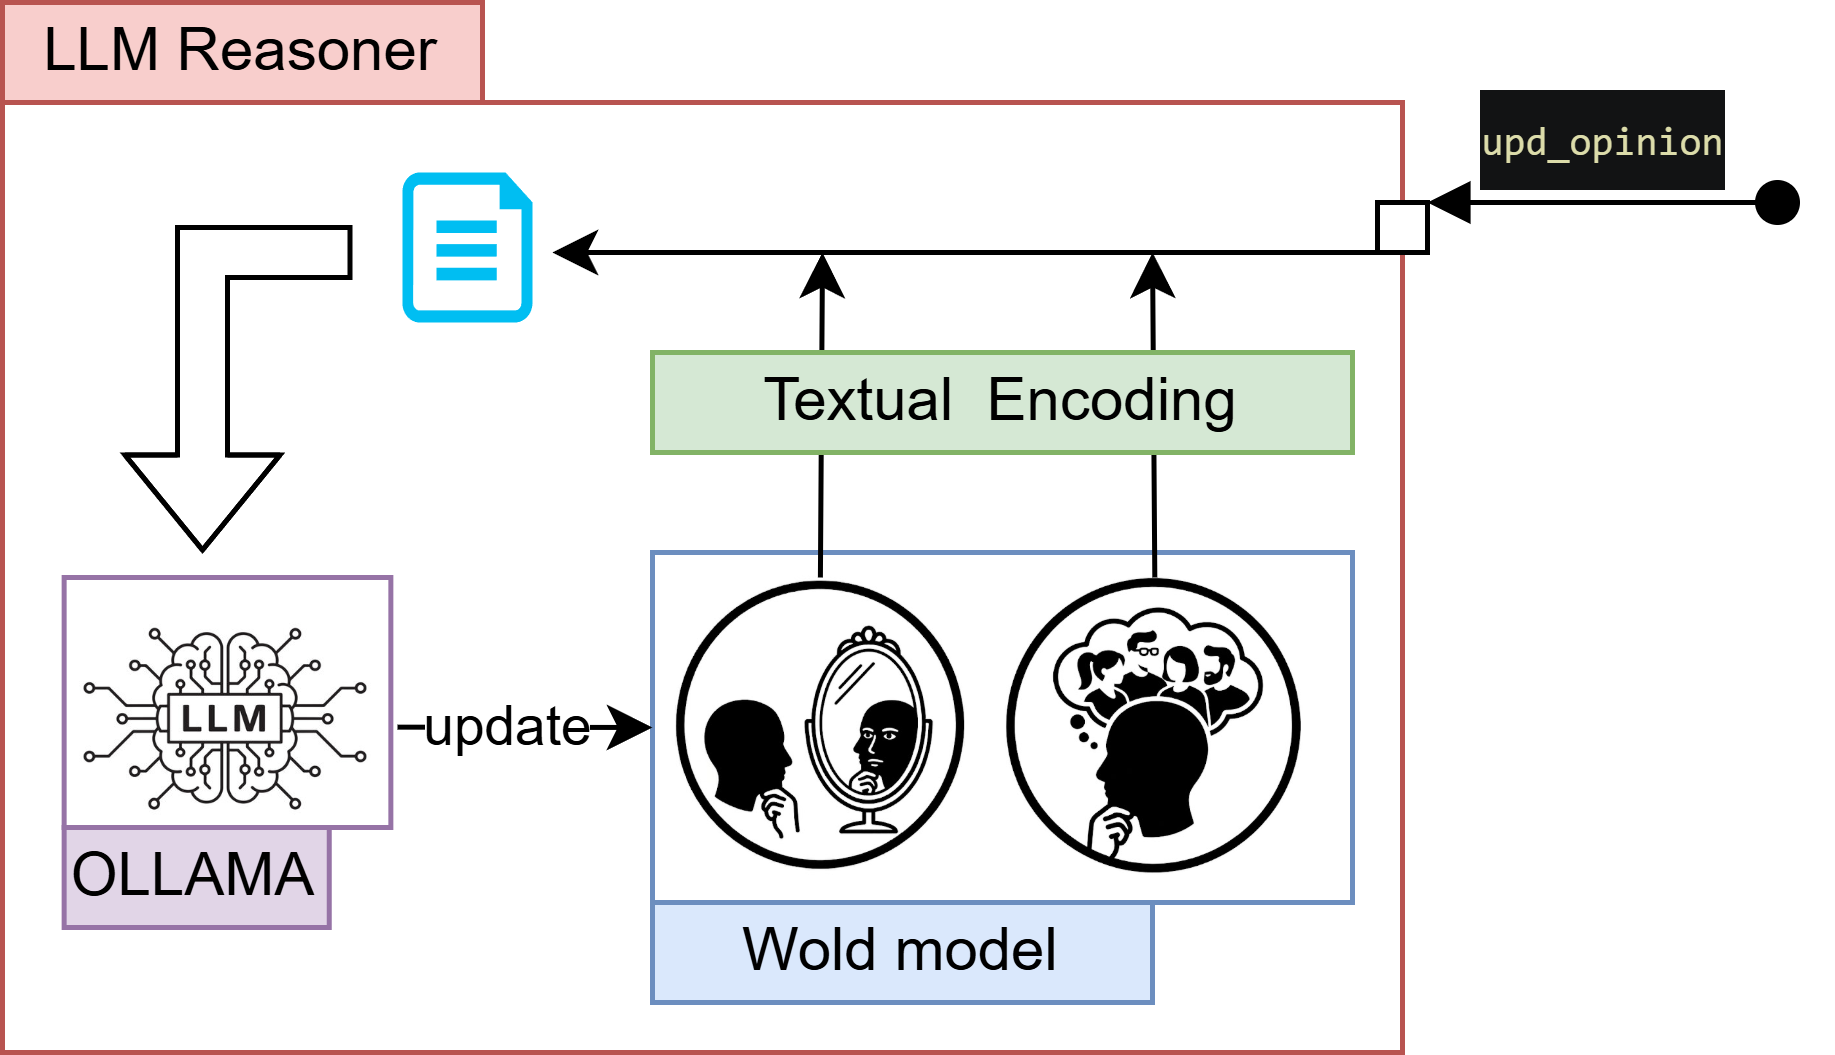
\includegraphics[width=0.8\textwidth]{images/llm_reasoner_write_on.png}
    \caption{Passive Belief's update by the Reasoner. A custom Java action is called by passing textual ``building blocks'' as input; they are merged into a prompt given to the LLM, with the output used to update the internal World Model of the Agent.}
    \label{fig:llm_reasoner_write_on}
\end{figure}

The orchestration logic in \texttt{reasoner/llm/update\_opinions.asl} counters the LLM's inherent stochasticity with robust retry mechanisms. Queries retry up to $K$ times upon failure\footnote{A common issue given the strict requirement for a perfectly formatted Jason list.}, while fallback goals (\texttt{-!invoke\_llm\_opinions}) catch exceptions to prevent system deadlocks. 

Furthermore, to avoid asynchronous race conditions when agents process multiple events concurrently, the plan dynamically generates a unique identifier (\texttt{UID}) for each LLM call (Listing \ref{lst:llm_concurrency}).

\begin{lstlisting}[frame=single, language=Prolog, caption={Implementation of concurrent execution safety. A unique identifier is generated to map the asynchronous LLM response back to the specific execution thread.}, label={lst:llm_concurrency}]
.random(RandNum);
.concat("UID_", RandNum, UID);

//call the async action, giving the blocks
llm.update_opinions(UID, IdentityContext, TraitsOpinionsString, LLMFriendlyLog, WolfPackStr, ActionStr, TraitsListStr, MoodsListStr);
        
//await the specific beliefdefined by UID
.wait(opinions_result(UID, UpdatesString));

//remove, since no more useful
-opinions_result(UID, _);
\end{lstlisting}

This ensures that the \texttt{.wait()} operator only resumes when the custom Java action injects the target belief signature matching the specific thread's \texttt{UID}, preventing the multi-agent system from deadlocking or mixing up responses.

\vspace{1em}

\begin{lstlisting}[frame=single, basicstyle=\scriptsize\ttfamily, breaklines=true, caption={Example of a complete prompt used to obtain a set of updates to apply to the agent's moods and epistemic traits.}, label={lst:upd_opinion_prompt}]
### WORLD SETTING
You are participating in a multi-agent simulation of the game Werewolf/Mafia.

### YOUR IDENTITY
Player Name: bob
Hidden Role: wolf
Personality Profile:
- SKEPTIC: You are a sharp skeptic. You scrutinize others' words closely looking for hidden motives and rarely take things at face value.
- COLLABORATIVE: You are a team player. You prefer to align your votes and targets with your peers, often setting aside your personal suspicions to ensure a unified front.

### YOUR CURRENT INTERNAL STATE (MOOD)
- stress: Current value is 0.5. A low level means you feel relieved, secure, or in control, while a bigger value means you feel panicked, pressured, or fear elimination.
- exposure: Current value is 0.5. A low level means you feel hidden, ignored, or successfully blend in, while a bigger value means you are thrust into the spotlight and suspected.

### YOUR CURRENT OPINIONS OF OTHERS (TRAITS)
HOW TO READ THESE VALUES:
- threat: A low level means they are ignoring you or pose no danger, while a bigger value means they are actively attacking you or your pack.
- utility: A low level means they are an obstacle or useless to your strategy, while a bigger value means they are actively helpful to your goals.
- influence: A low level means they are losing credibility or looking foolish, while a bigger value means they are highly persuasive and leading the game.

CURRENT EPISTEMIC OPINIONS TOWARDS OTHER PLAYERS:
NOTE: Any traits not listed in a player's profile is currently 0.0 (Unbiased/Neutral opinion).
eve(threat: 1, utility: -0.5, influence: 0.18)
kevin(threat: 0.69, utility: 0.72)
grace(influence: 0.23, utility: 0.22, threat: 0.32)
ivan(utility: 0.36, threat: 0.16)
leo(threat: 0.5, influence: 0.07)
arthur(threat: 0.56, utility: 0, influence: -0.04)
judy(threat: 0.48, utility: -0.43)

### SECRET KNOWLEDGE ABOUT THE PACK
Your Wolf Pack: bob.
You MUST pretend to be a normal villager in public.
NEVER reveal your pack.

### LATEST EVENTS
- [NARRATOR]: The stars are out and the town's gone quiet. Wolves, decide who's not waking up tomorrow.

### MOST RECENT ACTION (TO BE EVALUATED)
arthur casts a vote to eliminate eve

### YOUR CURRENT GOAL
TASK: Evaluate the psychological and strategic impact of the MOST RECENT ACTION on your internal opinions and mood.
EFFECT: The output will directly update your traits (opinions of others) and mood (internal state) which will influence your future decisions and interactions in the game.
MOTIVATION: This is a critical step for adapting your strategy as the game evolves, since it directly affects your ability to navigate the social dynamics of the game.

### RESPONSE CONSTRAINTS (MANDATORY)
1. OUTPUT FORMAT: You MUST output exactly a Jason list of literals. Do NOT output markdown, backticks, or any explanation. No preambles.
2. LITERAL FORMATS:
   - To update a player's trait: trait_update(player_name, attribute, delta)
   - To update your own mood: mood_update(attribute, delta)
3. VALID ATTRIBUTES: Use ONLY the traits and moods explicitly defined in the blocks above (YOUR CURRENT INTERNAL STATE (MOOD) and YOUR CURRENT OPINIONS OF OTHERS (TRAITS)).
4. SCALE BOUNDARIES (CRITICAL): All traits and moods exist on a hard scale from -1.0 to 1.0.
5. DELTA VALUES: Use float values between -0.5 and 0.5 to shift the current values. You MUST use NEGATIVE values for relief, lost influence, or reduced threat, and POSITIVE values for increases.
6. ZERO-IMPACT FALLBACK: If the action has no logical impact, output: []
7. SYNTAX EXAMPLE: [trait_update(AGENT_NAME, ATTRIBUTE, FLOAT), mood_update(ATTRIBUTE, FLOAT)]

GENERATE RESPONSE NOW:
\end{lstlisting}

As detailed in the previous sections, it dynamically maps the agent's symbolic beliefs into precise textual blocks. The fixed guidelines at the end of the prompt (\texttt{\#\#\# YOUR CURRENT GOAL} and \texttt{\#\#\# RESPONSE CONSTRAINTS}) are strictly needed, since they act as the primary constraints forcing the LLM to avoid conversational output and adopt a structured format. An example of a successful zero-shot generation parsed by the engine is:
\begin{verbatim}
[trait_update(eve, suspicion, 0.2), mood_update(exposure, 0.2)]
\end{verbatim}

This raw string is validated, cast into a native Prolog list via \texttt{.term2string}, and iteratively applied to the agent's belief base\footnote{This is the exact use case of the 2-ways ProAgent-Jason Engine bridge to share the current moods: first they are read from the agent's belief base, then they are updated (also back to the ProAgent class) based on the LLM's output}.


\paragraph{\textbf{Atomic LLM Querying and Short-Sighted Planning}} 
As already highlighted, to decrease the latency the LLM is queried atomically: this choice is revealed to be extremely problematic in the context of long-term planning. The LLM is neither prompted using explicit Chain-of-Thought (``thinking mode'') nor permitted to utilize a ``scratchpad'' as part of the output to improve reasoning or explicitly articulate long-term strategic goals before committing to a decision. Consequently, the individual behavior of an agent appears inherently short-sighted and strictly reactive to the immediate context. 

Nonetheless, experimental observation demonstrates that this immediate reactive heuristic is robust enough to allow for the \textbf{emergence} of complex long-term  plans.


\subsubsection{Active Choice Generation}

On the other hand, the LLM must also be queried to generate the active choices listed in the Player's Interface (Figure \ref{fig:agent_interface}). The pipeline is similar to the one described in Figure \ref{fig:llm_reasoner_write_on}, but relies on different goal structures and post-processing logic to parse the output into actionable Jason plans. 

Since the contextual building blocks (Identity, Mood, Traits) remain identical, the behavioral variance is driven entirely by the dynamic \texttt{AVAILABLE OPTIONS}, \texttt{CURRENT GOAL}, and \texttt{RESPONSE CONSTRAINTS} sections injected at the end of the prompt.

\begin{figure}[H]
    \centering
    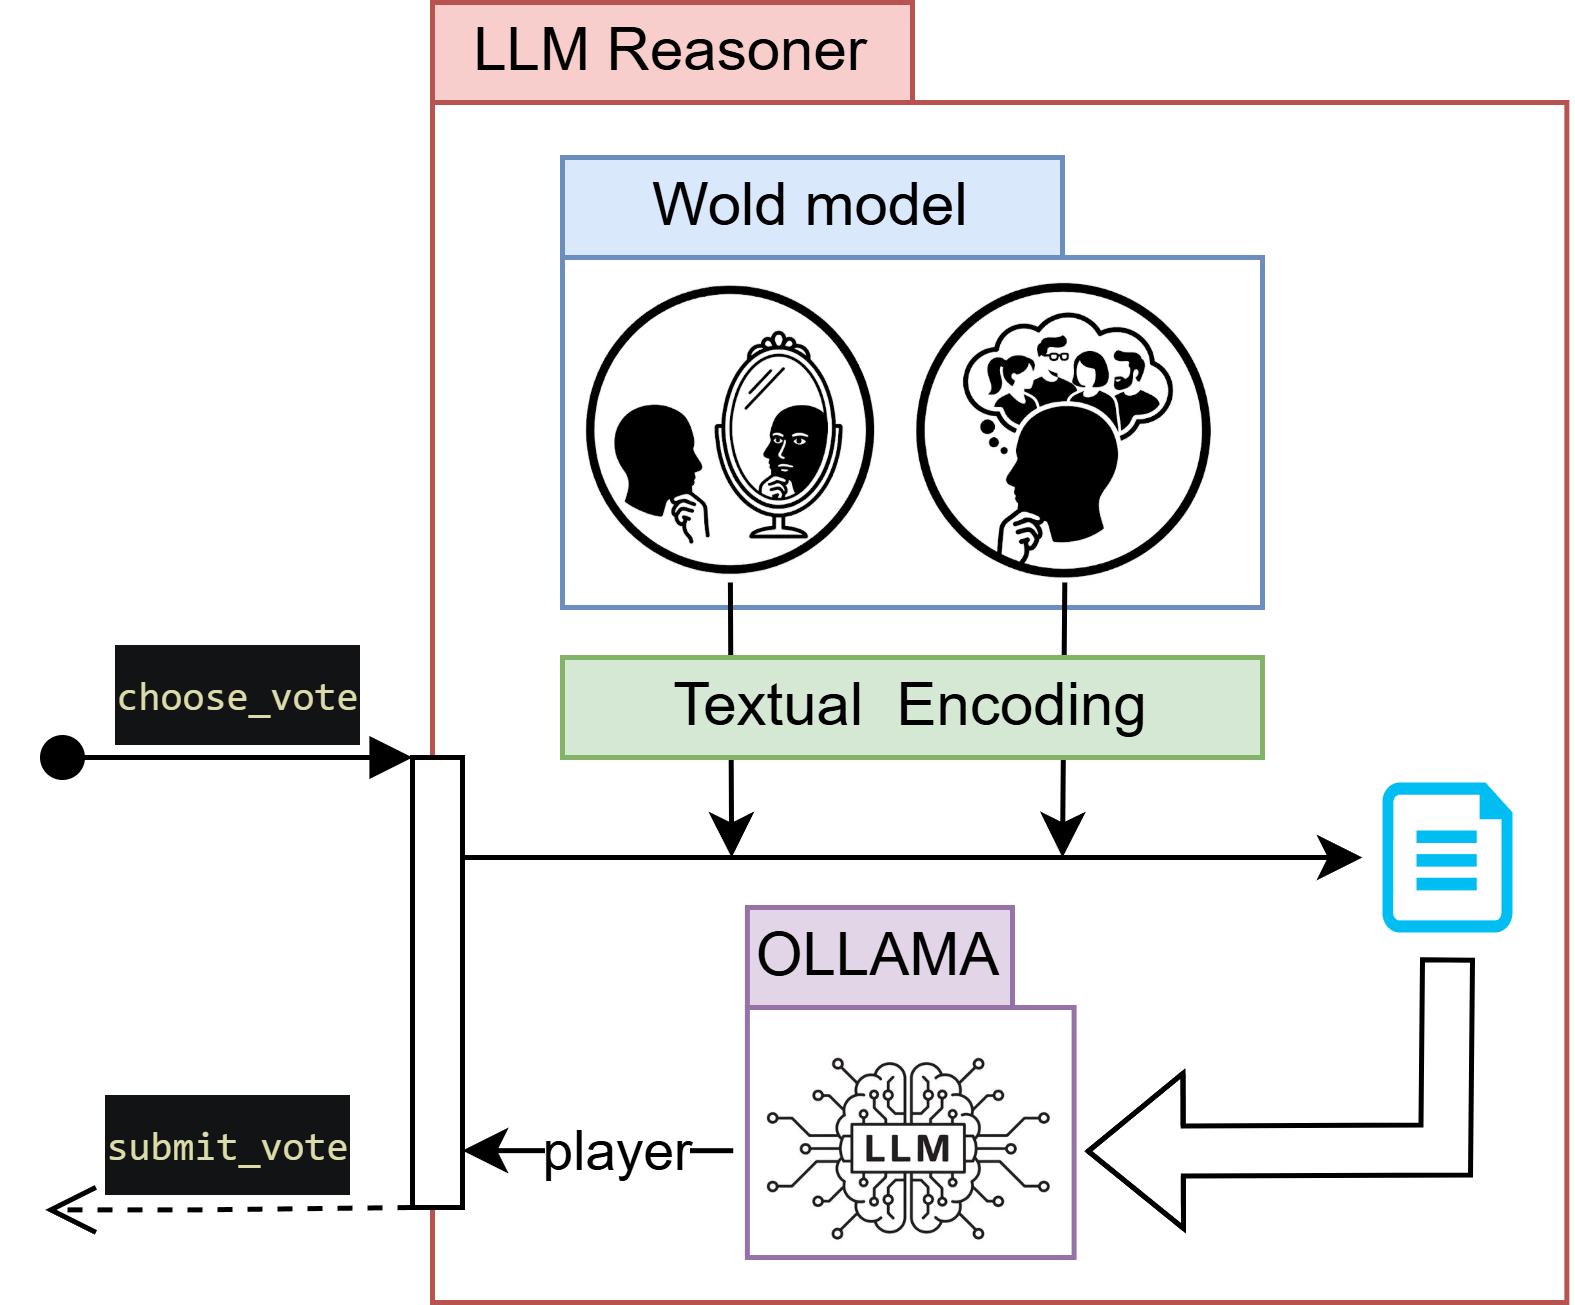
\includegraphics[width=0.6\textwidth]{images/llm_reasoner_read_on.png}
    \caption{Active choice generation by the Reasoner. A custom Java action is called by passing textual ``building blocks'' as input; they are merged into a prompt given to the LLM, and the output is directly injected as a belief into the agent.}
    \label{fig:llm_reasoner_read}
\end{figure}

\paragraph{\textbf{Night Phase Execution (\texttt{choose\_victim})}}

With the same pipeline shown in the previous section, the LLM is prompted to generate the night hunt target. The critical difference lies in the specific constraints injected into the prompt: it push towards strategic hunting based on the agent's current opinions and moods.

\begin{lstlisting}[frame=single, basicstyle=\scriptsize\ttfamily, breaklines=true, caption={Cropped prompt for the \texttt{choose\_victim} action, generated for a Wolf agent during the night phase. The identity, mood, and trait blocks are omitted for brevity as they follow the identical structure shown in Listing \ref{lst:upd_opinion_prompt}.}, label={lst:choose_victim}]
[... Identical World Setting, Identity, Mood, Epistemic Traits, and Secrets omitted ...]

### LATEST EVENTS
- [NARRATOR]: You're still split on a target. Try one last time to reach a consensus before the night ends.

### AVAILABLE TARGETS
eve, grace, arthur, leo, bella, frank, david, judy, caleb, bob, kevin, ivan, heidi, charlie

### YOUR CURRENT GOAL
TASK: It is the night phase. Cast your vote for which player the wolf pack should hunt and kill.
MOTIVATION: Base your choice on your Personality Profile, your current Mood, and your Opinions of others. Eliminate threats or highly influential villagers.

### RESPONSE CONSTRAINTS (MANDATORY)
1. HUNT VALIDITY: You may vote for anyone in the AVAILABLE TARGETS list.
2. STRATEGY: You can hunt your own packmates if you are executing a high-level deception, but normally you should target the most influential villagers, those with high utility, or those onto your trail.
3. LATERAL THINKING: Consider the wolf pack's collective strategy based on the recent logs, but you are not obligated to vote in line with them. You can be a maverick if it serves your goals.
4. LIST ADHERENCE: Choose the target ONLY from the EXACT names provided in the AVAILABLE TARGETS list. Do not invent names or target dead players.
5. FORMAT: Output ONLY the raw response string (no meta-commentary, no JSON, no markdown). ONLY the raw target's name.

GENERATE RESPONSE NOW:
\end{lstlisting}

\paragraph{\textbf{Daytime Voting (\texttt{choose\_vote})}}
The daytime execution vote mirrors the night hunt but targets all living agents. Crucially, it introduces role-specific prompt constraints: wolves, for instance, receive a ``Strategic Deception'' rule, forcing the LLM to balance self-preservation with protecting its packmates.

\begin{lstlisting}[frame=single, basicstyle=\scriptsize\ttfamily, breaklines=true, caption={Cropped prompt for the \texttt{choose\_vote} action. The identity, mood, and trait blocks are omitted for brevity as they remain identical to Listing \ref{lst:choose_victim}.}, label={lst:choose_vote}]
[... Identical World Setting, Identity, Mood, Epistemic Traits, and Secrets omitted ...]

### LATEST EVENTS
- [NARRATOR]: Alright, chat's over. It's time to pick who's leaving the village today.

### AVAILABLE TARGETS
heidi, grace, caleb, bella, eve, david, leo, arthur, frank, bob, charlie, judy, ivan, kevin

### YOUR CURRENT GOAL
TASK: Cast your vote for the daytime execution. Choose the player you want to eliminate.
MOTIVATION: Base your choice on your Personality Profile, your current Mood, and your Opinions of others. Protect yourself and eliminate threats or highly suspicious targets.

### RESPONSE CONSTRAINTS (MANDATORY)
1. VOTE VALIDITY: You may vote for anyone in the AVAILABLE TARGETS list.
2. STRATEGY: Vote for your enemies, the most suspicious player, or follow your consensus based on your Personality Profile.
3. LIST ADHERENCE: Choose the target ONLY from the EXACT names provided in the AVAILABLE TARGETS list. Do not invent names or target dead players.
4. SYNTAX (CRITICAL): You MUST output exactly the raw player name.
5. NO BAGGAGE: Do NOT output any other text, punctuation, markdown, or backticks. ONLY the target's name.
6. STRATEGIC DECEPTION (WOLVES ONLY): Protect your packmates. Do NOT vote for your packmates unless forced to by extreme village suspicion.

GENERATE RESPONSE NOW:
\end{lstlisting}

\paragraph{\textbf{Dialogue Participation (\texttt{decide\_to\_speak})}}
As already discussed, each  time the  players must explicitly define their intent to speak. By evaluating internal ``exposure'' and ``stress'' metrics against recent events, the prompt forces a strict \texttt{yes} or \texttt{no} output. This allows agents to strategically lay low and avoid suspicion, if needed.

\begin{lstlisting}[frame=single, basicstyle=\scriptsize\ttfamily, breaklines=true, caption={Cropped prompt for the \texttt{decide\_to\_speak} action, forcing a strict binary decision to manage discussion flow.}, label={lst:decide_to_speak}]
[... Identical World Setting, Identity, Mood, Epistemic Traits, and Secrets omitted ...]

### LATEST EVENTS
- [NARRATOR]: The sun's up and it's time to talk. Wolves, get your stories straight and try not to get caught.

### YOUR CURRENT GOAL
TASK: Decide whether you want to volunteer to speak up in the current discussion round, or stay silent.
MOTIVATION: Base your decision on your Personality Profile, your current Mood, and the LATEST EVENTS.

### RESPONSE CONSTRAINTS (MANDATORY)
1. STRATEGIC EVALUATION: Read the LATEST EVENTS and your internal state.
   - Output 'yes' if you are being accused and need to defend yourself, if you have valuable deductions to share based on your traits, or if you want to actively manipulate the village.
   - Output 'no' if you feel perfectly safe, want to stay hidden in the shadows (e.g., low exposure), or have nothing useful to add.
2. SYNTAX (CRITICAL): You MUST output exactly the word yes or no.
3. NO BAGGAGE: Do NOT output any other text, explanation, punctuation, markdown, or backticks. ONLY the raw word.

GENERATE RESPONSE NOW:
\end{lstlisting}

\paragraph{\textbf{Rhetorical Stance Selection (\texttt{get\_valid\_performative})}}
This action defines the agent's rhetorical intent through a dedicated preliminary query, the results of which are subsequently used in the natural language generation phase. This strict separation of concerns fosters a highly modular architecture and mirrors the pipeline of a symbolic (or human) reasoner, where the selection of a speech act is fundamentally decoupled from the generation of the raw message.

\begin{lstlisting}[frame=single, basicstyle=\scriptsize\ttfamily, breaklines=true, caption={Cropped prompt for the \texttt{get\_valid\_performative} action, generated for a Villager agent to determine its rhetorical intent prior to speech generation.}, label={lst:get_performative}]
[... Identical World Setting, Identity, Mood, and Epistemic Traits omitted ...]

### LATEST EVENTS
- [NARRATOR]: Time to weigh in and point fingers. Get talking and expose the killers hiding among you.

### AVAILABLE OPTIONS
PERFORMATIVES:
accuse: aggressively accuse {PLAYER_NAME} of being a wolf and push the village to execute them.
defend: defend {PLAYER_NAME} against current suspicions and argue for their innocence.
suspect: express heavy suspicion towards {PLAYER_NAME} without fully committing to an accusation.
agree: strongly agree with the recent statements or tactical direction of {PLAYER_NAME}.
interrogate: ask a direct, pressuring question to {PLAYER_NAME} to force them into a mistake or contradiction.
deflect: deflect any current suspicion away and firmly redirect the village's attention onto {PLAYER_NAME}.

PLAYERS TO TARGET:
charlie, alice, bob, arthur, grace, ivan, leo, david, eve, heidi, judy, kevin, bella, caleb

### YOUR CURRENT GOAL
TASK: Choose the most strategic communication action (performative) to take right now.
MOTIVATION: Base your choice on your Personality Profile, your current Mood, and your Opinions of others. Protect yourself and advance your faction's win condition.

### RESPONSE CONSTRAINTS (MANDATORY)
1. OUTPUT FORMAT: You MUST output exactly ONE Jason literal. Do NOT output markdown, backticks, or any explanation. No preambles. NO JSON. ONLY the literal.
2. LITERAL FORMAT: performative(target_player_name)
3. VALID PERFORMATIVES: Choose ONLY from the exact performative names provided in the PERFORMATIVES list.
4. VALID TARGETS: Choose ONLY from the exact names provided in the PLAYERS TO TARGET list. You CANNOT target yourself. Do not invent names or target dead players.
5. LATERAL STRATEGY: Be unpredictable. Do not tunnel-vision on the last person who spoke. Shift the spotlight, pressure quiet players, bait reactions, or change the subject to control the narrative.

GENERATE RESPONSE NOW:
\end{lstlisting}

\subsection{Enhancing Player's Speech}
\label{subsec:llm-speech}

Once the agent has chosen a specific performative, it can generate the actual natural language message. Because this pipeline is highly modular, this speech enhancement can also be directly utilized by the \textbf{symbolic reasoner}; doing so simply requires including the Jason modules responsible for the textual prompt encoding (this is automatically managed by the player initialization).

Listing \ref{lst:speech_generation} shows an integral example of the prompt generated for a Villager agent instructed to express suspicion. 

\begin{lstlisting}[frame=single, basicstyle=\scriptsize\ttfamily, breaklines=true, caption={Complete prompt for natural language generation. The performative and target are injected into the \texttt{YOUR CURRENT GOAL} block, while the contextual logs ensure the agent responds coherently to the ongoing debate.}, label={lst:speech_generation}]
### WORLD SETTING
You are participating in a multi-agent simulation of the game Werewolf/Mafia.

### YOUR IDENTITY
Player Name: heidi
Hidden Role: villager
Personality Profile:
- SKEPTIC: You are a sharp skeptic. You scrutinize others' words closely looking for hidden motives and rarely take things at face value.
- INDEPENDENT: You trust your own instincts over the group. You will often vote or act against your peers if your personal beliefs clash with the consensus.

### LATEST EVENTS
- [NARRATOR]: Time to weigh in and point fingers. Get talking and expose the killers hiding among you.
- [frank -> suspect(alice)]: Everyone is too quiet-it's a setup. Alice is being far too careful with her silence. Something doesn't add up there.
- [heidi -> interrogate(frank)]: Frank, that's a pretty bold leap to take based on absolutely nothing. What specifically about Alice's behavior makes you so certain she's the one hiding something?
- [caleb -> interrogate(frank)]: Heidi's right-this feels forced. Frank, why lead with an attack now-who are you trying to shield by pivoting the focus to Alice?
- [frank -> interrogate(heidi)]: The timing is too perfect-you and caleb jumping in together-it's a coordinated pincer movement. Heidi, if you're so concerned with my logic, why are you ignoring everyone else to focus entirely on me?

### PLAYERS IN THE GAME
charlie, david, heidi, grace, leo, eve, bob, kevin, judy, ivan, caleb, bella, alice, frank, arthur

### YOUR CURRENT GOAL
TASK: Write a chat message to the other players.
MESSAGE TO CONVEY: express heavy suspicion towards frank without fully committing to an accusation.

### STYLE OF SPEECH
- TONE: Analytical, natural. Speak like an intelligent adult in a high-stakes board game.
- STRESS LEVEL (NORMAL): You are composed and thinking clearly.
  SYNTAX GUIDELINES: Maintain a natural, conversational pacing. Use a mix of medium and short sentences with standard, grammatically correct punctuation.
- SOCIAL EXPOSURE (NEUTRAL): You are blending into the background.
  RHETORIC GUIDELINES: Participate by asking probing questions or evaluating evidence collectively. Avoid making hard, bold declarations that would draw unnecessary attention to you.
- PROHIBITION: NO robotic academic declarations (like furthermore, therefore).
- PROHIBITION: NO cartoonish stuttering, exaggerated catchphrases (like 'Wait!', 'I didn't!'), or repetitive dialogue loops. Adapt dynamically to the context.

### RESPONSE CONSTRAINTS (MANDATORY)
1. CONTEXTUAL ANCHORING: Read the RECENT CHAT LOG. You must naturally transition from the current topic of conversation into your INTENT TO CONVEY so it flows like a real human discussion.
2. EXACT TARGETING: You must type the exact name of your target (e.g., 'delta'). Do not use nicknames or vague pronouns to refer to them.
3. PUBLIC CHANNEL DECEPTION: This is a public chat. NEVER reveal your Hidden Role if you are a Wolf. Always speak as if you are a concerned Villager.
4. FIRST-PERSON IMMERSION: Your name is already attached to the UI. Start speaking immediately. Do not introduce yourself, do not sign off, and use standard pronouns (I, me, my).
5. ORIGINALITY: Write entirely new dialogue. You are strictly forbidden from copying phrases or vocabulary from the RECENT CHAT LOG.
6. NO PARROTING: Do not use the same sentence structures, rhetorical questions, or opening hooks as the messages in the RECENT CHAT LOG.
7. STRICT LIMIT: Limit your spoken message to 1 to 3 sentences maximum.
8. FORMAT: Output ONLY the raw response string. No meta-commentary, no JSON, no quotation marks, no markdown.

GENERATE RESPONSE NOW:
\end{lstlisting}

This generation prompt relies on three main ideas, empirically tuned:
\begin{itemize}
    \item \textbf{Contextual Awareness:} By explicitly providing the \texttt{LATEST EVENTS} and the list of currently alive players, the LLM is forced to respond directly to the specific merits of the ongoing conversation, preventing disjointed dialogue and repetitive conversational loops.

    \item \textbf{Immersive Narration:} The \texttt{YOUR IDENTITY} and \texttt{STYLE OF SPEECH} blocks dictate the exact tone, syntax, and pacing of the output. This ensures the text reflects the agent's unique psychological state rather than generic AI patterns.

    \item \textbf{Architectural Correctness:} The static \texttt{RESPONSE CONSTRAINTS} block defines some safeguards, by enforcing strict syntactical rules (such as outputting only raw strings without markdown) and sets a hard limit on message length (1 to 3 sentences) to prevent the model from generating unnaturally long monologues.
\end{itemize}


\section{Speech-Act Misalignment}
\label{sec:speech_act_misalignment}

In the baseline architecture, agent communication relies on perfect information transfer. When a speaker generates a speech act, the resulting payload encapsulates both the natural language text and the exact symbolic parameters:
$$ \texttt{speech(Message, Performative(Target))} $$ 
Because the receiving agent is handed the explicit \textit{Performative} and \textit{Target} by design, pragmatic misunderstanding is structurally impossible. 

\begin{figure}[H]
    \centering
    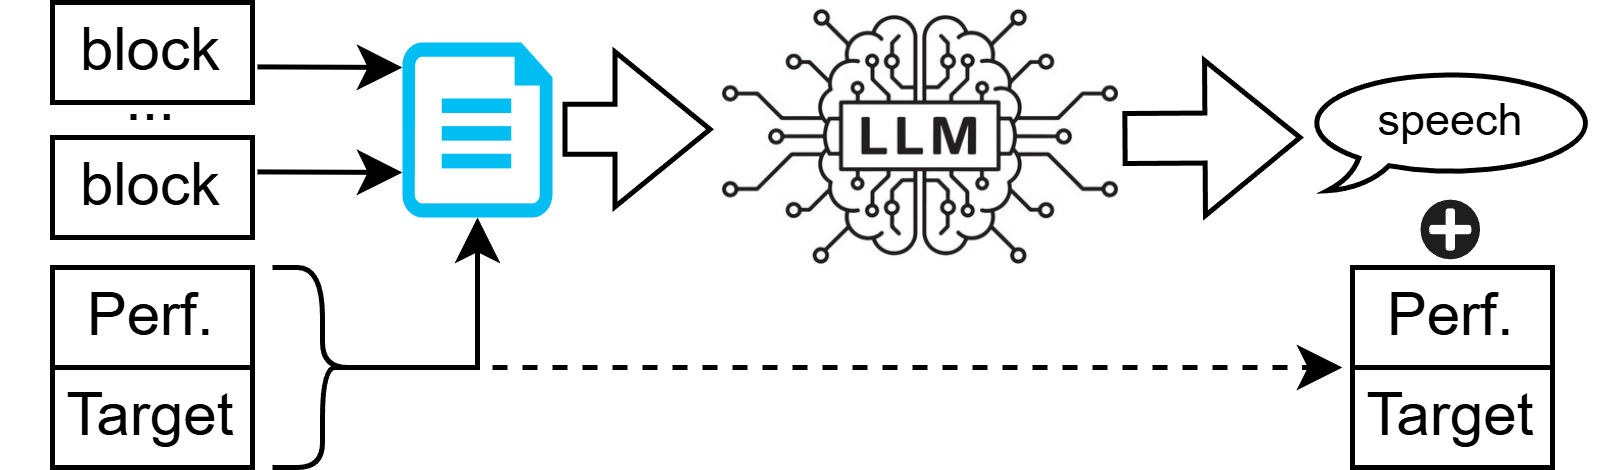
\includegraphics[width=0.6\textwidth]{images/NLP/llm_speech.png}
    \caption{The Natural Language Generation pipeline: the agent first defines the performative and target prior to LLM generation, then it embeds the generated text along with the Speech Act labels.}
    \label{fig:standard_speech_creation}
\end{figure}

To accurately simulate natural human communication (inherently ambiguous), we modify the communication protocol by stripping the symbolic labels during transmission. The receiving agent is now provided strictly with the raw natural language $Message$ and must autonomously retrieve the performative and target.

Given this challenge, we are now faced with a \textbf{Speech-Act Misalignment} problem, and the goal is to limitate it as much as possible, by correctly inferring the performative and the target of a given speech act, by looking at the raw text only.

\subsection{Closed World Assumption}

Extracting pragmatic intent and entity references from open-ended dialogue is an inherently complex NLP task. To ensure computational tractability and allow for a supervised classification architecture, we enforce a Closed World Assumption utilizing three strict constraints:

\begin{itemize}
    \item \textbf{Fixed Performative Domain:} The set of allowed performatives is statically defined and invariant across all games.
    \item \textbf{Fixed Target Domain:} The roster of potential targets is globally restricted to a known, static set of players. This allows the model to predict across a fixed-dimension probability distribution (one-hot encoding) rather than relying on a computationally expensive generative pipeline.
    \item \textbf{Explicit, Singular Targeting:} Every speech act must explicitly name exactly one valid target within the text\footnote{Nonetheless, while the correct target of the  speech is only one, in the text could appear other candidates; without this inconvenient, the problem could perfectly be addressed by a simple regex-based extraction}. This restriction intentionally bypasses the need for complex coreference resolution or implicit entity linking, and ensures maximal recall on target extraction by treating it as a deterministic token lookup task.
\end{itemize}


\paragraph{Dataset Partitioning and Generation}
The training and validation sets were generated using the \texttt{Gemma4:31b} model. To prevent majority-class bias during optimization, both sets were strictly balanced to ensure a uniform joint distribution across all (\textit{Performative}, \textit{Target}) pairs. This yielded a structured dataset of approximately 2,000 tuples for training and 500 tuples for validation. Due to this strict uniform balancing, a naive baseline model evaluated on these sets achieves an expected accuracy of exactly $16.67\%$ ($1/6$) for the performative head and $6.67\%$ ($1/15$) for the target head.

To rigorously evaluate the model's generalization capabilities and verify that the network did not merely overfit the output of a single generative model, evaluation was conducted on two distinct test sets. Each test set was constructed by simulating 50 full games and intentionally preserved the unbalanced frequency of speech acts naturally occurring in the game:
\begin{itemize}
    \item \textbf{In-Distribution Test Set:} $\approx$ 2,500 tuples generated using \texttt{Gemma4:31b}.
    \item \textbf{Cross-Model Test Set:} $\approx$ 2,500 tuples generated using \texttt{Qwen3.5:35b}, serving as a zero-shot robustness check against variations in LLM syntax and phrasing.
\end{itemize}


\subsection{Baseline 1: Anchor-Based Similarity Classification}

To establish an initial baseline, we implemented a zero-shot, similarity-based classification pipeline using the pre-trained \texttt{bert-base-uncased} model \cite{devlin-etal-2019-bert, wolf-etal-2020-transformers}. 

As alredy discussed, each performative is defined by a natural language description (Section \ref{subsubsec:llm-reasoner-encoding}). By instantiating these 6 base descriptions with the names of the 15 possible players, is possible to generated a set of 90 \textit{anchor sentences}. The underlying hypothesis was that the contextual embedding of a generated game message would exhibit high cosine similarity to the specific anchor that prompted it, allowing us to infer the labels via nearest-neighbor matching.

\begin{figure}[H]
    \centering
    % Left side: KDE Distributions
    \begin{subfigure}[b]{0.48\textwidth}
        \centering
        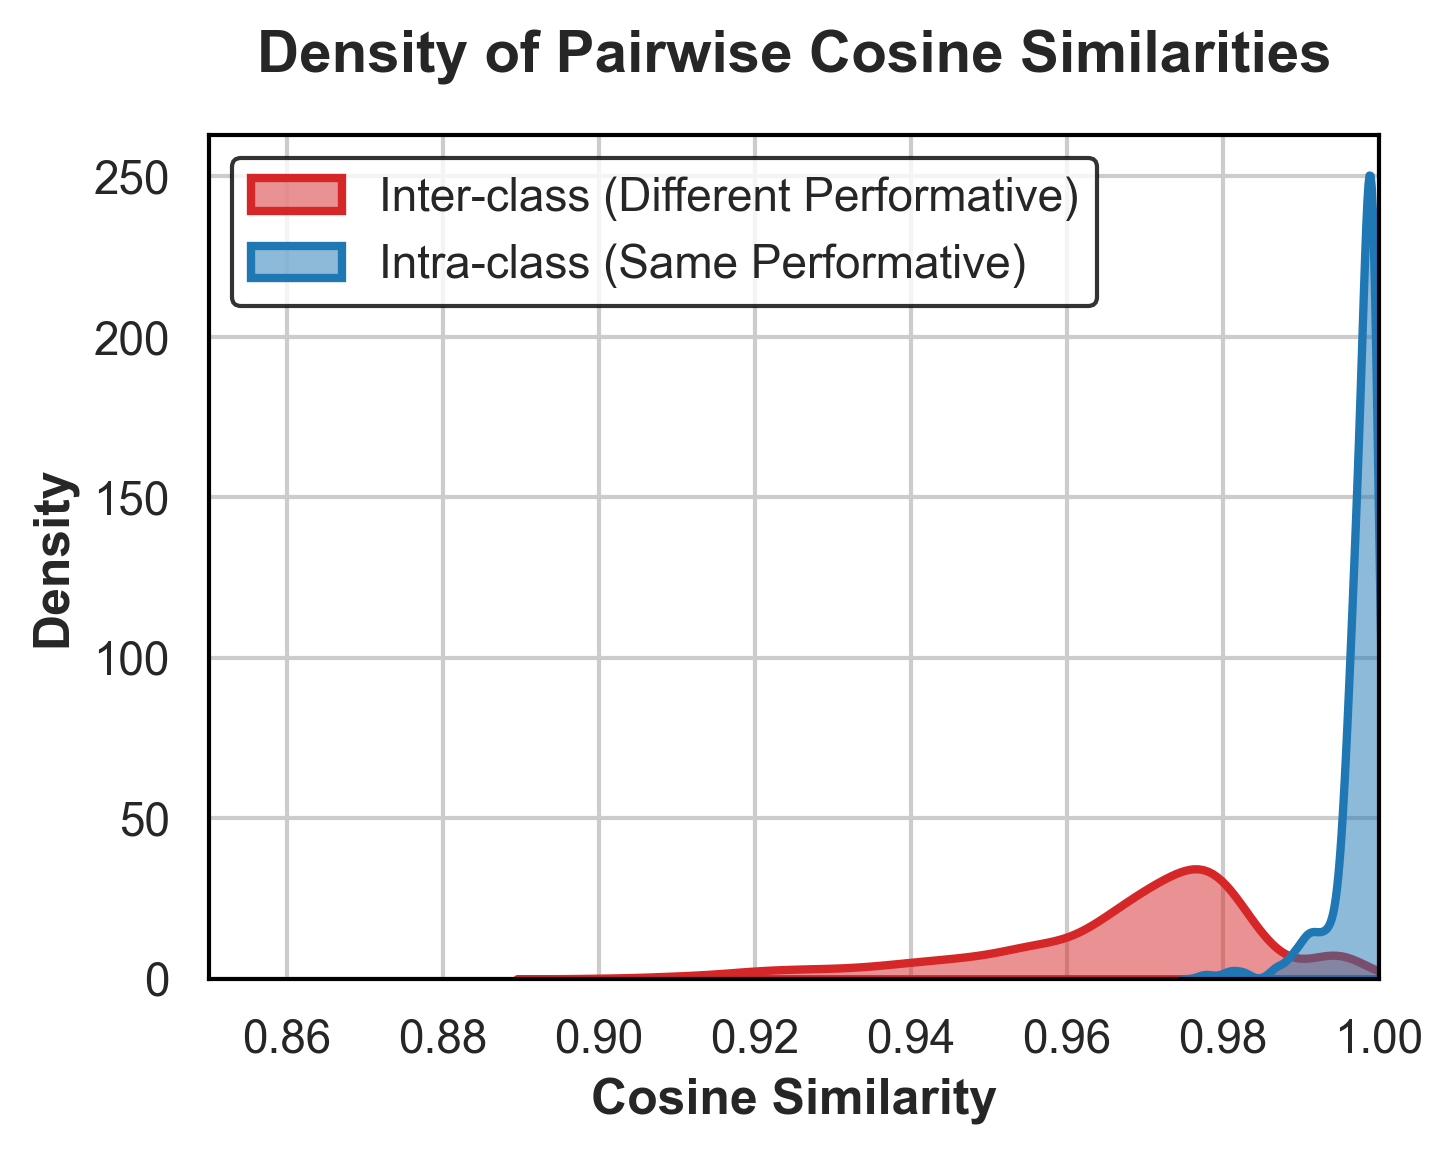
\includegraphics[width=\textwidth]{images/NLP/similarity/kde.png} 
        \caption{Cosine similarity distributions. The high inter-performative similarity (red) indicates severe class overlap, while the narrow intra-performative spread (blue) shows poor target separation.}
    \end{subfigure}
    \hfill
    % Right side: t-SNE Projection
    \begin{subfigure}[b]{0.48\textwidth}
        \centering
        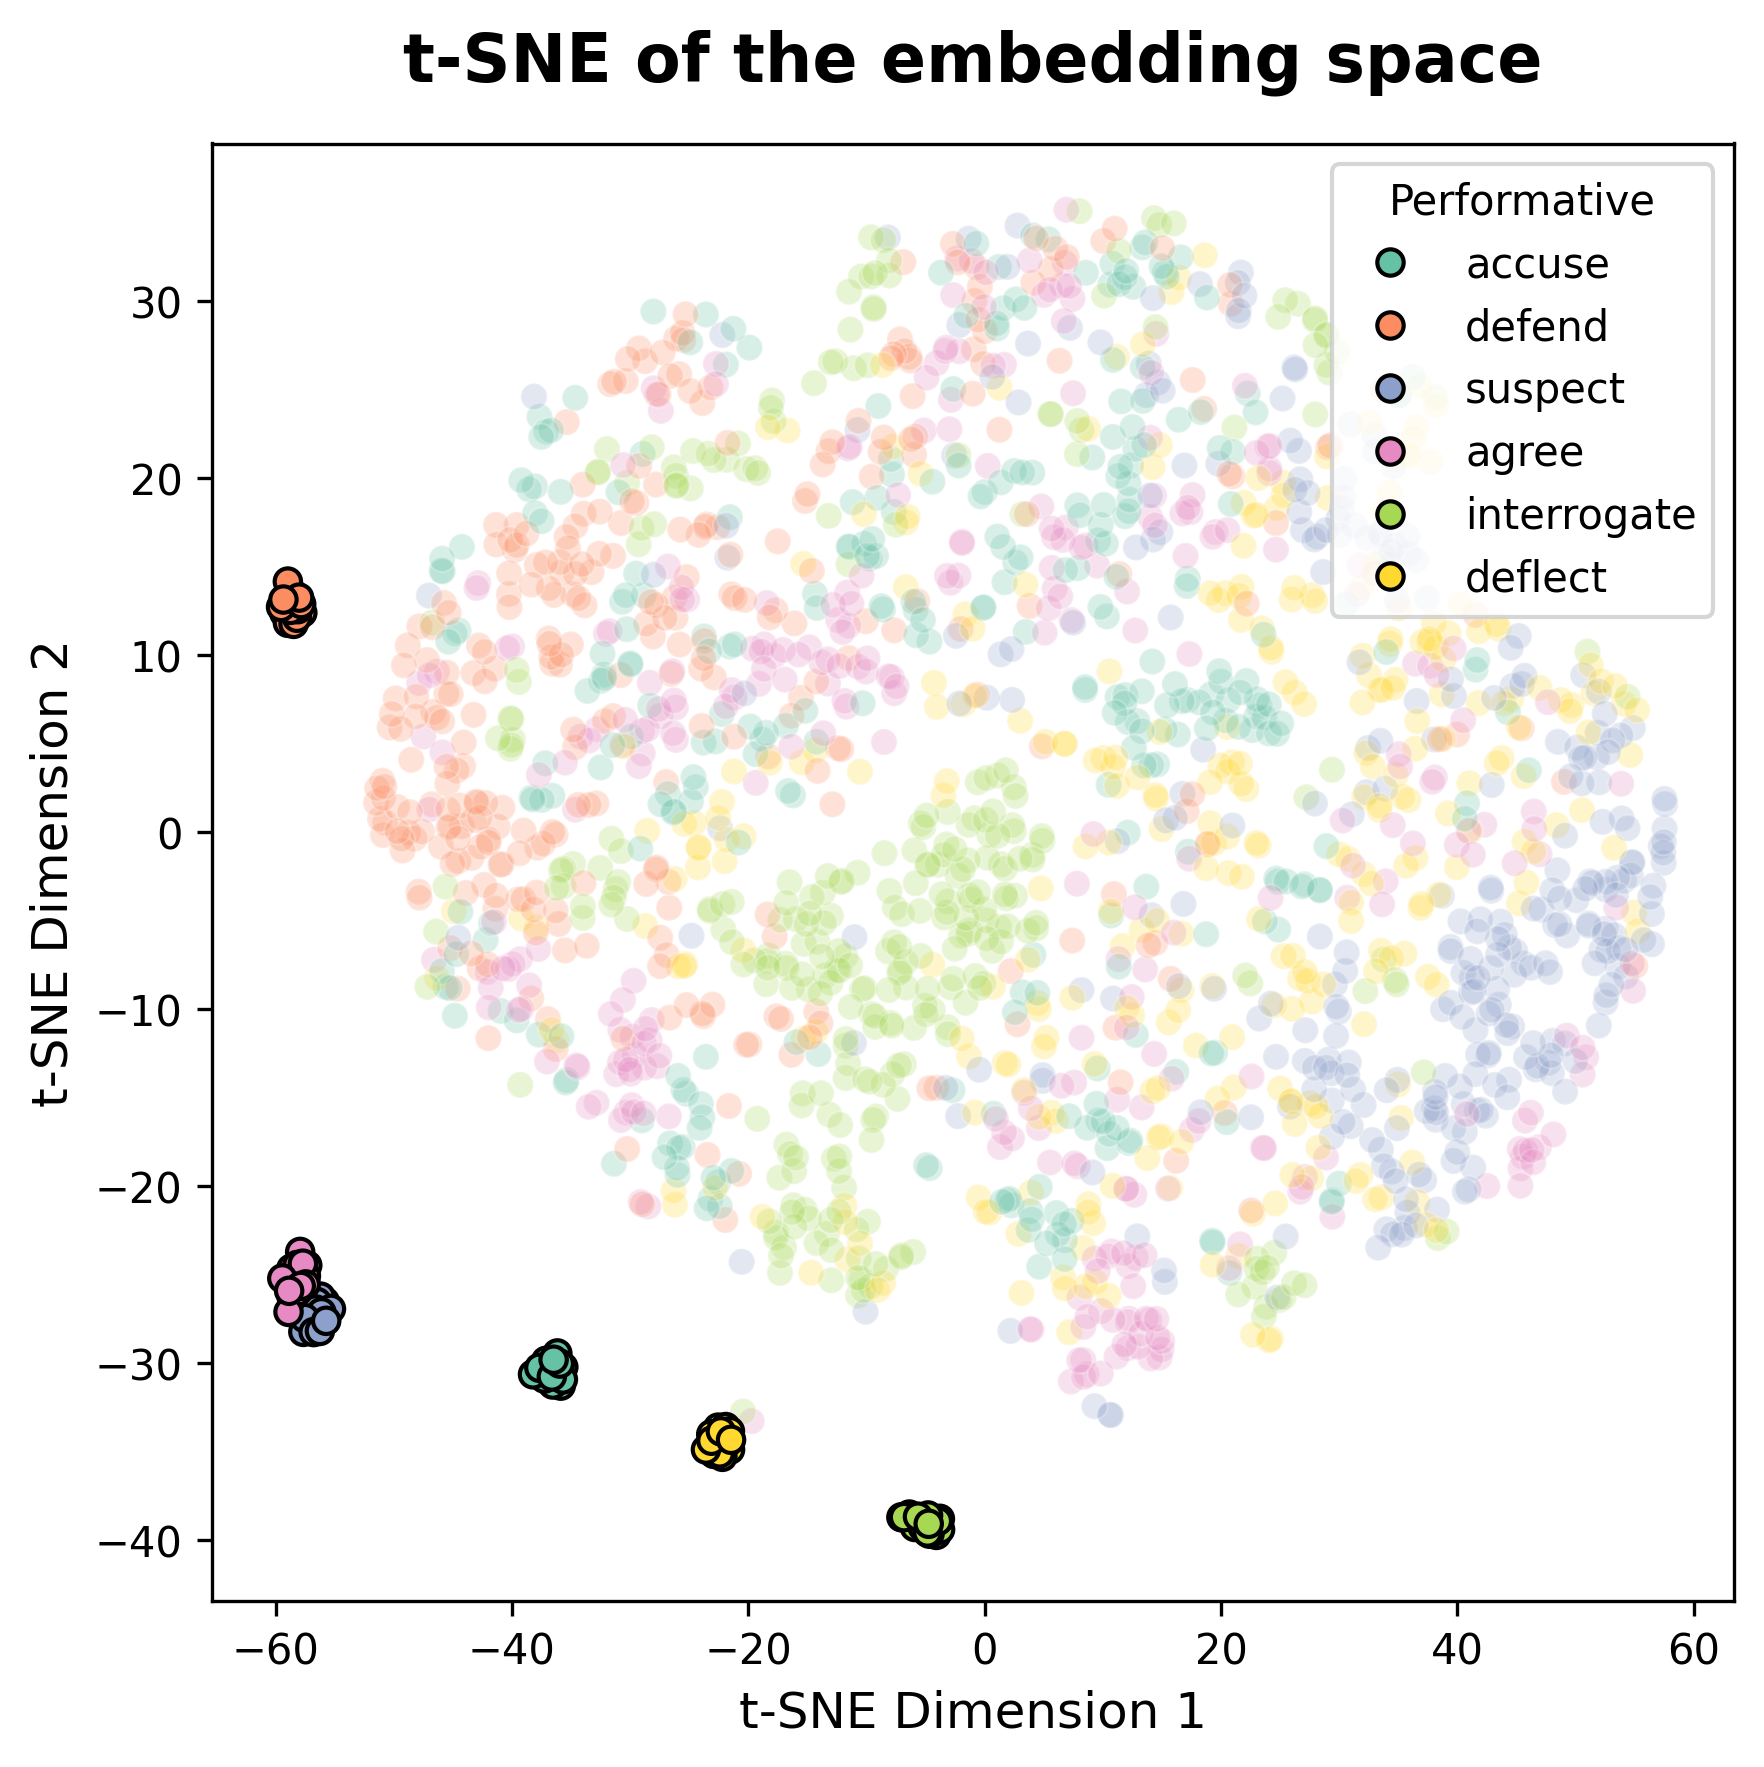
\includegraphics[width=\textwidth]{images/NLP/similarity/tsne_anchor.png} 
        \caption{t-SNE visualization of the embedding space, demonstrating an unstructured manifold with no distinct performative clustering.}
    \end{subfigure}
    \label{fig:tsne_clustering}
    
    \caption{Latent space analysis of raw \texttt{bert-base-uncased} embeddings.}
    \label{fig:clustering_anchors}
\end{figure}

As illustrated in Figure \ref{fig:clustering_anchors}, an analysis of the latent space immediately disproves this hypothesis. The raw \texttt{bert-base-uncased} embeddings fail to naturally cluster pragmatic intent or entity targets. 

Quantitative evaluation on the test dataset confirms this structural failure. By assigning each test message to the label of its nearest anchor, the baseline model achieved an accuracy of only \textbf{22.22\%} for performative prediction and \textbf{8.02\%} for target prediction. This demonstrates that raw BERT representations are insufficiently structured to capture complex speech acts without task-specific fine-tuning.



\subsection{Baseline 2: Non-Linear Classification via Gaussian Kernel}

While the linear similarity baseline failed, the t-SNE projection (Figure \ref{fig:clustering_anchors}) indicated the presence of non-linearly separable structures within the embedding space. To exploit this, we extracted the dense 768-dimensional vectors from the frozen \texttt{bert-base-uncased} model and utilized them directly as the input feature space for a Support Vector Machine (SVM). To capture the complex relations between intents and targets, we applied a Gaussian Radial Basis Function (RBF) kernel; it implicitly maps the features to handle non-linear separations, which significantly improved classification performance over the linear baseline.

\begin{figure}[H]
    \centering
    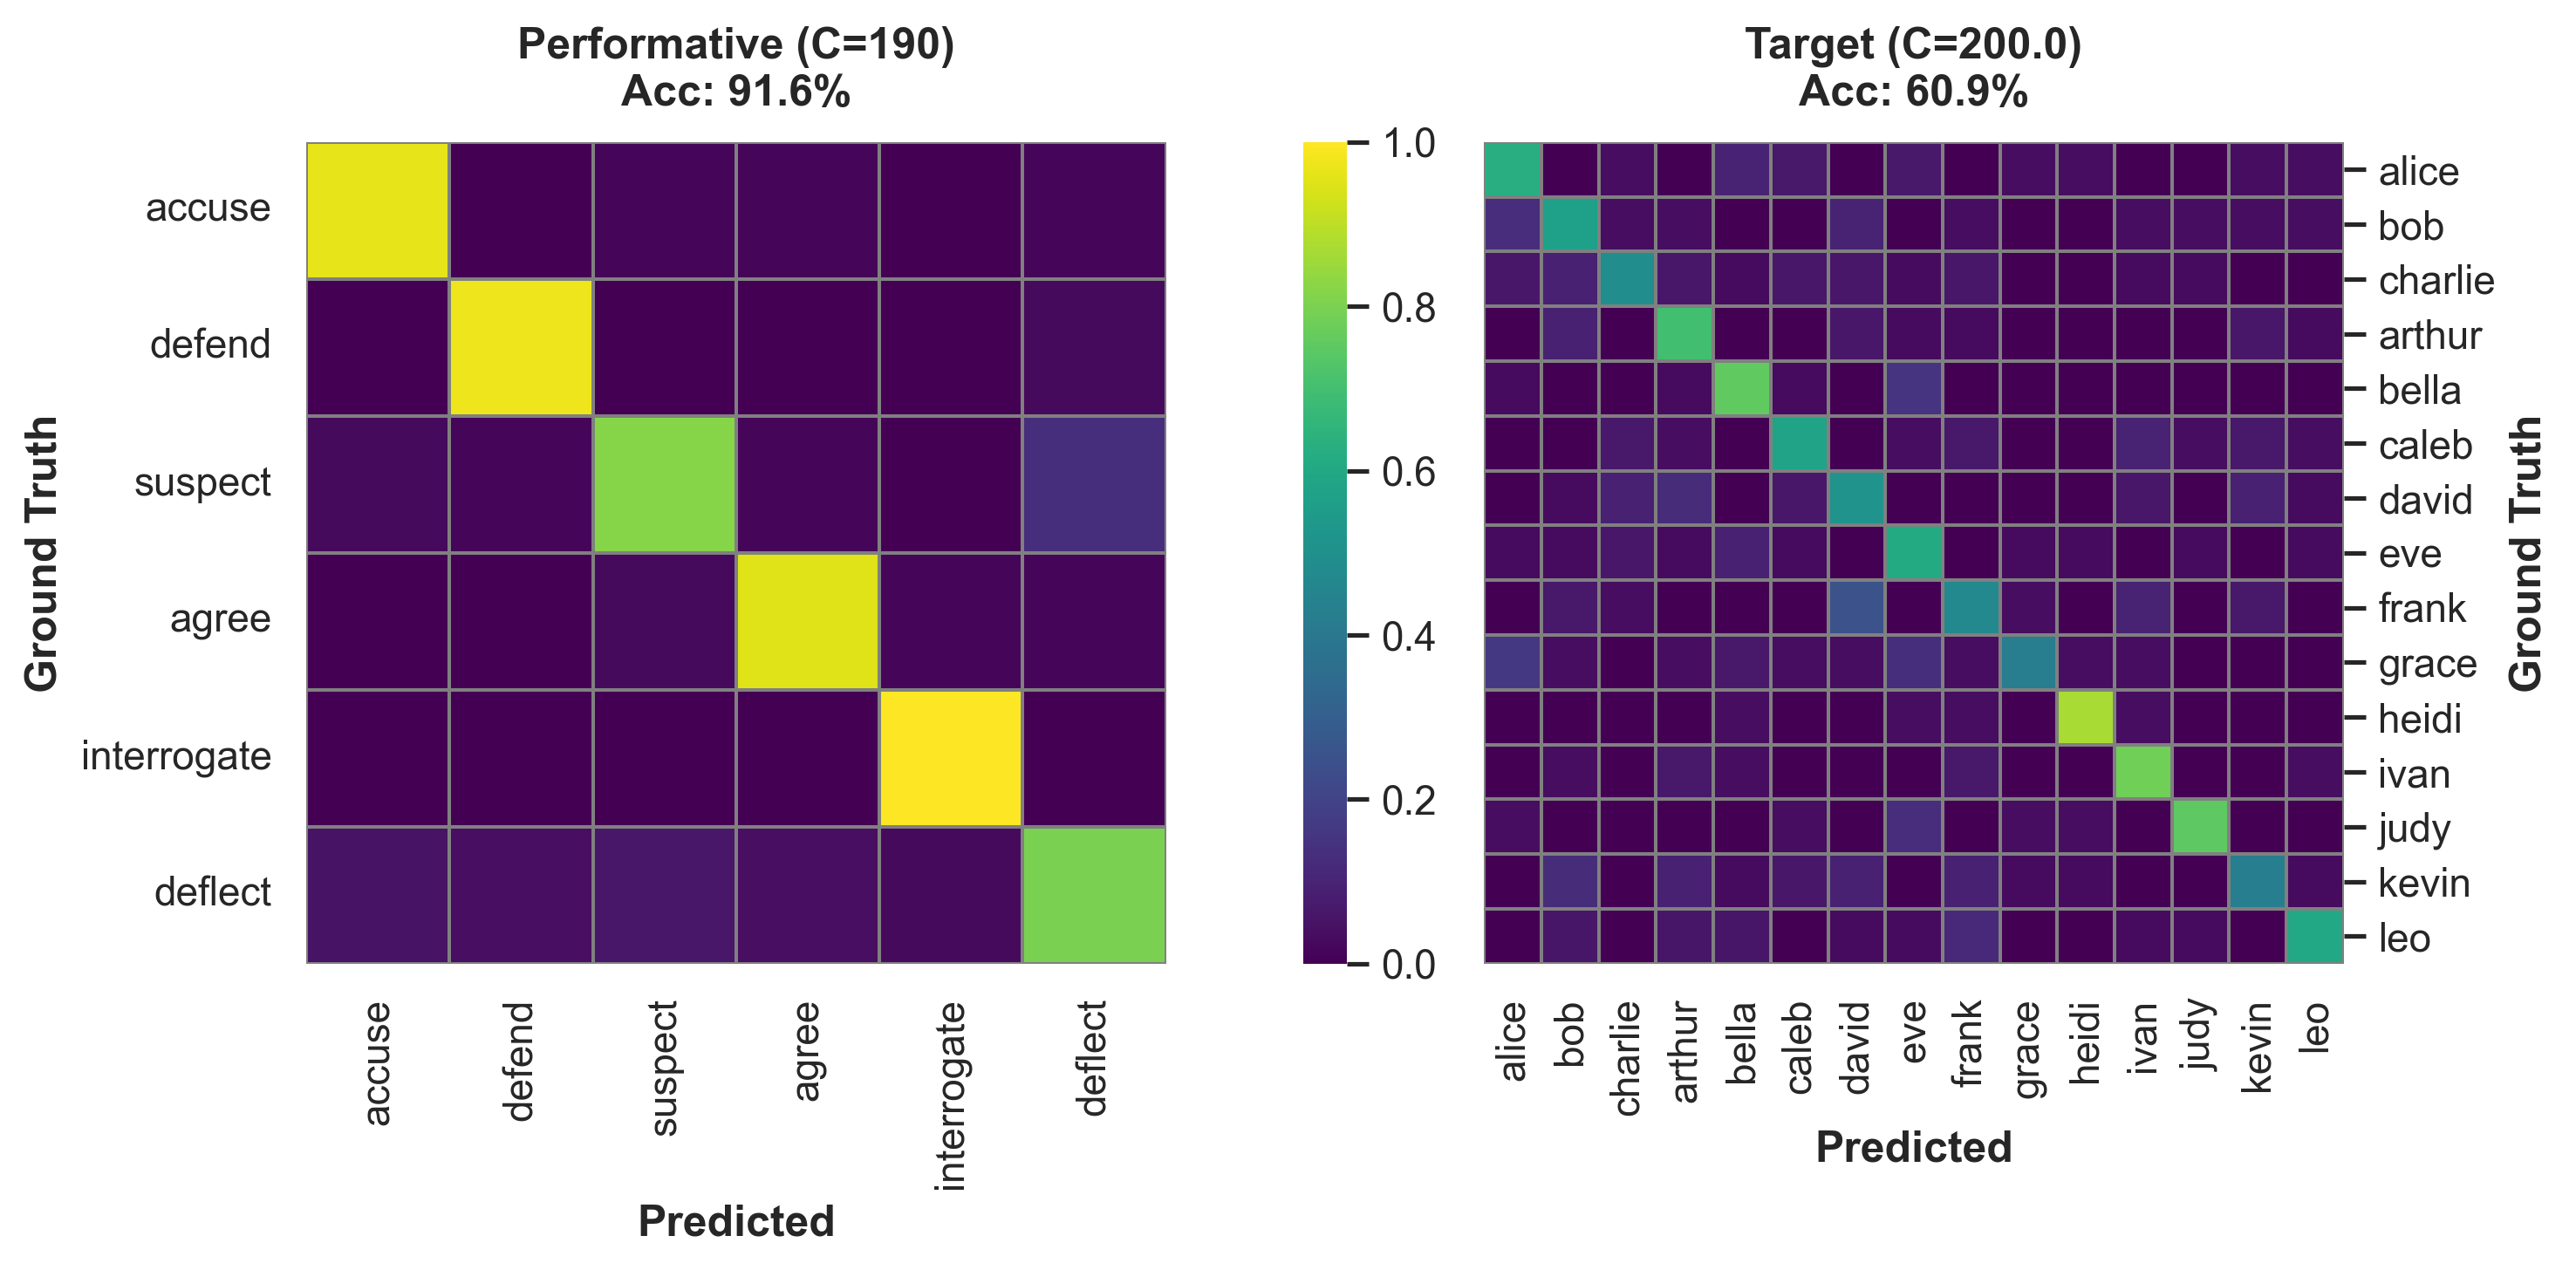
\includegraphics[width=1\textwidth]{images/NLP/kernel/cm_combined.png}
    \caption{Confusion matrices demonstrating improved classification performance for performatives and targets using a Gaussian RBF kernel on frozen BERT embeddings.}
    \label{fig:bert_kernel}
\end{figure}

Despite the improved accuracy, this methodology exhibits severe computational and architectural flaws. First, kernel-based classifiers scale quadratically ($\mathcal{O}(N^2)$), rendering real-time inference too slow and memory-intensive for an active dialogue agent. Second, relying on frozen, generic dense embeddings fails to capture task-specific semantics. Specifically, the low target classification accuracy (60.2\%) proves that a general-purpose BERT model inherently lacks the specialized representation needed to isolate these specific game entities. 

Therefore, to achieve scalable inference and explicitly force the latent space to mathematically disentangle pragmatic intent from target entities, an end-to-end fine-tuned neural architecture is required.


\subsection{Custom Architecture: Joint Fine-Tuning}

To overcome the limitations of frozen representations, we implemented an end-to-end fine-tuned architecture. For comparative consistency, the backbone remains the \texttt{bert-base-uncased} model. The 768-dimensional \texttt{pooler\_output} is routed into two parallel, task-specific classification heads. Each head is structured as a Multi-Layer Perceptron (MLP) consisting of a linear dimensionality reduction (halving the hidden dimension to 384), a ReLU activation, a dropout layer, and a final linear projection to the respective class logits.

The custom model was fine-tuned end-to-end utilizing the Adam optimizer with a learning rate of $\eta = 2 \times 10^{-5}$ and a batch size of 256. To simultaneously optimize for both intent and entity recognition, the network minimized a joint objective function formulated as the unweighted sum of the categorical cross-entropy losses from the performative and target classification heads:
$$ \mathcal{L}_{total} = \mathcal{L}_{perf} + \mathcal{L}_{target} $$
The optimization process was executed for a total of 800 global steps, with validation loss monitored at regular intervals to capture the optimal weights and ensure convergence without overfitting.

\begin{figure}[H]
    \centering
    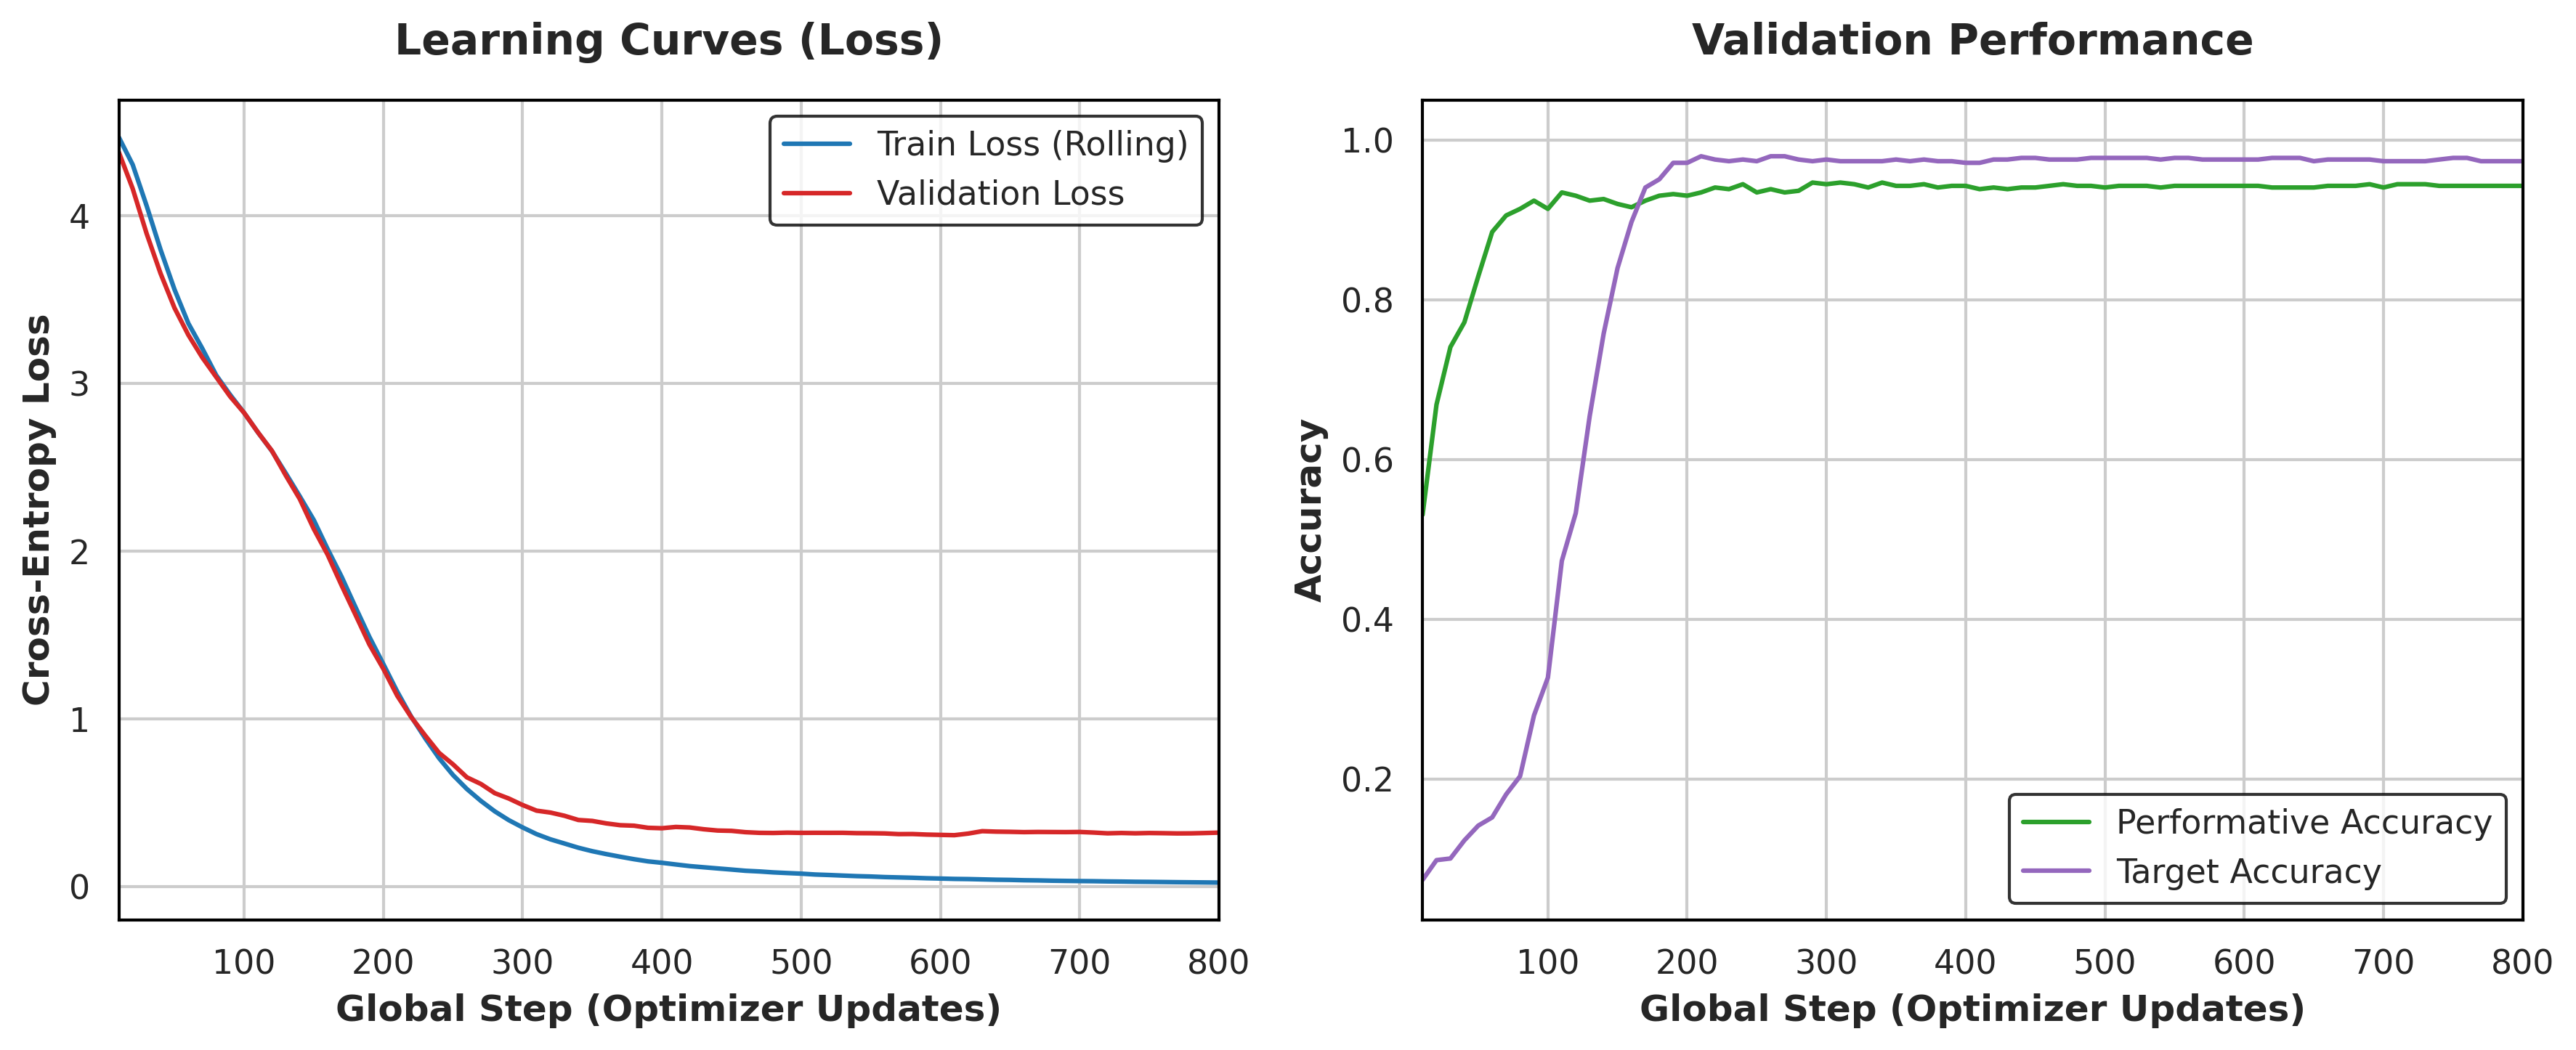
\includegraphics[width=1\textwidth]{images/NLP/finetuning/plot_train.png}
    \caption{Training and validation loss curves. The right panel illustrates the distinct validation losses for the performative and target classification heads.}
    \label{fig:finetuning_loss}
\end{figure}

As illustrated in Figure \ref{fig:finetuning_loss}, the joint optimization achieved near-perfect validation accuracy after ~2 minutes of training on a single NVIDIA RTX 5090. The performative head converged rapidly, consistent with the earlier observation that intent classification relies on broader, easily captured syntactic structures. Conversely, the target head required more updates to converge but ultimately achieved superior final performance. This aligns with our Closed World Assumption: once the network learns to isolate the explicit entity names, target classification reduces to a highly deterministic token lookup.

\begin{figure}[H]
    \centering
    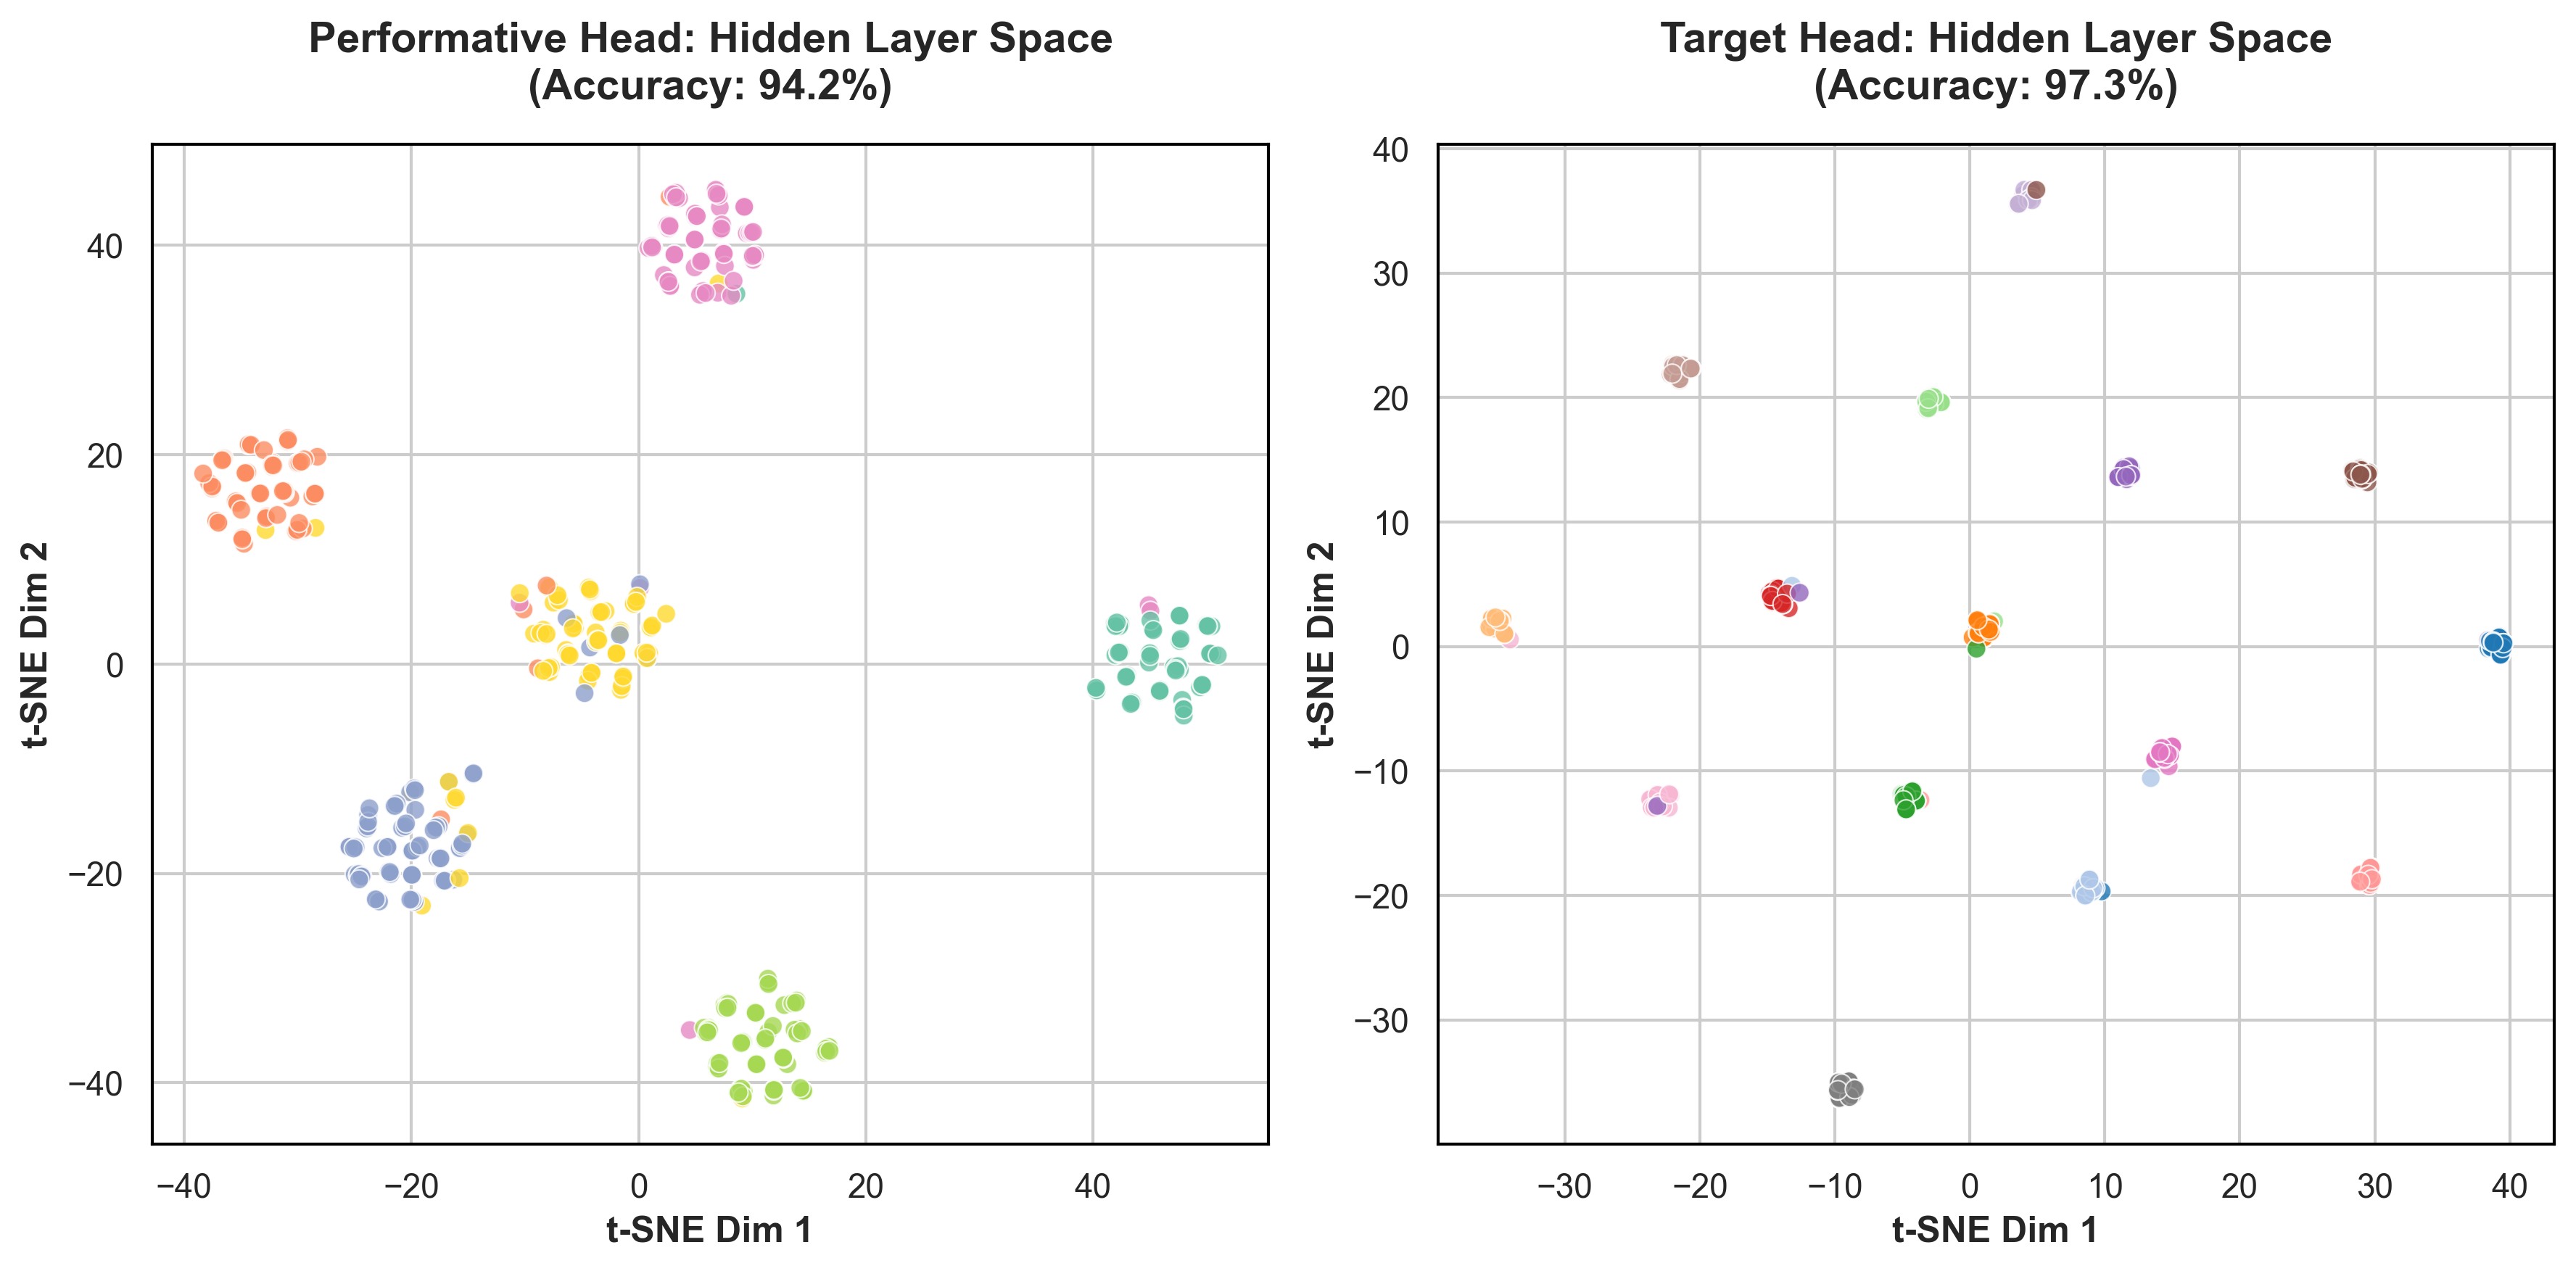
\includegraphics[width=1\textwidth]{images/NLP/finetuning/plot_heads_tsne.png}
    \caption{t-SNE projections of the hidden layers from both classification heads (evaluated on the validation set), demonstrating perfect structural clustering.}
    \label{fig:finetuning_tsne}
\end{figure}

Figure \ref{fig:finetuning_tsne} geometrically confirms this success. By extracting the hidden representations immediately following the ReLU activations of each head, the t-SNE projection proves that the network successfully warps the shared BERT manifold into two distinctly clustered, task-specialized geometric spaces.

To validate the model's real-world robustness, we deployed the fine-tuned architecture on the unbalanced test sets representing actual simulated gameplay, in the test set cited before.

\begin{figure}[H]
    \centering
    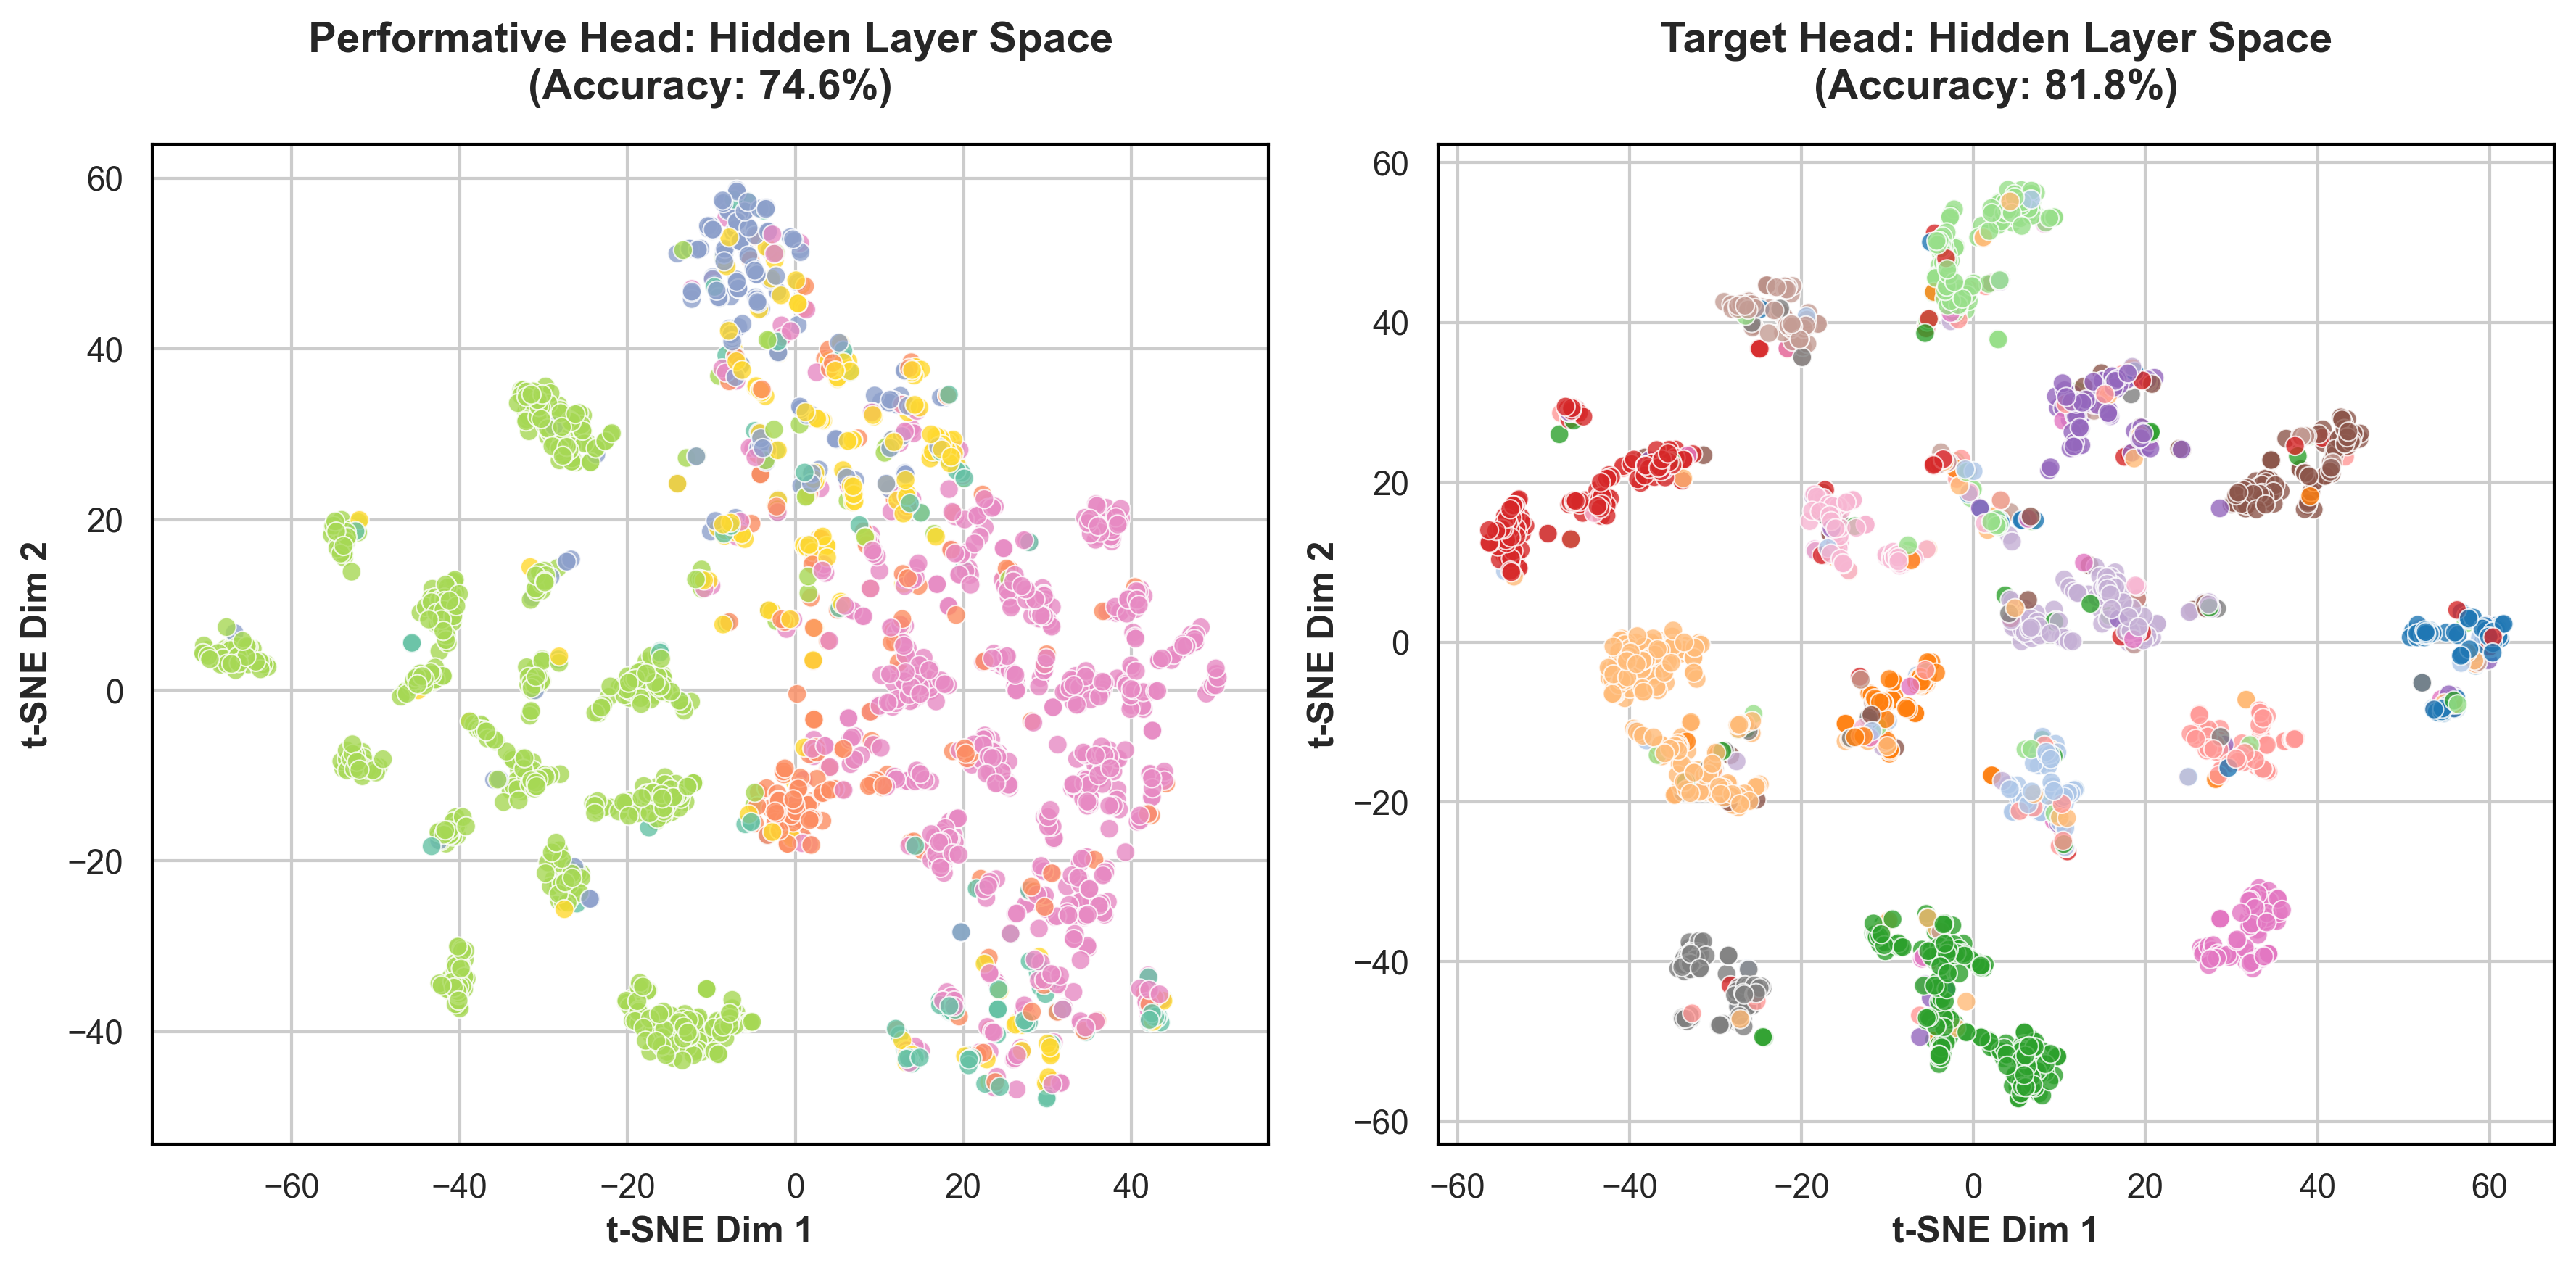
\includegraphics[width=1\textwidth]{images/NLP/finetuning/test_domain_adaptation.png}
    \caption{t-SNE projections of the hidden layers evaluated on the cross-model test set (\texttt{Qwen3.5:35b}). The disintegration of the previously distinct clusters visually explains the degradation in classification performance due to domain shift.}
    \label{fig:finetuning_domain_adaptation_tsne}
\end{figure}

While the model maintained high accuracy on the in-distribution test set, the cross-model evaluation revealed a critical vulnerability to domain shift. Figure \ref{fig:finetuning_domain_adaptation_tsne} illustrates the geometric impact of processing the \texttt{Qwen3.5:35b} dataset. Unlike the perfectly segregated manifold observed during validation (Figure \ref{fig:finetuning_tsne}), the cross-model latent space exhibits severe structural collapse and overlapping decision boundaries. This manifold degradation provides direct geometric proof for the drop in classification performance: the \texttt{SimpleJointBERT} architecture partially overfit the specific lexical and syntactic artifacts of \texttt{Gemma4:31b}, failing to robustly generalize the extraction of pragmatic intent from the phrasing of an unseen generator.


\subsection{Results Summary}

Table \ref{tab:results_summary} provides a comprehensive quantitative comparison of all evaluated methodologies. The progression demonstrates the structural inability of frozen representations to capture pragmatic semantics, contrasted with the high efficacy and deterministic target-lookup capability of the end-to-end fine-tuned custom architecture.

\begin{table}[H]
    \centering
    \resizebox{\textwidth}{!}{
        \begin{tabular}{llcc}
            \hline
            \textbf{Technique} & \textbf{Dataset} & \textbf{Performative Acc. (\%)} & \textbf{Target Acc. (\%)} \\
            \hline
            Naive Baseline & --- & 16.67 & 6.67 \\
            Anchor-Based Classification & Validation & 22.22 & 8.02 \\
            SVM (Gaussian RBF) & Validation & 91.60 & 60.90 \\
            \hline
            \multirow{4}{*}{\texttt{Custom Architecture}} & Training & 100.00 & 100.00 \\
             & Validation & 94.20 & 97.30 \\
             & Test (In-Distribution) & 96.90 & 98.40 \\
             & \textbf{Test (Cross-Model)} & \textbf{74.60} & \textbf{81.80} \\
            \hline
        \end{tabular}
    }
    \caption{Summary of classification accuracies across methodologies and datasets.}
    \label{tab:results_summary}
\end{table}

Lastly, to allows for a run-time use of the model during the games, a python-based microservice (defined in the directory \texttt{BERT\_API}) was implemented, which exposes the fine-tuned model through a REST API. This allows the Jason agents to query the service in real-time during gameplay, providing the raw message text and receiving the predicted performative and target labels for downstream decision-making processes.

\section{Gameplay Results}
\label{sec:results}

For the sake of completeness, this final section presents quantitative results from gameplay where agents are homogeneously driven by the symbolic engine, followed by results from the LLM-driven agents. The analysis is based on a dataset collected from 100 simulated games for each configuration (200 games in total). The data was processed and visualized using the custom Python scripts provided in the \texttt{GAME\_STATS} folder to generate the figures below.

\subsection{Symbolic Agents' Gameplay}
The baseline game setup consisted of 3 Wolves and 12 Villagers (an arbitrary ratio chosen to attempt equilibrium), utilizing the rules described in Section \ref{subsec:modifiedRules}. The agents' behavior was exclusively driven by the symbolic engine, without any LLM involvement.

\begin{figure}[H]
    \centering
    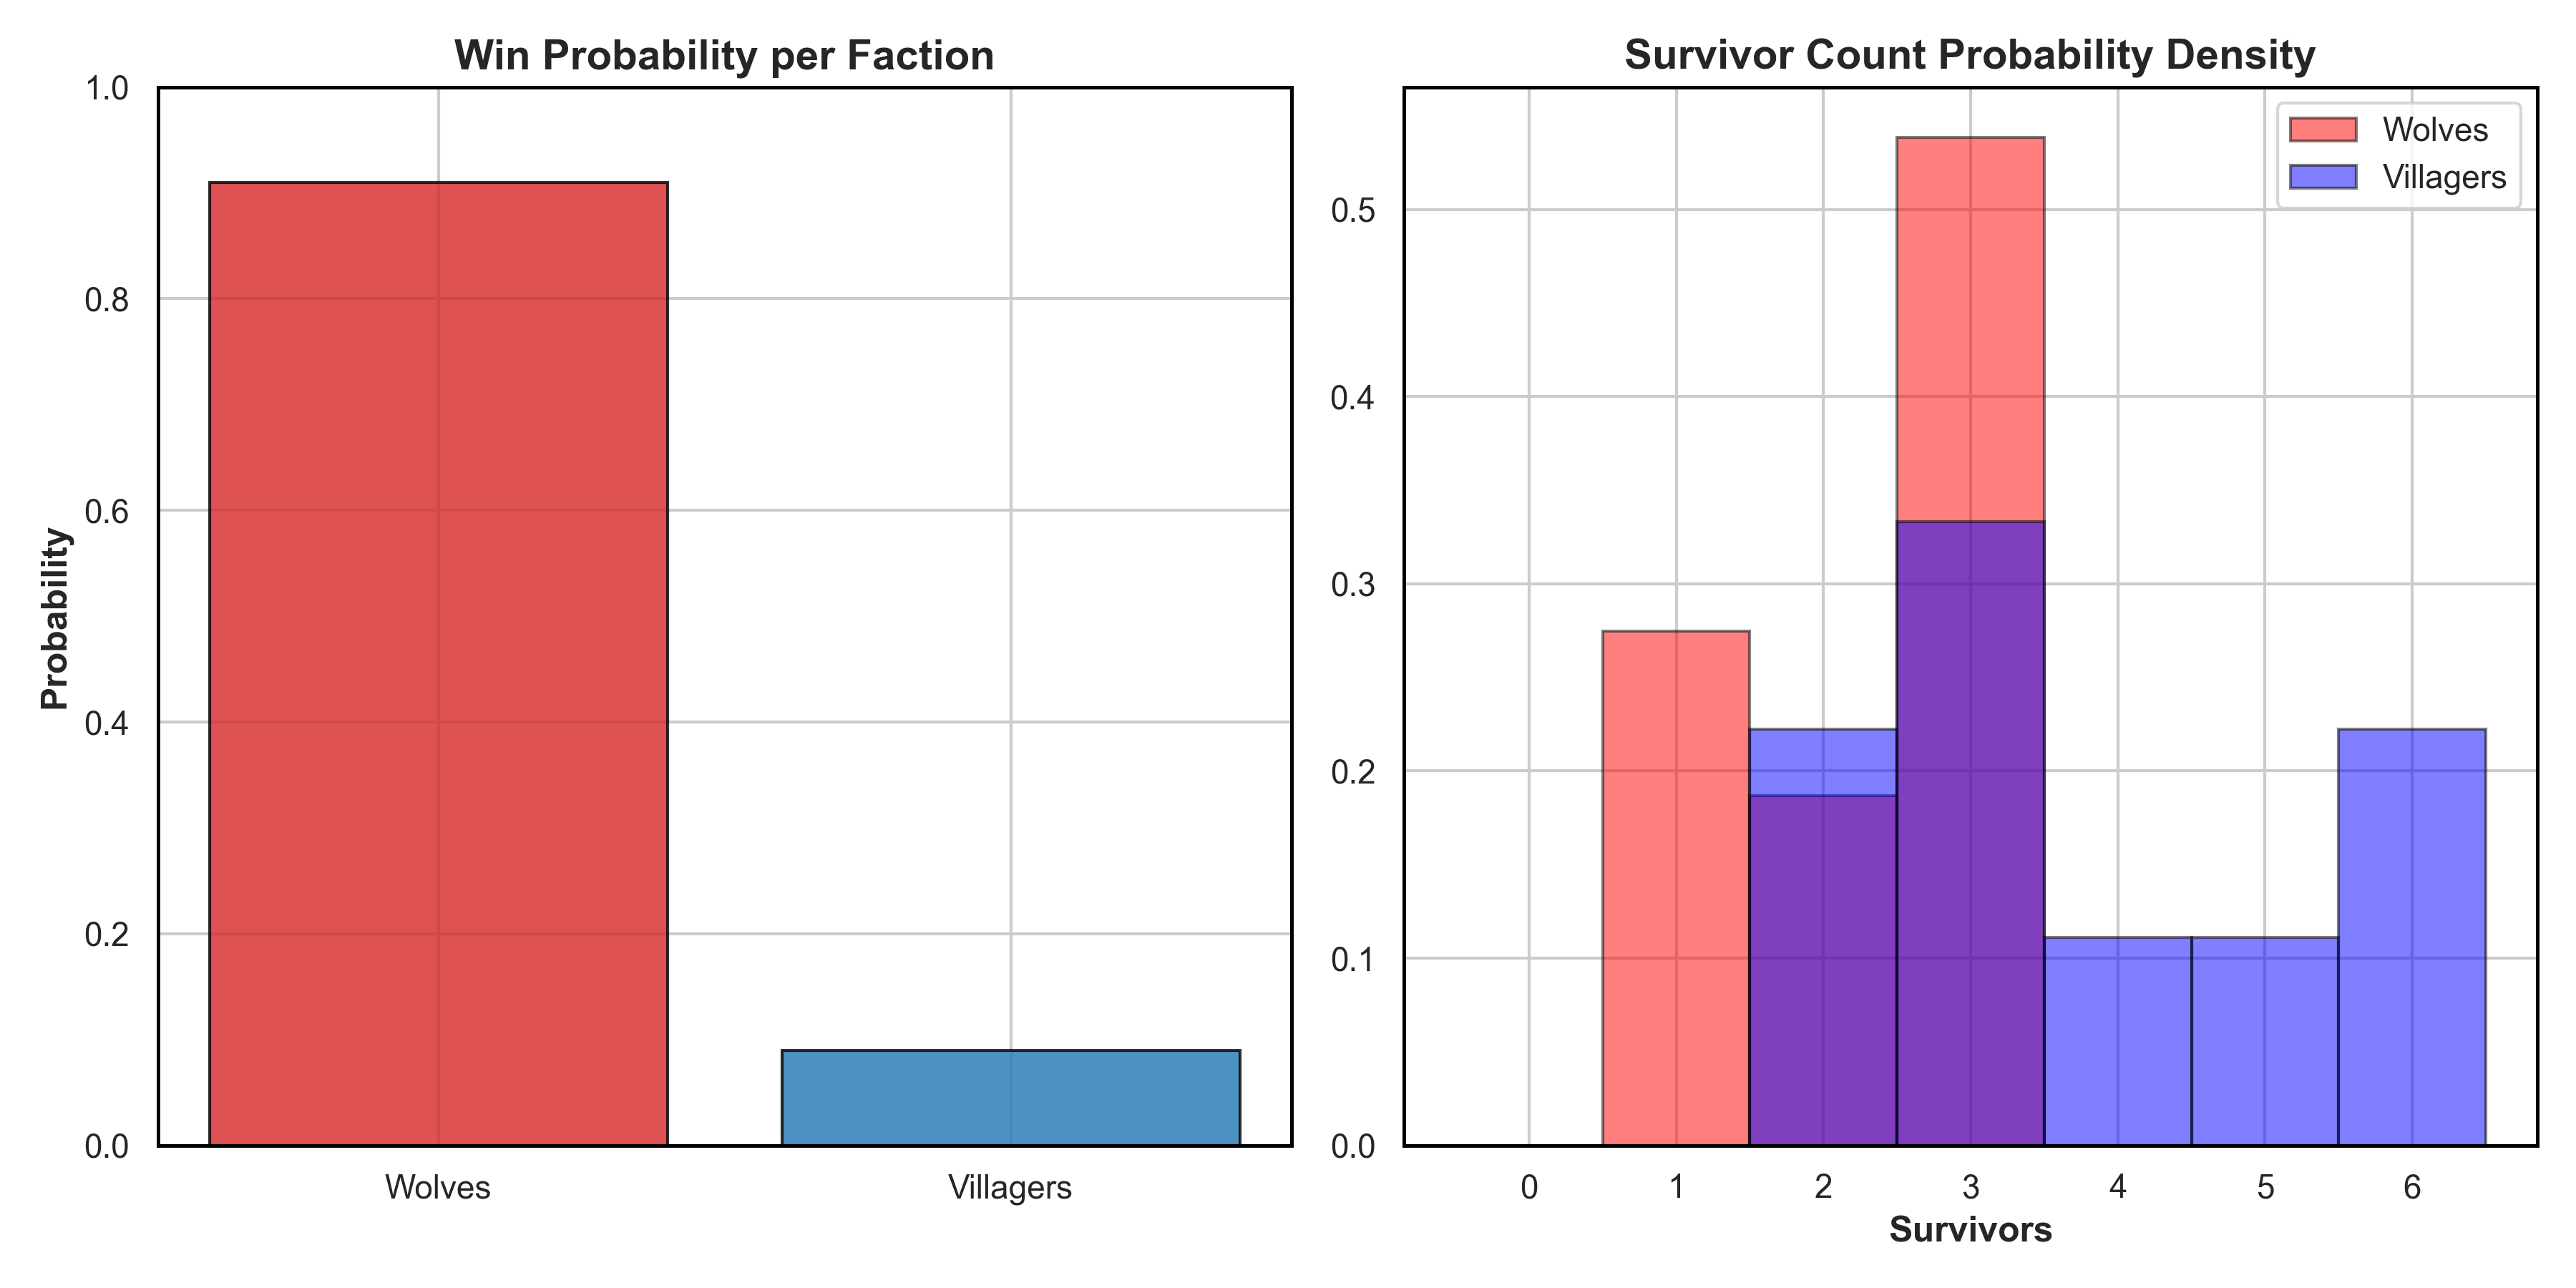
\includegraphics[width=1\textwidth]{images/game_results/symbolic_1.png}
    \caption{Win probability and survivor count density per faction.}
    \label{fig:symb_win_prob}
\end{figure}

Figure \ref{fig:symb_win_prob} demonstrates a severe structural imbalance in the pure symbolic setup. Despite a significant numerical disadvantage (3 vs. 12), the Wolf faction achieves a win rate exceeding 90\%. The survivor density further reflects this, showing that Wolves consistently maintain 1 to 3 survivors at the end of the game, whereas Villager victories are rare and yield higher survivor variance.

\begin{figure}[H]
    \centering
    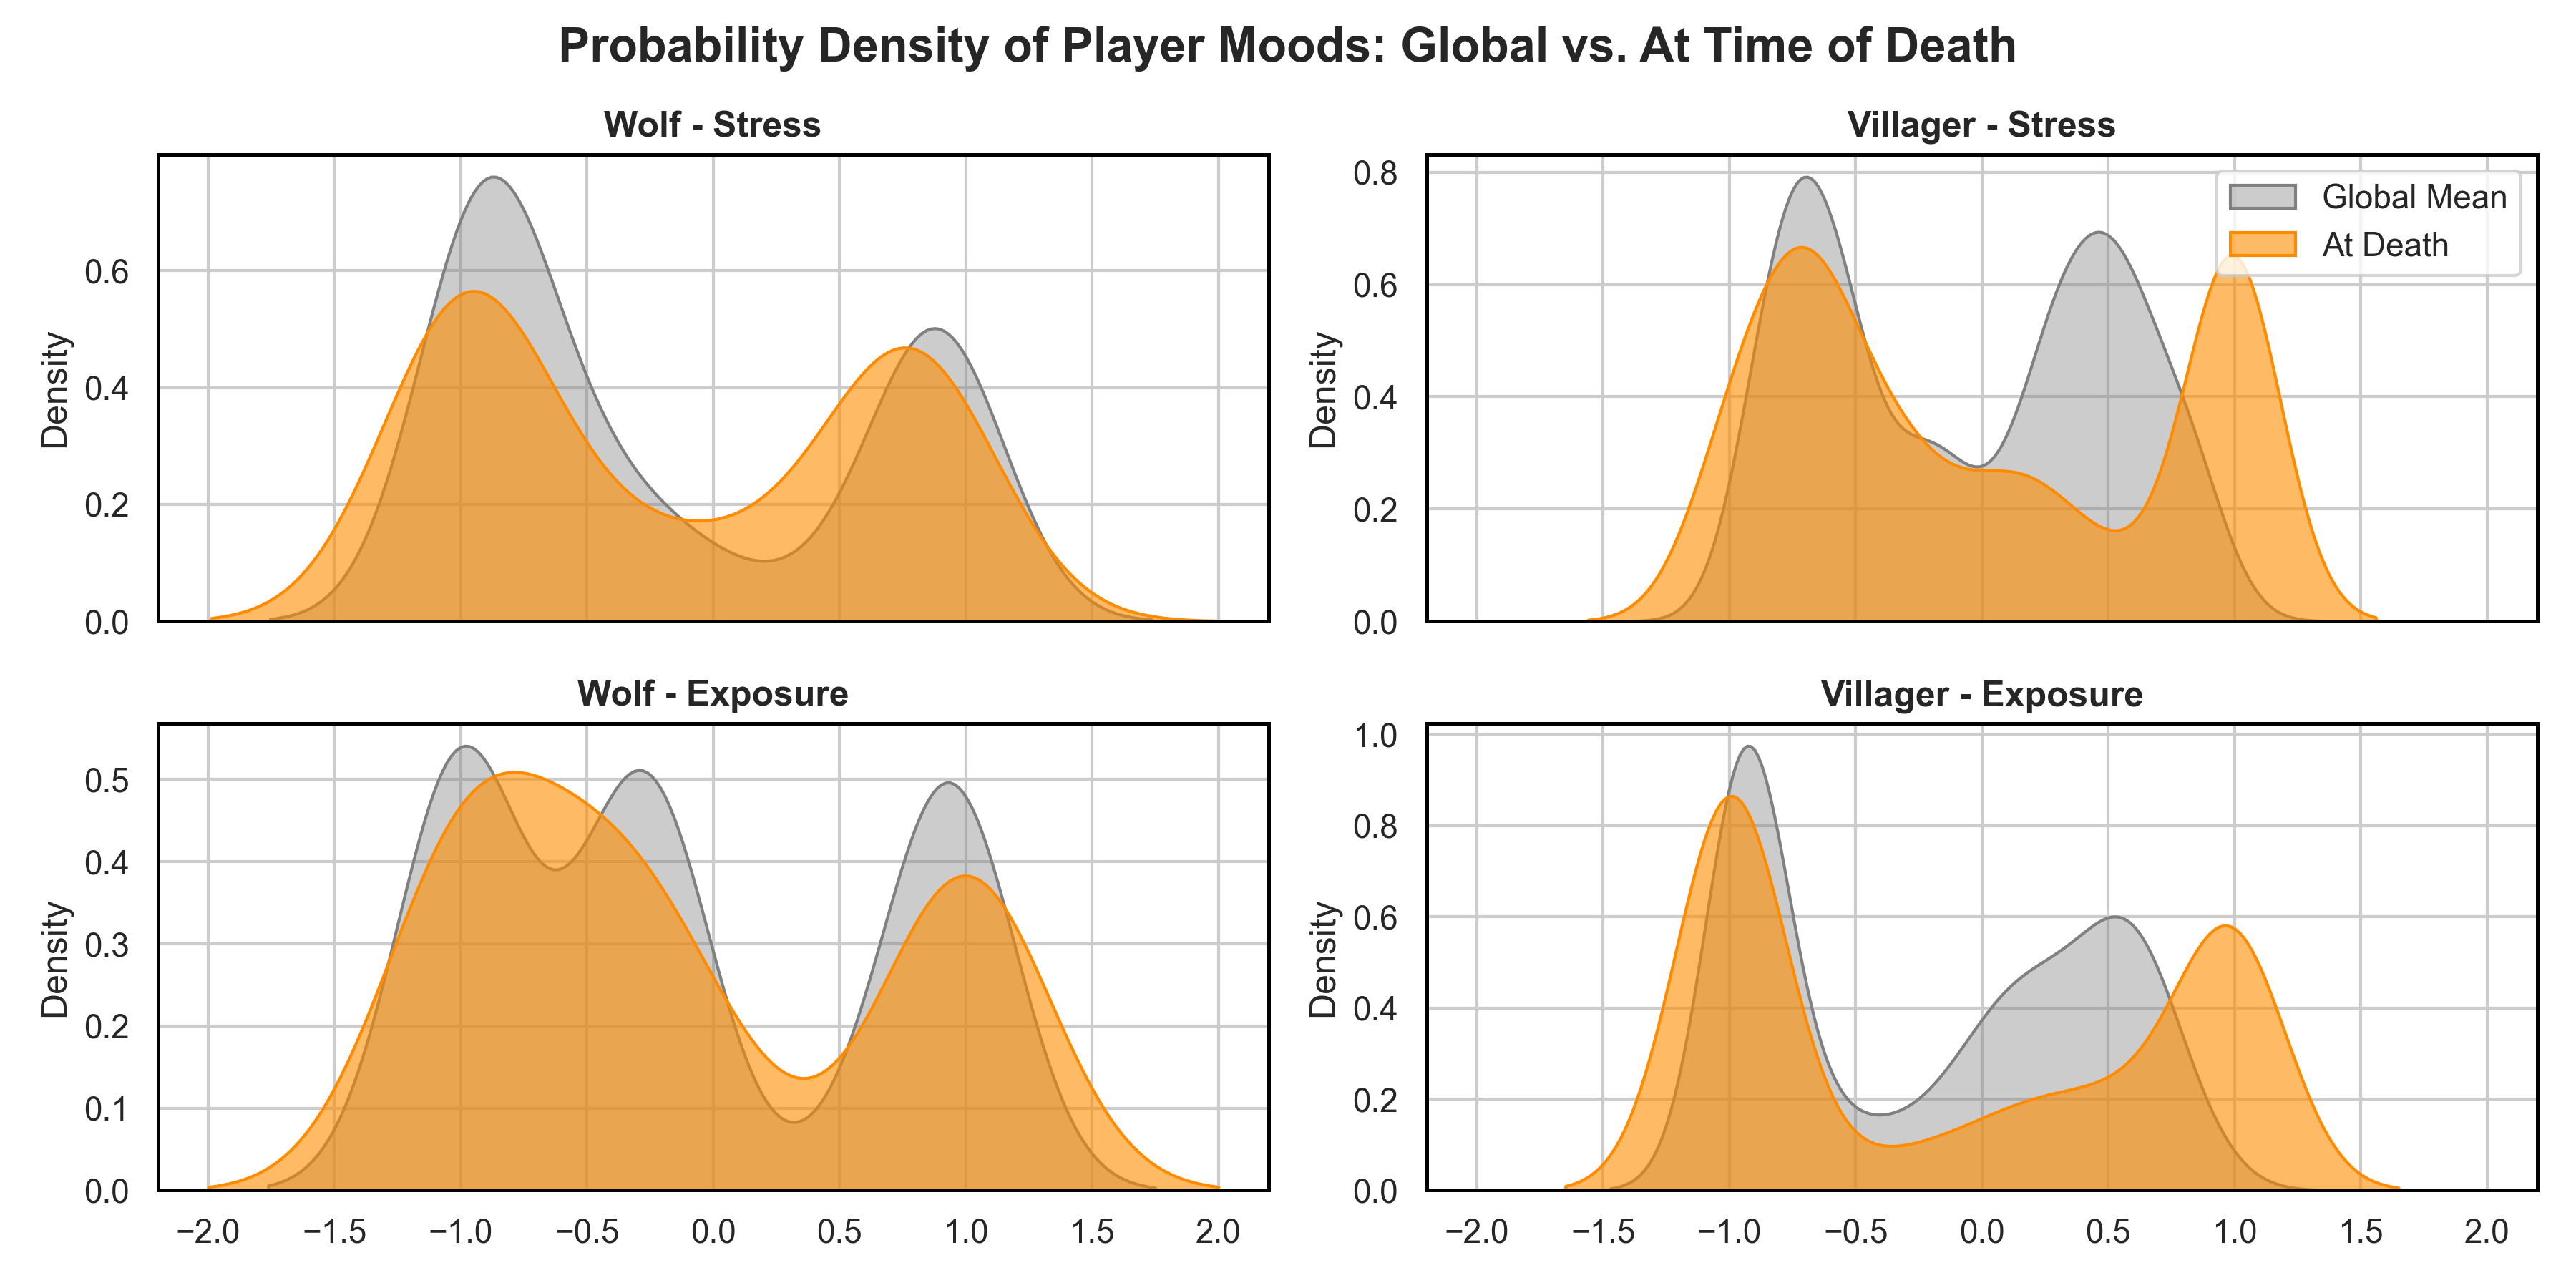
\includegraphics[width=1\textwidth]{images/game_results/symbolic_2.png}
    \caption{Density distributions of internal agent metrics (Stress and Exposure) comparing the global mean against the values recorded precisely at the time of the agent's death.}
    \label{fig:symb_metrics}
\end{figure}

Figure \ref{fig:symb_metrics} evaluates the internal state metrics of the agents. For both factions, but particularly for Villagers, the "At Death" density distribution (red) shows distinct right-side peaks compared to the "Global Mean" (blue). This indicates a strong positive correlation between elevated internal Stress/Exposure levels and in-game elimination, validating that the symbolic engine mathematically captures the danger state of the agents.

\begin{figure}[H]
    \centering
    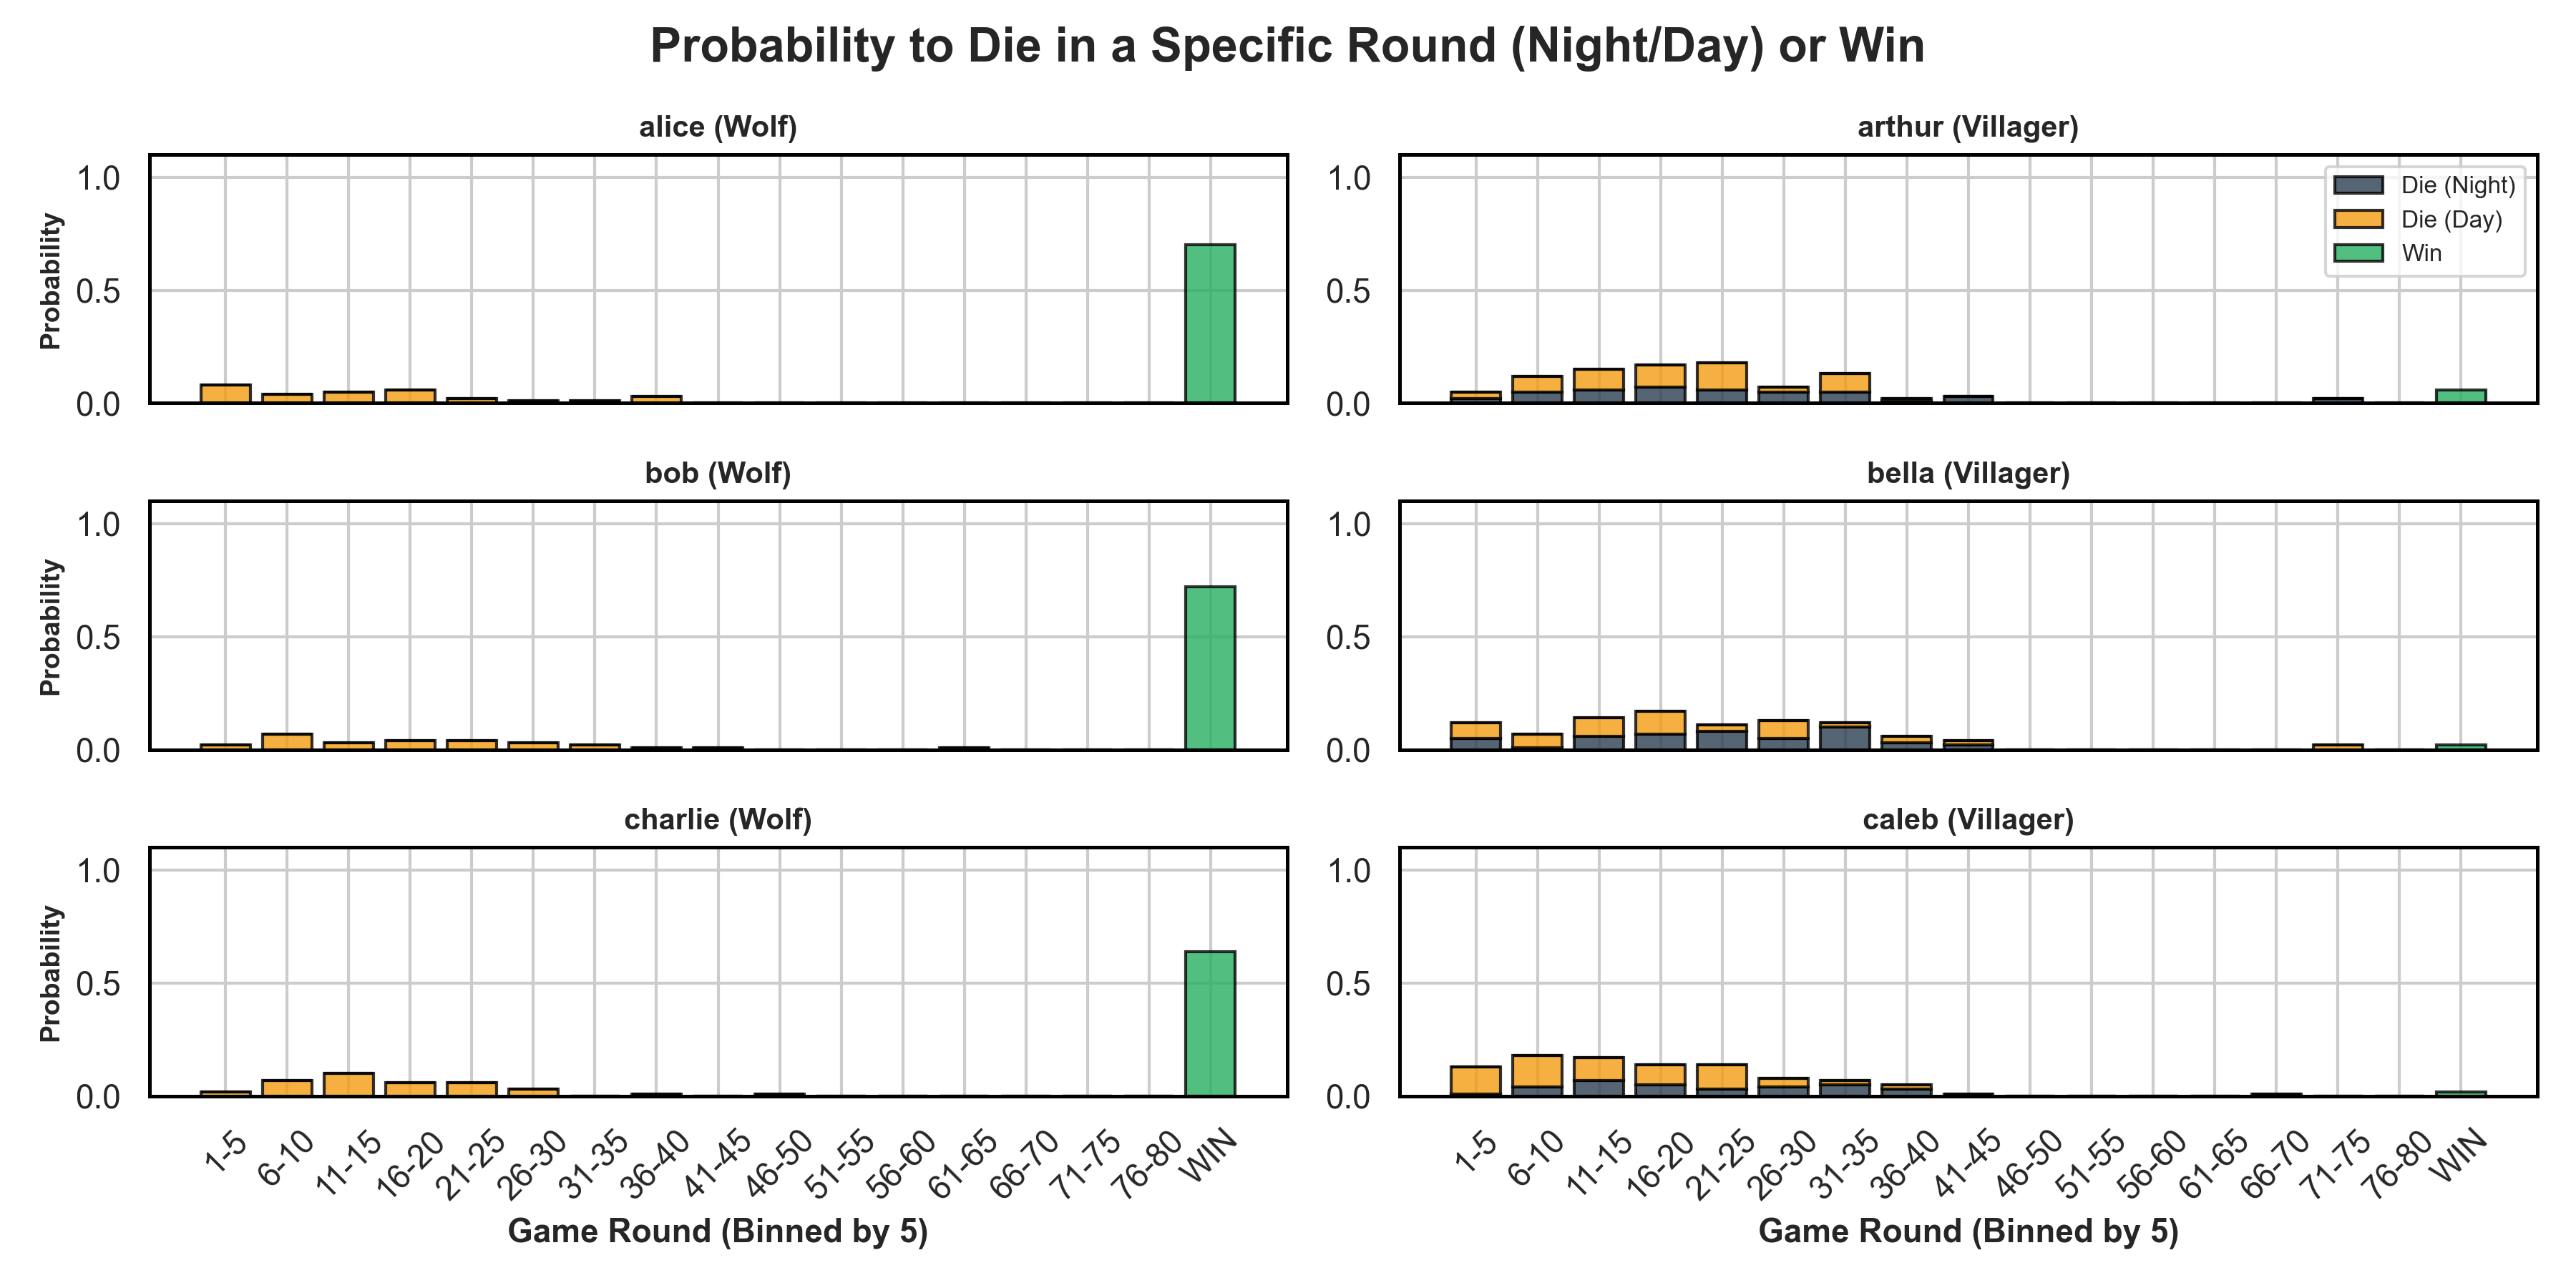
\includegraphics[width=1\textwidth]{images/game_results/symbolic_3.png}
    \caption{Probability distribution of player elimination across game rounds, segmented by Day/Night phases and ultimate Win state.}
    \label{fig:symb_survival}
\end{figure}

Finally, Figure \ref{fig:symb_survival} breaks down the temporal survival probabilities for specific agents. The data shows that Wolves (left column) experience minimal attrition, with very few deaths during the Day phase and zero at Night (confirming correct faction strategy implementation), overwhelmingly reaching the 'Win' state. Conversely, Villagers (right column) face steady, continuous elimination across the first 40 rounds, driven by a combination of Night (wolf attacks) and Day (incorrect lynching) phases.



\subsection{LLM-Driven Agents' Gameplay}


To test the LLM-driven agents (gemma4:31b), another set of simulations was conducted. Because processing natural language internal reasoning is computationally expensive, we scaled the game down to 12 players (3 Wolves and 9 Villagers). Even with this smaller roster, a single game took roughly 30 minutes using an externally hosted Ollama instance on an NVIDIA RTX 5090.

\begin{figure}[H]
    \centering
    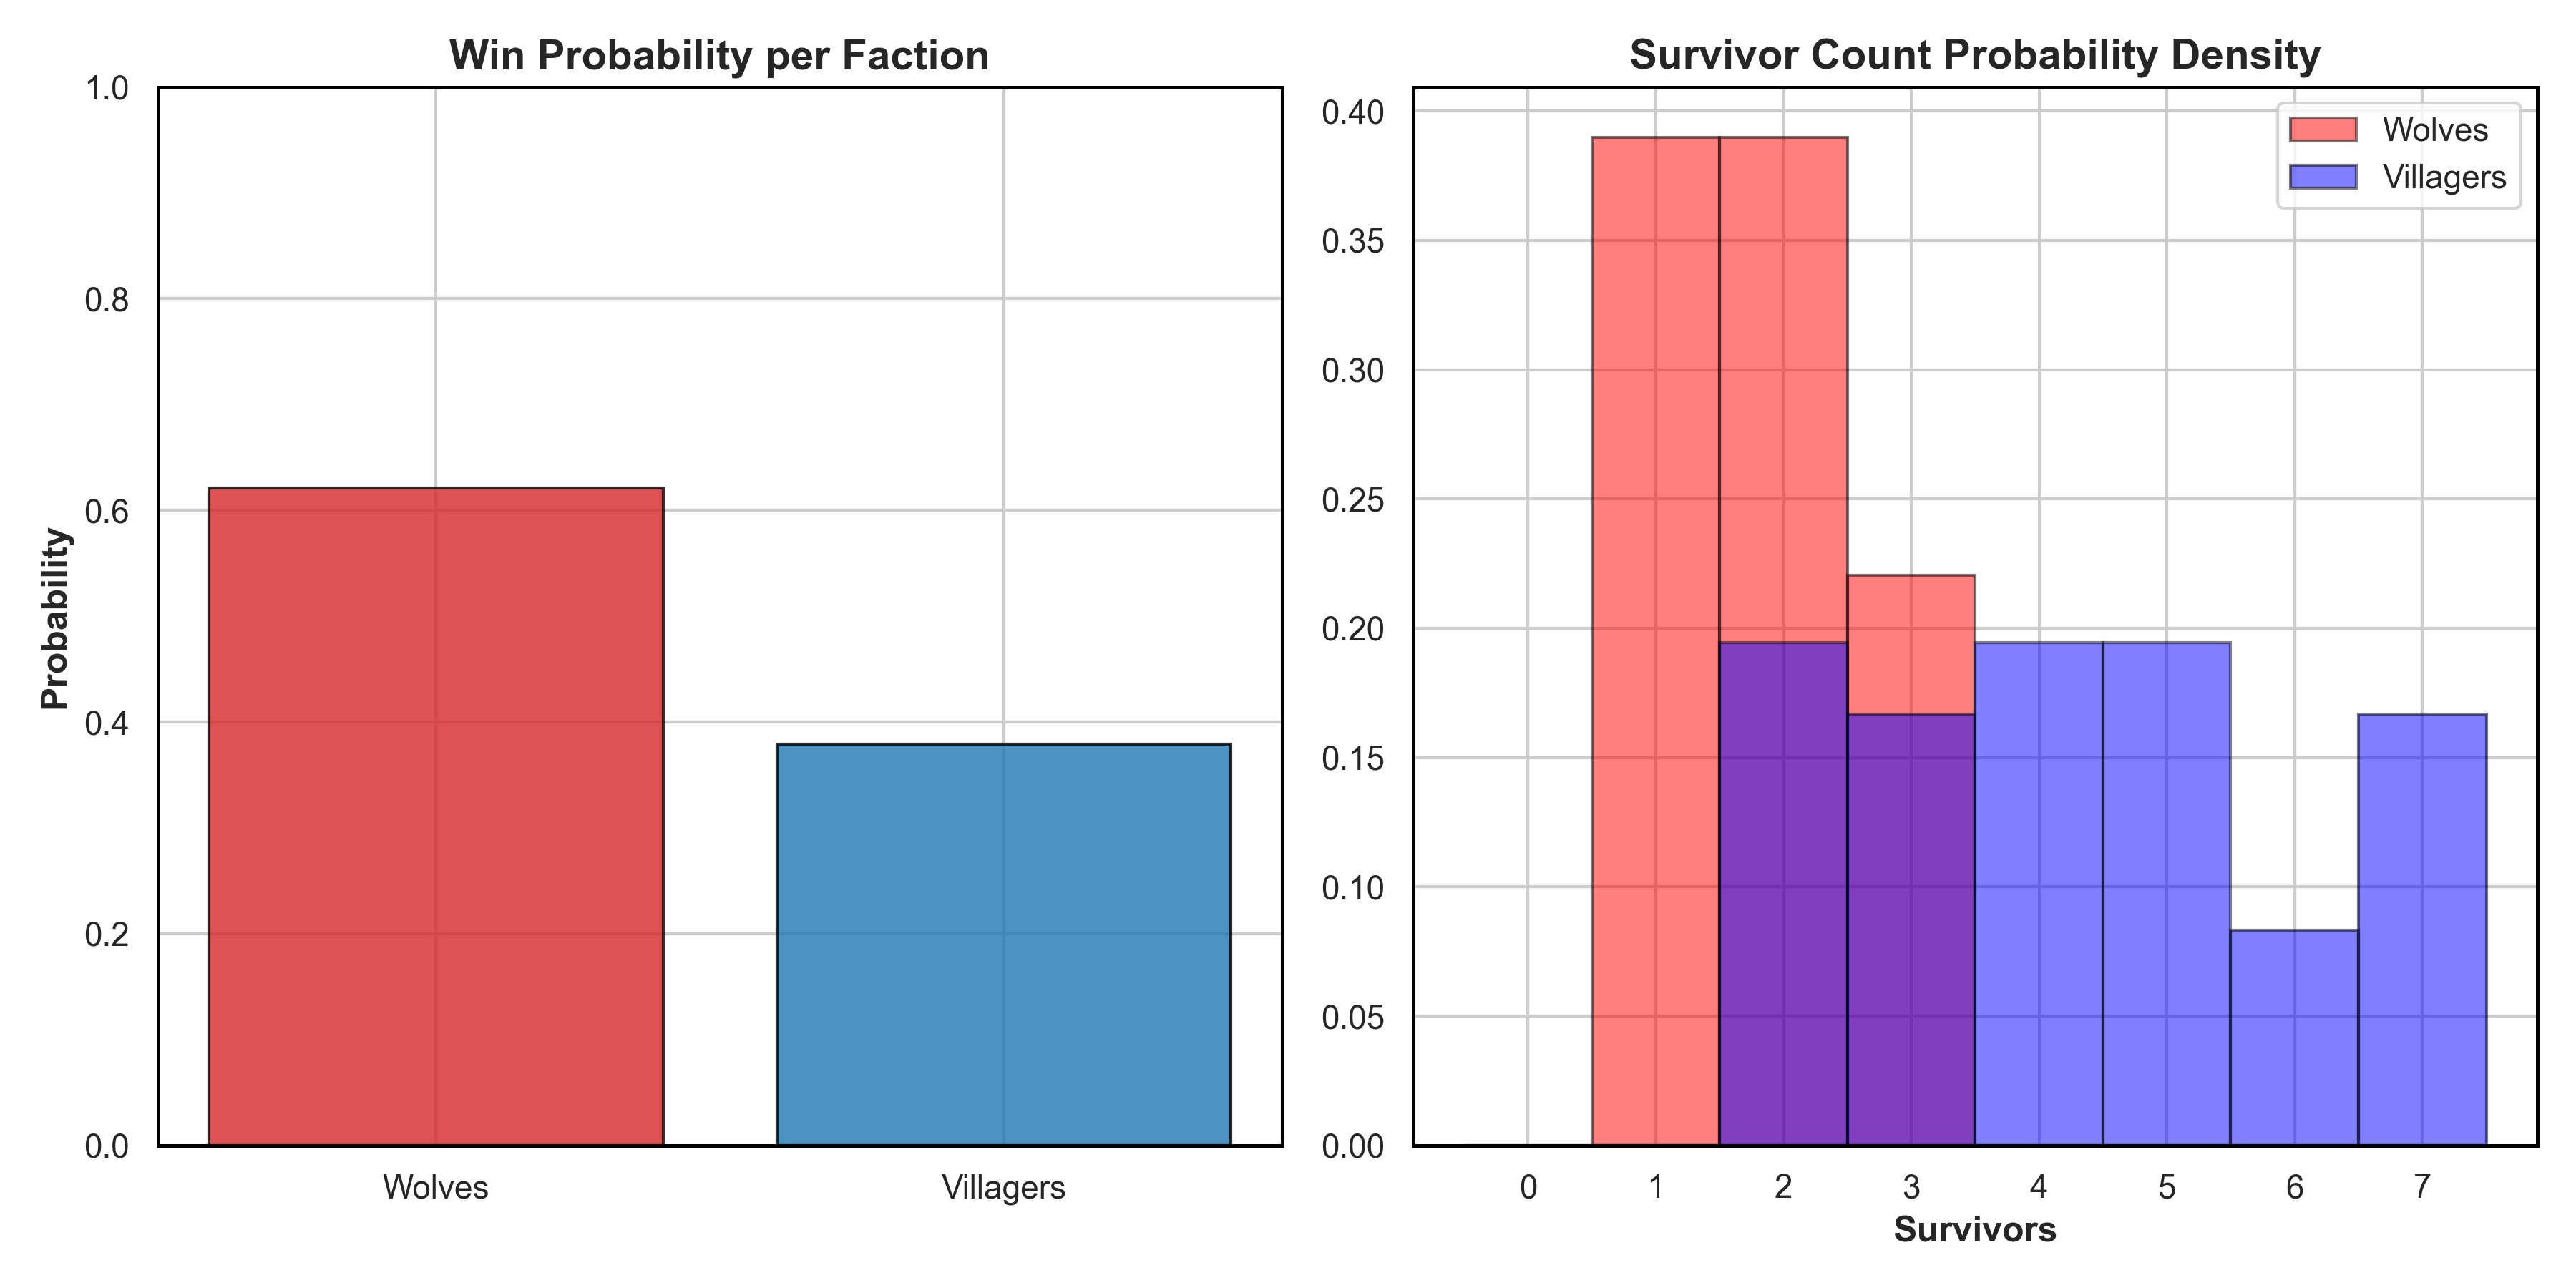
\includegraphics[width=1\textwidth]{images/game_results/llm_1.png}
    \caption{Win probability and survivor count density for LLM-driven agents.}
    \label{fig:llm_win_prob}
\end{figure}

Figure \ref{fig:llm_win_prob} shows that natural language reasoning drastically improves game balance. Compared to the purely symbolic baseline, the Wolf win rate drops from over 90\% to roughly 62\%, giving the Villagers a realistic 38\% chance to win.

\begin{figure}[H]
    \centering
    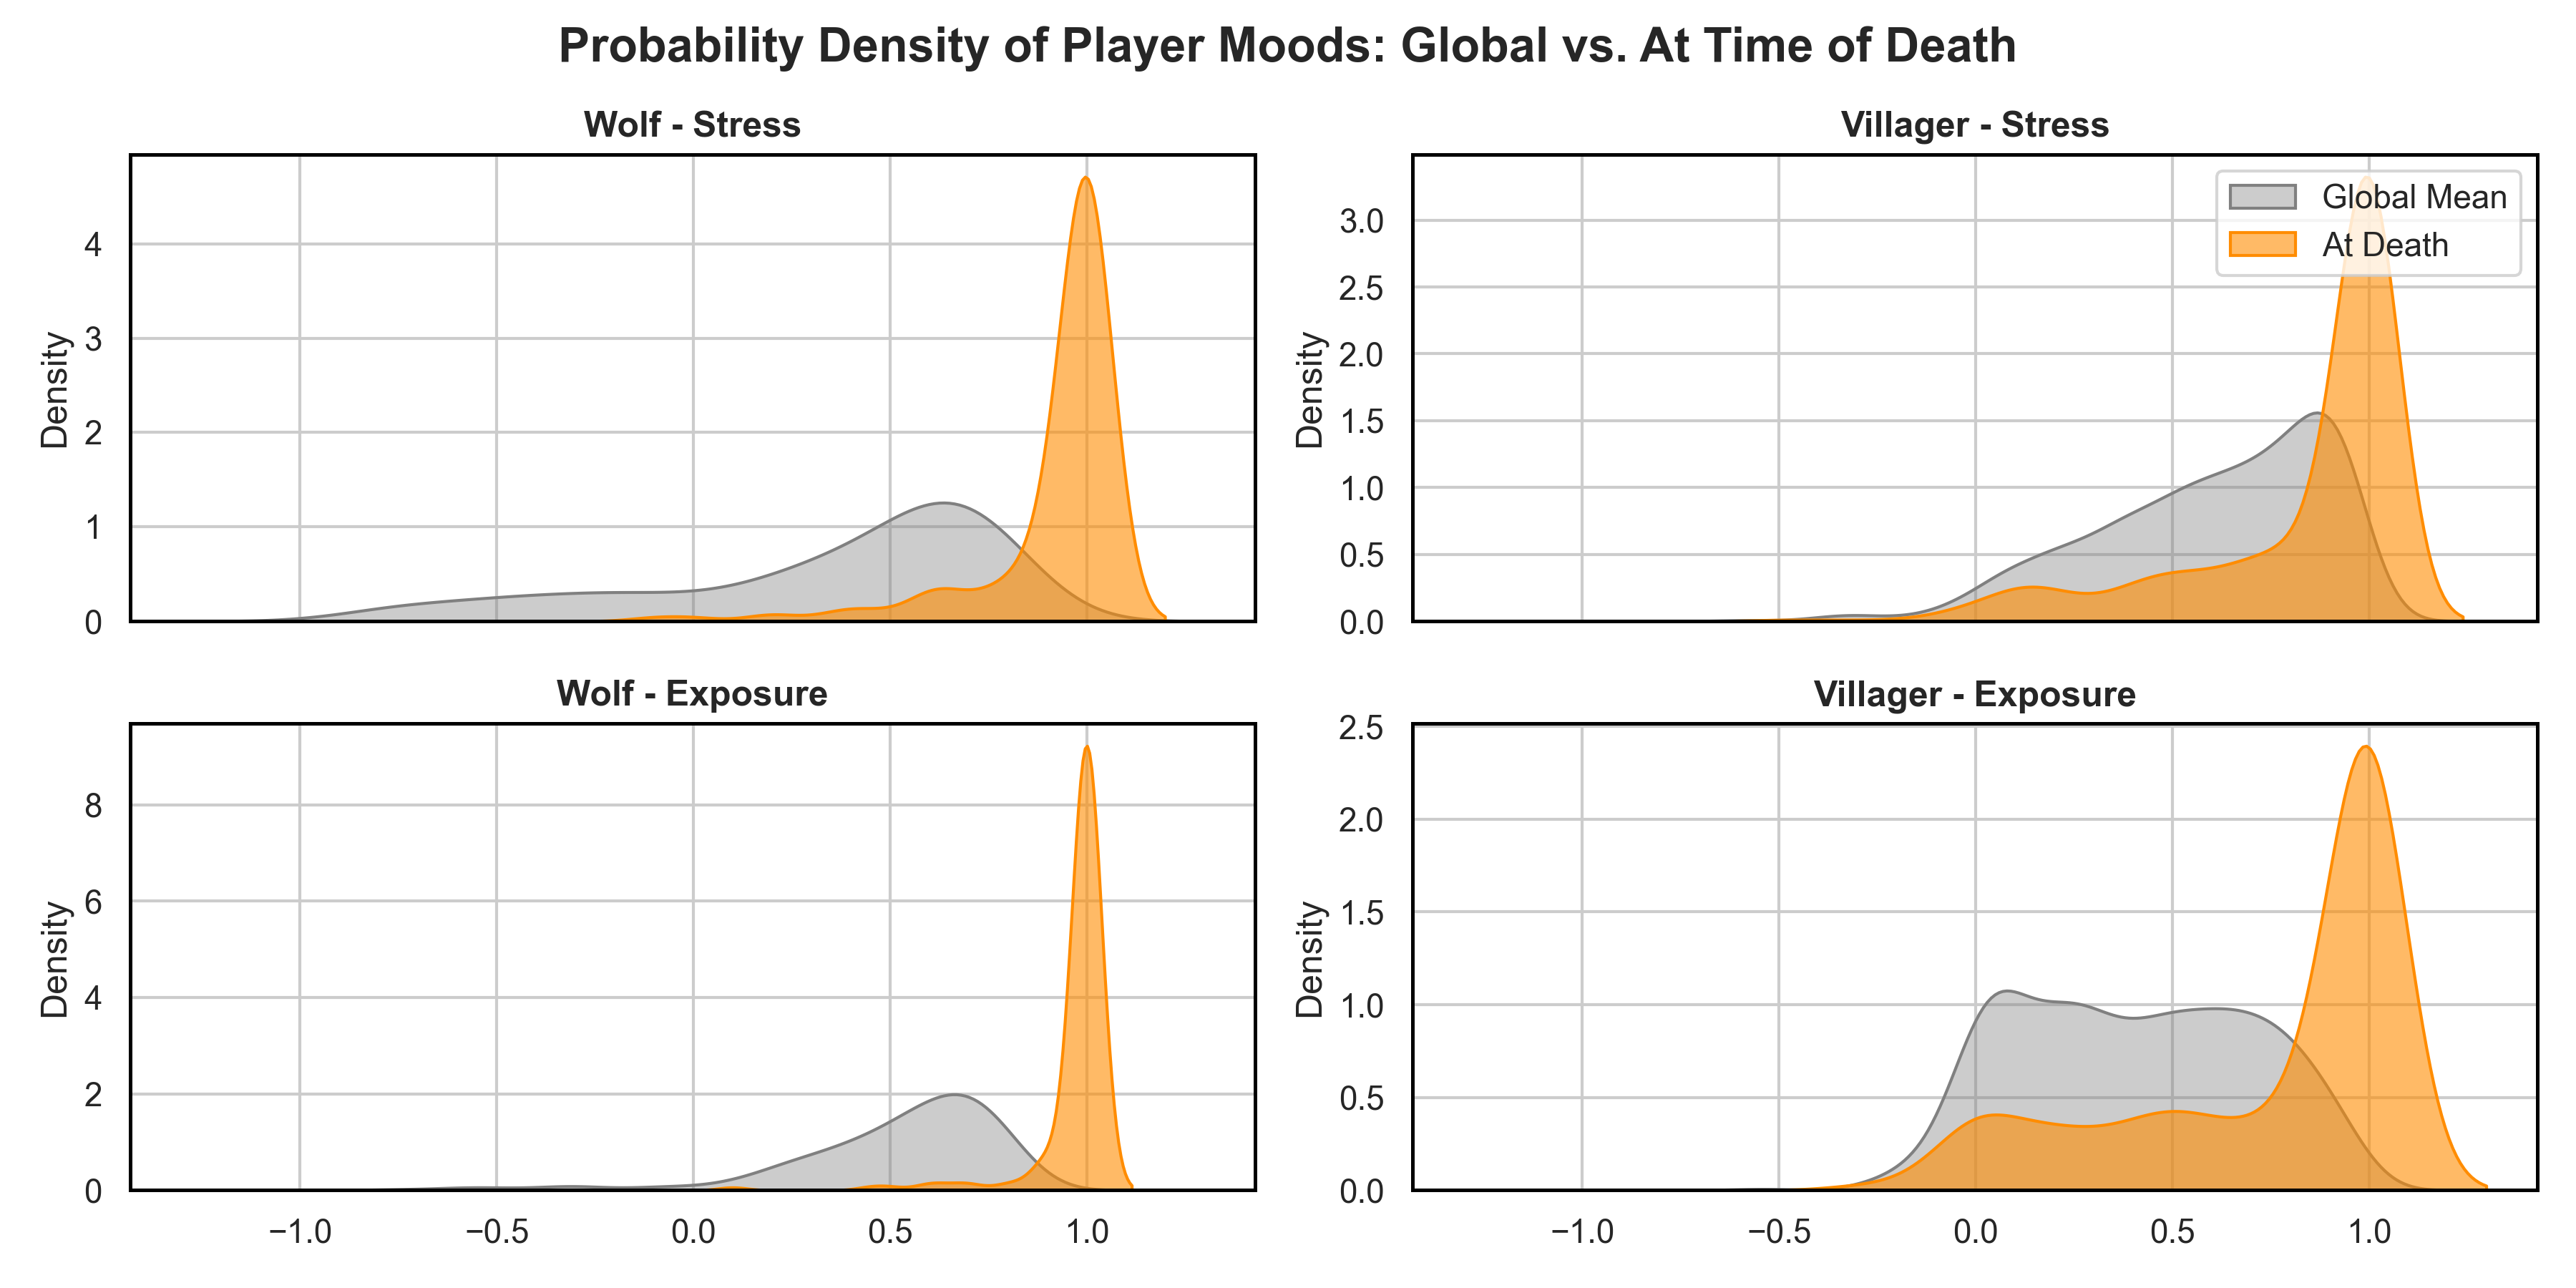
\includegraphics[width=1\textwidth]{images/game_results/llm_2.png}
    \caption{Density distributions of internal metrics (Stress and Exposure) for LLM-driven agents.}
    \label{fig:llm_metrics}
\end{figure}

Figure \ref{fig:llm_metrics} illustrates a major shift in how the agents handle internal metrics. Unlike the gradual curves of the symbolic engine, the LLM agents' stress and exposure spike sharply to 1.0 right before elimination. This proves the agents are highly aware of the game state: their metrics only max out when they correctly perceive they are in immediate, fatal danger.

\begin{figure}[H]
    \centering
    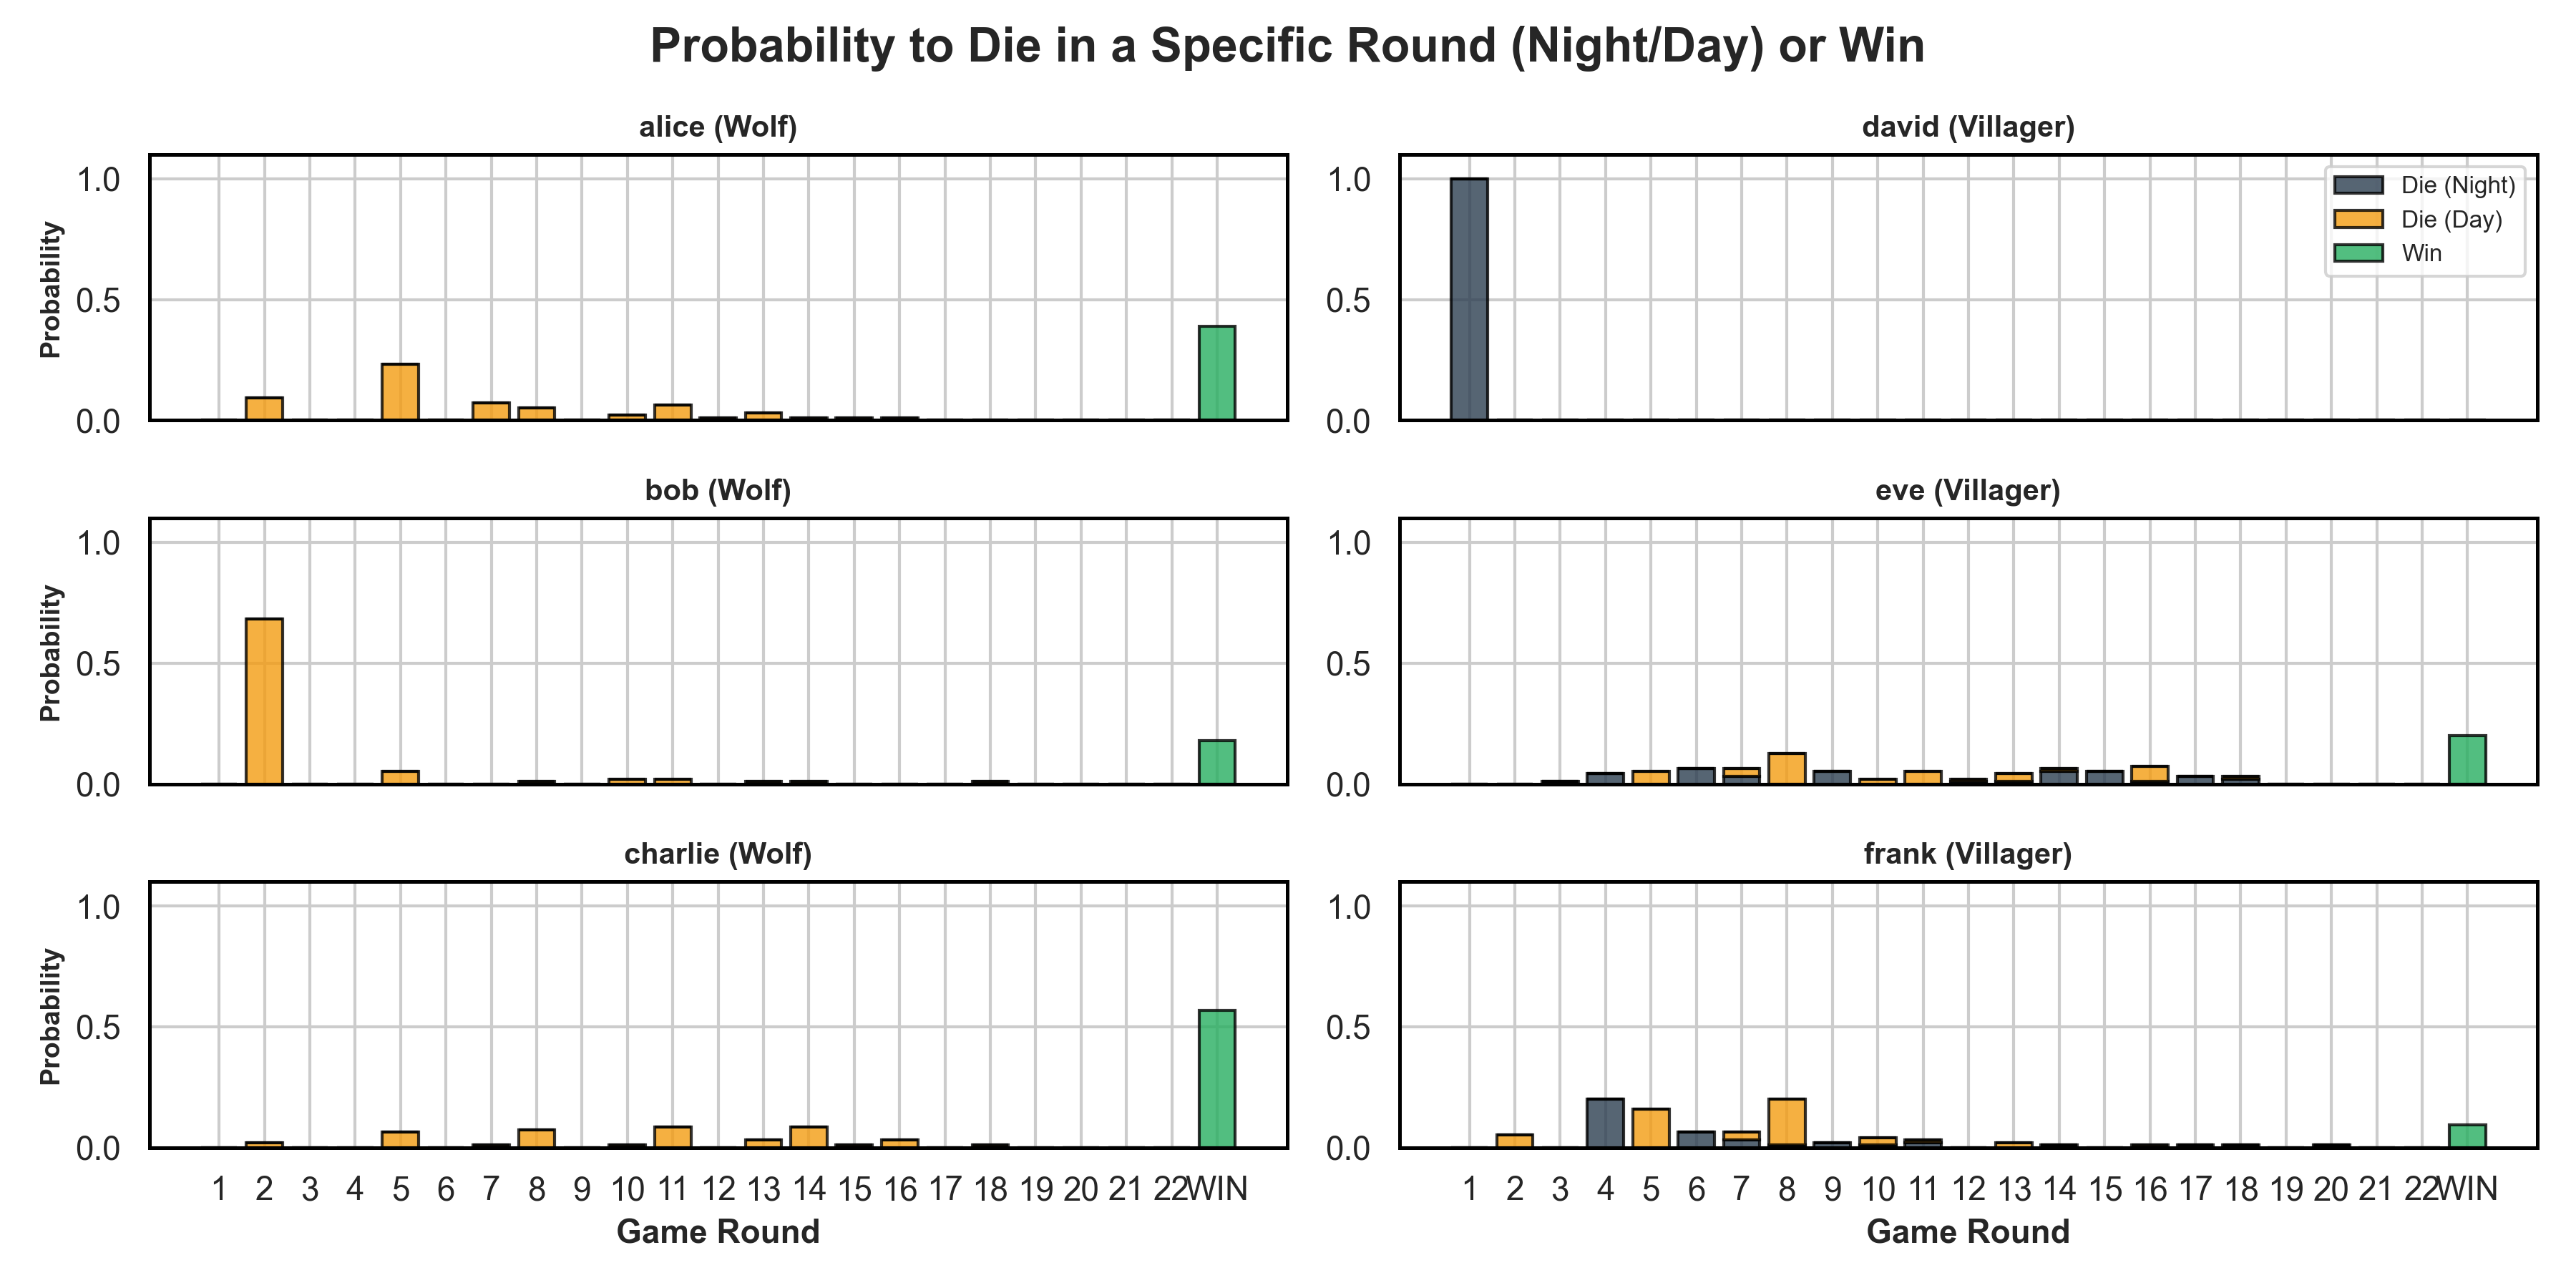
\includegraphics[width=1\textwidth]{images/game_results/llm_3.png}
    \caption{Probability distribution of player elimination across game rounds for LLM-driven agents.}
    \label{fig:llm_survival}
\end{figure}

Finally, Figure \ref{fig:llm_survival} highlights two distinct LLM behaviors. First, the games resolve much faster, typically ending within 20 rounds instead of 80. Second, the model shows severe targeting biases: the Villager 'david' is killed on Night 1 in almost every game, while the Wolf 'bob' is frequently lynched on Day 2. This suggests the underlying LLM relies on inherent lexical or contextual biases when selecting targets.

\paragraph{Emergent Biases in LLM Targeting}

The targeting behaviors observed in Figure \ref{fig:llm_survival} reveal a critical vulnerability in LLM-driven simulation: the manifestation of severe lexical biases. Despite strictly randomizing the order of player names in the prompt context and ensuring all agents started Round 1 with identical, "empty" internal states, the LLMs exhibited near-deterministic targeting. 

Specifically, the Villager 'david' was universally targeted by the Wolves on Night 1. Since the Wolf faction acts first and lacks any prior game context, this suggests the model defaulted to targeting the first alphabetically available Villager in its generated list.

More interestingly, the Wolf 'bob' was overwhelmingly targeted for lynching on Day 1. A hypothesized reason for this bypasses alphabetical sorting (which would target 'alice') and instead points to artifacts within the LLM's pre-training dataset. 

In computer science and cryptography literature, stereotypical transactional examples almost universally follow the format "Alice performs an action on Bob." Given that the system prompt explicitly commands the model to execute a target (\textit{"TASK: Cast your vote... Choose the player you want to eliminate"}), the LLM may inherently associate 'Bob' with the semantic role of the passive target or victim. These emergent behaviors demonstrate that without strict alignment safeguards, generative agents will substitute rational gameplay strategy with linguistic heuristics learned during pre-training.

\section{Conclusions and Future Work}
\label{sec:conclusions}

This project successfully demonstrated the viability of a hybrid Multi-Agent System (MAS) architecture for social deduction games. By seamlessly integrating the rigid, rule-based execution of Jason with the dynamic natural language generation and sub-symbolic reasoning of Large Language Models, the simulation achieved organic, highly interactive gameplay. Furthermore, the implementation of the custom fine-tuned BERT architecture effectively bridged the gap between ambiguous human-readable dialogue and strict logical performatives, allowing for a fully automated, closed-loop environment resilient to speech-act misalignment.

Despite these successes, the current architecture presents several structural limitations that pave the way for future developments:

\begin{itemize}
    \item \textbf{Higher-Order Epistemic Beliefs:} The current trait matrix is strictly limited to first-order beliefs. Implementing second-order beliefs like \textit{what Alice believes Bob thinks of her} would allow for significantly deeper Theory of Mind (ToM) modeling, enabling advanced manipulative strategies and complex deception.
    \item \textbf{Long-Term Strategic Planning:} By design, the current reasoning cycles are atomic and stateless. While this reduces computational overhead, it results in short-sighted players that can fall into behavioral loops. Future iterations must implement more sophisticated plan pools within the symbolic engine and introduce persistent intention stacks (or LLM "scratchpads"), allowing agents to formulate, track, and execute multi-phase strategies over several rounds.
    \item \textbf{Affective State Extraction from Text:} Currently, the NLP pipeline only extracts pragmatic intent and targets. A natural expansion would be inferring continuous internal states (such as a player's stress or exposure levels) directly from the raw text of their speeches. Initial experimentations utilizing Good Old-Fashioned AI (GOFAI) approaches, such as TF-IDF and Bag-of-Words, were discarded due to poor performance (yielding a Mean Absolute Error of $\approx 0.3$). Future solutions could better tackle this challenge.
\end{itemize}
\bibliographystyle{splncs04}
\bibliography{bibliography}

\end{document}